%=====================================================================
%  ANÁLISIS DEL ENTORNO Y DESARROLLO DE APLICACIONES MÓVILES
%  Informe técnico — Rediseño moderno
%  Compilable con pdfLaTeX (TeX Live 2022+)
%=====================================================================
\documentclass[11pt,a4paper]{article}

%---------------------------------------------------------------------
%  CODIFICACIÓN
%---------------------------------------------------------------------
\usepackage[T1]{fontenc}
\usepackage[utf8]{inputenc}
\usepackage[spanish,es-nodecimaldot,es-noindentfirst]{babel}

%---------------------------------------------------------------------
%  TIPOGRAFÍA MODERNA  (sans-serif + mono)
%  Si 'lato' no está instalado en local, descomenta la línea de lmodern
%---------------------------------------------------------------------
\usepackage{lmodern}   % <-- fallback si falla lato en local
\renewcommand{\familydefault}{\sfdefault}

\usepackage[varqu,varl]{inconsolata}
\usepackage{microtype}
\usepackage{parskip}
\setlength{\parskip}{0.65em}
\linespread{1.05}

%---------------------------------------------------------------------
%  GEOMETRÍA
%---------------------------------------------------------------------
\usepackage[a4paper,top=2.6cm,bottom=2.4cm,left=2.1cm,right=2.1cm,headheight=18pt]{geometry}

%---------------------------------------------------------------------
%  PALETA MODERNA
%---------------------------------------------------------------------
\usepackage[table]{xcolor}
\definecolor{ink}{HTML}{1A1F36}
\definecolor{primary}{HTML}{4F46E5}
\definecolor{primarydark}{HTML}{3730A3}
\definecolor{accent}{HTML}{F59E0B}
\definecolor{accent2}{HTML}{EC4899}
\definecolor{mint}{HTML}{10B981}
\definecolor{sky}{HTML}{0EA5E9}
\definecolor{soft}{HTML}{F3F4F6}
\definecolor{muted}{HTML}{6B7280}
\definecolor{mid}{HTML}{9CA3AF}

%---------------------------------------------------------------------
%  GRÁFICOS Y CAJAS
%---------------------------------------------------------------------
\usepackage{graphicx}
\usepackage{float}
\usepackage{tikz}
\usetikzlibrary{calc,positioning,shapes.geometric,backgrounds,patterns,shadows}
\usepackage[most]{tcolorbox}
\usepackage{fontawesome5}

%---------------------------------------------------------------------
%  TABLAS
%---------------------------------------------------------------------
\usepackage{array}
\usepackage{booktabs}
\usepackage{tabularx}
\usepackage{xltabular}
\usepackage{longtable}
\usepackage{makecell}
\renewcommand{\arraystretch}{1.32}
\setlength{\tabcolsep}{6pt}
\setlength{\arrayrulewidth}{0.3pt}
\arrayrulecolor{mid}

%---------------------------------------------------------------------
%  VARIOS
%---------------------------------------------------------------------
\usepackage{enumitem}
\usepackage{titlesec}
\usepackage{titletoc}
\usepackage{fancyhdr}
\usepackage{ragged2e}
\usepackage{csquotes}
\usepackage{amssymb}

%---------------------------------------------------------------------
%  HIPERENLACES (SIEMPRE AL FINAL)
%---------------------------------------------------------------------
\usepackage[hidelinks]{hyperref}

\hypersetup{
	colorlinks=true,
	linkcolor=primary,
	urlcolor=sky,
	citecolor=accent,
	pdftitle={Análisis del entorno y desarrollo de aplicaciones móviles},
	pdfauthor={Adrián Velasco Mañas},
	pdfsubject={Análisis del entorno de desarrollo de aplicaciones móviles},
	bookmarksnumbered=true,
	breaklinks=true
}

%---------------------------------------------------------------------
%  ESTILO DE SECCIONES
%---------------------------------------------------------------------
\titleformat{\section}
{\normalfont\sffamily\bfseries\LARGE\color{ink}}
{\colorbox{primary}{\textcolor{white}{\sffamily\bfseries\large\,\thesection\,}}\hspace{0.55em}}
{0pt}
{}
[\vspace{0.35em}{\color{primary}\rule{\linewidth}{2.5pt}}]

\titleformat{name=\section,numberless}
{\normalfont\sffamily\bfseries\LARGE\color{ink}}
{}
{0pt}
{}
[\vspace{0.35em}{\color{primary}\rule{\linewidth}{2.5pt}}]

\titleformat{\subsection}
{\normalfont\sffamily\bfseries\Large\color{primarydark}}
{\textcolor{accent}{\sffamily\bfseries\thesubsection}}
{0.55em}
{}
[\vspace{-0.35em}{\color{primary!35}\rule{\linewidth}{1pt}}]

\titleformat{\subsubsection}
{\normalfont\sffamily\bfseries\large\color{ink}}
{\textcolor{accent}{\sffamily\bfseries\thesubsubsection}}
{0.5em}
{}
[]

\titlespacing*{\section}{0pt}{2.4ex plus 1ex minus .2ex}{1.5ex plus .2ex}
\titlespacing*{\subsection}{0pt}{2ex plus 1ex minus .2ex}{1ex plus .2ex}
\titlespacing*{\subsubsection}{0pt}{1.6ex plus 1ex minus .2ex}{0.8ex plus .2ex}

%---------------------------------------------------------------------
%  ÍNDICE MODERNO
%---------------------------------------------------------------------
\contentsmargin{1.2em}
\titlecontents{section}
[0em]
{\vspace{0.35em}\sffamily\bfseries\color{ink}}
{\makebox[2.4em][l]{\colorbox{primary}{\color{white}\ \thecontentslabel\ }}}
{\hspace*{2.4em}}
{\hfill\color{primary}\contentspage}
[\vspace{0.1em}{\color{primary!25}\hrule height 0.4pt}]

\titlecontents{subsection}
[2.6em]
{\vspace{0.1em}\sffamily\small\color{muted}}
{\textcolor{accent}{\thecontentslabel}\hspace{0.5em}}
{}
{\hfill\color{muted}\contentspage}

%---------------------------------------------------------------------
%  ENCABEZADO / PIE MODERNOS
%---------------------------------------------------------------------
\pagestyle{fancy}
\fancyhf{}
\fancyhead[L]{\color{muted}\sffamily\footnotesize\faMobile*\ \ Análisis del entorno móvil}
\fancyhead[R]{\color{muted}\sffamily\footnotesize\nouppercase{\leftmark}}
\fancyfoot[C]{%
	\tikz[baseline]{\node[fill=primary,text=white,rounded corners=4pt,
		inner sep=4pt,font=\sffamily\bfseries\footnotesize,minimum width=8mm]{\thepage};}%
}
\renewcommand{\headrulewidth}{0pt}
\renewcommand{\footrulewidth}{0pt}

\fancypagestyle{plain}{
	\fancyhf{}
	\fancyfoot[C]{%
		\tikz[baseline]{\node[fill=primary,text=white,rounded corners=4pt,
			inner sep=4pt,font=\sffamily\bfseries\footnotesize,minimum width=8mm]{\thepage};}%
	}
	\renewcommand{\headrulewidth}{0pt}
}

%---------------------------------------------------------------------
%  CAJAS MODERNAS
%---------------------------------------------------------------------
\newtcolorbox{notabox}[1][]{
	enhanced jigsaw, breakable,
	colback=sky!5, colframe=sky,
	boxrule=0pt, leftrule=4pt, arc=6pt,
	left=12pt, right=12pt, top=10pt, bottom=10pt,
	fontupper=\small, #1
}

\newtcolorbox{warnbox}[1][]{
	enhanced jigsaw, breakable,
	colback=accent!8, colframe=accent,
	boxrule=0pt, leftrule=4pt, arc=6pt,
	left=12pt, right=12pt, top=10pt, bottom=10pt,
	fontupper=\small, #1
}

\newtcolorbox{ideabox}[1][]{
	enhanced jigsaw, breakable,
	colback=mint!8, colframe=mint,
	boxrule=0pt, leftrule=4pt, arc=6pt,
	left=12pt, right=12pt, top=10pt, bottom=10pt,
	fontupper=\small, #1
}

\newtcolorbox{capturabox}[1][]{
	enhanced jigsaw, breakable,
	colback=accent2!5, colframe=accent2,
	boxrule=0.5pt, arc=6pt,
	left=12pt, right=12pt, top=10pt, bottom=10pt,
	fontupper=\small, #1
}

\newtcolorbox{fuentesbox}[1][]{
	enhanced jigsaw, breakable,
	colback=soft, colframe=muted!50,
	boxrule=0pt, leftrule=3pt, arc=4pt,
	left=10pt, right=10pt, top=8pt, bottom=8pt,
	fontupper=\footnotesize, #1
}

%---------------------------------------------------------------------
%  COMANDOS RÁPIDOS
%---------------------------------------------------------------------
\newcommand{\code}[1]{\texttt{\color{primary}#1}}
\newcommand{\archivo}[1]{\texttt{\color{accent!85!black}#1}}
\newcommand{\flecha}{\,$\rightarrow$\,}
\newcommand{\campo}[1]{\textbf{\color{primary}#1}}

% Marca de figura pendiente
\newcommand{\figpend}[2]{%
	\begin{capturabox}
		\textbf{\color{accent2!70!black}\faCamera\ \ Figura #1 --- pendiente de capturar.}%
		\par\smallskip #2
	\end{capturabox}%
}

%---------------------------------------------------------------------
%  INICIO
%---------------------------------------------------------------------
\begin{document}
	
	%=====================================================================
	%  PORTADA
	%=====================================================================
	\begin{titlepage}
		\begin{tikzpicture}[remember picture, overlay]
			\fill[white] (current page.north west) rectangle (current page.south east);
			
			\fill[primary]
			(current page.north west)
			-- (current page.north east)
			-- ([yshift=-17.5cm]current page.north east)
			-- ([yshift=-15.5cm]current page.north west)
			-- cycle;
			
			\fill[primarydark, opacity=0.35]
			([yshift=-15.5cm]current page.north west)
			-- ([yshift=-17.5cm]current page.north east)
			-- ([yshift=-17.5cm]current page.north west)
			-- cycle;
			
			\fill[accent]  ([xshift=-2.6cm, yshift=-4.5cm]current page.north east) circle (2.6cm);
			\fill[accent2] ([xshift=-6.4cm, yshift=-8.2cm]current page.north east) circle (1.15cm);
			\fill[sky]     ([xshift=-0.9cm, yshift=-1.8cm]current page.north east) circle (0.55cm);
			\fill[mint]    ([xshift=-8.8cm, yshift=-2.2cm]current page.north east) circle (0.35cm);
			
			\node[white, opacity=0.06] at ([xshift=-4.5cm, yshift=-12.5cm]current page.north east)
			{\fontsize{230}{230}\selectfont\faMobile*};
			
			\foreach \x in {0,...,12} {%
				\foreach \y in {0,...,9} {%
					\pgfmathsetmacro{\dotx}{1.4+\x*0.55}%
					\pgfmathsetmacro{\doty}{-9.5-\y*0.55}%
					\fill[white, opacity=0.18]
					([xshift=\dotx cm, yshift=\doty cm]current page.north west)
					circle (0.024cm);
				}%
			}
			
			\fill[accent] (current page.south west) rectangle ([yshift=0.55cm]current page.south east);
		\end{tikzpicture}
		
		\vspace*{1.3cm}
		\begin{flushleft}
			\hspace*{1.6cm}%
			{\color{accent}\sffamily\bfseries\footnotesize\faMobile*\ \ MÓDULO PROFESIONAL}\\[0.35em]
			\hspace*{1.6cm}%
			{\color{white}\sffamily\small Desarrollo de Aplicaciones Móviles}
		\end{flushleft}
		
		\vspace{2.8cm}
		\begin{flushleft}
			\hspace*{1.6cm}%
			{\color{white}\sffamily\fontsize{40}{44}\selectfont\bfseries Análisis del entorno}\\[0.1em]
			\hspace*{1.6cm}%
			{\color{white}\sffamily\fontsize{40}{44}\selectfont\bfseries y desarrollo de}\\[0.1em]
			\hspace*{1.6cm}%
			{\color{accent}\sffamily\fontsize{40}{44}\selectfont\bfseries aplicaciones móviles}
		\end{flushleft}
		
		\vspace{1.1cm}
		\begin{flushleft}
			\hspace*{1.6cm}%
			{\color{white!75!primary}\sffamily\large Investigación, análisis y configuración de un entorno de desarrollo.}
		\end{flushleft}
		
		\vfill
		\begin{flushleft}
			\hspace*{1.6cm}%
			\begin{tcolorbox}[enhanced,
				width=15cm,
				colback=white, colframe=primary!15,
				boxrule=1pt, arc=10pt,
				drop shadow={opacity=0.10, shadow xshift=3pt, shadow yshift=-3pt},
				left=16pt, right=16pt, top=14pt, bottom=14pt]
				\begin{tabular}{@{}>{\sffamily\bfseries\color{primary}}p{3cm} >{\sffamily\color{ink}}p{10cm}@{}}
					Nombre      & \textit{Adrián Velasco Mañas} \\[0.35em]
					Curso       & \textit{2º DAMP (Desarrollo de Aplicaciones Multiplataforma)} \\[0.35em]
					Módulo      & \textit{Programación multimedia y dispositivos móviles} \\[0.35em]
					Entrega     & \textit{04/10/2026} \\
				\end{tabular}
			\end{tcolorbox}
		\end{flushleft}
		
		\vspace{1cm}
	\end{titlepage}
	
	%=====================================================================
	%  ÍNDICE
	%=====================================================================
	\newpage
	{\sffamily
		\renewcommand{\contentsname}{\color{ink}\sffamily\bfseries\Huge Índice}
		\tableofcontents
	}
	\thispagestyle{plain}
	
	%=====================================================================
	%  APARTADO 1
	%=====================================================================
	\section{Análisis de las limitaciones de los dispositivos móviles}
	
	\subsection{Identificación de las principales limitaciones}
	
	Un dispositivo móvil es un ordenador con unas restricciones que no aparecen en un portátil de sobremesa: los recursos no son infinitos, la energía se agota y el usuario se lo lleva a todas partes (y eso incluye ascensores, trenes y zonas sin cobertura). Las limitaciones que explico a continuación son las que más veces se repiten cuando hay un problema real.
	
	\subsubsection*{1 - Memoria RAM limitada}
	
	\campo{¿En qué consiste?}
	Sabemos que la memoria RAM se utiliza para guardar datos temporales y procesos que se usan en el móvil, además de usarse para que el sistema operativo y las aplicaciones puedan funcionar correctamente, así que al desarrollar una aplicación móvil hay que saber gestionar la memoria para que el equipo pueda funcionar bien.
	
	\campo{¿Por qué afecta a una aplicación?}
	Una aplicación que use demasiada memoria puede hacer que el sistema se vea obligado a cerrar otras aplicaciones que estaban en segundo plano (o forzar el cierre de la aplicación).
	
	\campo{Ejemplo práctico.}
	Imaginemos una aplicación de edición de imágenes que carga archivos de alta resolución en la memoria. Si se utiliza en un dispositivo con poca RAM, la aplicación puede lentizar el sistema o incluso puede cerrarse porque el sistema se vea obligado a hacerlo.
	
	\campo{¿Cómo se soluciona?}
	La solución más evidente es optimizar el consumo de memoria pero, ¿cómo se hace? Normalmente, liberar objetos del código o recursos que no se utilizan pueden reducir el consumo, aunque hay más cosas que podemos hacer, como no cargar todas las imágenes al mismo tiempo (tendríamos que cargarlas poco a poco), además de reducir la resolución de estas. También podemos usar una técnica llamada \href{https://es.wikipedia.org/wiki/Lazy_loading}{lazy loading}, que retrasa la carga de un recurso o fragmento de código hasta el momento en que se necesita.
	
	Lo que no es tan obvio es que el límite \emph{no es el mismo en todos los móviles}. Android va publicando en su documentación unas tablas de \enquote{comportamiento incorrecto} (\emph{bad behavior}) que dependen de la gama de RAM del dispositivo: para una app en primer plano el límite va desde 2,00 GB en un móvil de 4 GB hasta 4,25 GB en uno de 16 GB o más. O sea, el mismo código consume el doble de margen en un gama alta que en uno de gama baja, y el sistema lo cierra antes de que te enteres.
	
	\subsubsection*{2 - Potencia de procesamiento limitada}
	
	\campo{¿En qué consiste?}
	No todos los teléfonos tienen la misma capacidad de procesamiento ni todos gestionan de la misma manera los procesos asociados al rendimiento, al consumo ni a la temperatura. Un dispositivo con poca potencia de procesamiento puede tener dificultades para ejecutar operaciones dentro de nuestras aplicaciones, dificultades que en un dispositivo de alta gama no tendría.
	
	\campo{¿Por qué afecta a una aplicación?}
	Si dentro de nuestra aplicación se realizan demasiados cálculos, el dispositivo puede gastar muchos recursos del procesador para poder realizar estos cálculos, lo que provocaría lentitud en el móvil, poca fluidez (porque el procesador no podría ocuparse de todo al mismo tiempo y se emplearían menos recursos de lo normal en la interfaz gráfica), mucho tiempo de espera en operaciones (como abrir otras aplicaciones) y un mayor consumo de la batería (estresamos el procesador y este necesita alimentarse).
	
	Android pone dos APIs oficiales para preguntar al sistema con qué elementos o componentes estamos jugando:
	\code{ActivityManager.getMemoryClass()} devuelve en megabytes la memoria disponible para tu aplicación y \code{ActivityManager.isLowRamDevice()} te dice directamente si estás en un dispositivo de gama baja. Con eso ya no hay que adivinar nada, que no está nada mal para conocer en que dispositivos usan tu aplicaicón.
	
	\campo{Ejemplo práctico.}
	Imaginemos que desarrollamos un juego 3D (con los renderizados y shaders de C++ y sus librerías) e intentamos renderizar la parte gráfica de forma constante: si tenemos un dispositivo potente no habrá problema, pero con un móvil de gama baja el juego podría presentar una bajada de FPS y podría reducirse la fluidez de forma considerable.
	
	\campo{¿Cómo lo solucionamos?}
	Entre otras muchas cosas (como monitorear el rendimiento en partes del mapa con alto renderizado) podemos optimizar los algoritmos de renderizado o funcionalidades con mucho cálculo (de hecho, una de las opciones que los desarrolladores de videojuegos móviles recomiendan es agrupar los objetos estáticos, para que el procesador o la gráfica pueda renderizarlos de una pasada, en vez de renderizar los objetos por separado). También podemos utilizar procesos en segundo plano para operaciones complejas, en vez de ejecutarlos en el hilo principal.
	
	\subsubsection*{3 - Consumo de batería}
	
	\campo{¿En qué consiste?}
	Casi todos los componentes de un móvil (por no decir todos) consumen batería, sobre todo la pantalla, el procesador, la gráfica, el GPS y la cámara, por lo que una aplicación que use todo eso sin preocuparse por la batería tendrá un problema de consumo importante.
	
	\campo{¿Por qué afecta a una aplicación?}
	Una aplicación con un consumo elevado de batería puede provocar una pérdida de la vida útil de un móvil pero, ¿por qué? Básicamente los móviles tienen una salud de batería, que se calcula principalmente por los ciclos de carga del dispositivo y de la carga que se le aplique cuando se usa. Esto se traduce en que si nuestra aplicación gasta mucha batería de forma rápida, independientemente de si el móvil está cargando o no, estaríamos cargando mucho la batería, lo que perjudica a la batería del móvil (por ejemplo, si te quedas en videollamada durante varias noches con la pantalla encendida, verás como tu salud de la batería baja considerablemente, y es algo que no se puede revertir\ldots).
	
	Un detalle que me no me creía la primera vez: los envíos por Bluetooth siguen siendo hoy el metodo que más batería gasta del móvil, por encima del Wi-Fi. Por eso Android separa el Bluetooth clásico (transmitir audio, enviar archivos, conectar ratones) del Bluetooth Low Energy (LE), que está pensado justo para lo contrario: sensores, balizas y wearables que están casi todo el día conectados con un presupuesto de energía mínimo. Elegir el modo equivocado te puede costar horas de autonomía (y dolores de cabeza).
	
	\campo{Ejemplo práctico.}
	Imaginemos (otra vez) una aplicación de navegación que para consultar la ubicación necesita tener la pantalla encendida y está constantemente usando el GPS para actualizar la ubicación al instante, descargando parte del mapa alrededor del usuario: sin optimizar estos procesos, la batería del móvil se podrá gastar durante algunas pocas horas de uso constante de la aplicación.
	
	\campo{¿Cómo lo solucionamos?}
	Podemos evitar procesos innecesarios (tanto en primer plano como en segundo plano, no queremos procesos innecesarios), además de reducir el tiempo que tarda el GPS en actualizar la ubicación (no necesitamos una precisión milimétrica constante). También podemos reducir el uso de sensores cuando no sean necesarios y detener la aplicación cuando no se está utilizando (si el usuario minimiza la aplicación, no sería coherente seguir pidiendo constantemente la ubicación al GPS, podemos actualizar la ubicación una vez el usuario vuelva a la app).
	
	\begin{fuentesbox}
		\color{muted}\faBook\ \ Fuentes del apartado 1.1:
		\href{https://developer.android.com/topic/performance/vitals}{Android vitals} ·
		\href{https://developer.android.com/reference/android/app/ActivityManager}{ActivityManager} ·
		\href{https://developer.android.com/training/data-storage}{Storage overview} ·
		\href{https://developer.android.com/develop/connectivity/bluetooth}{Bluetooth} ·
		\href{https://developer.android.com/develop/connectivity/5g}{Develop for 5G} ·
		\href{https://developer.android.com/training/multiscreen/screendensities}{Screen densities} ·
		\href{https://developer.android.com/training/multiscreen/screensizes}{Screen sizes}
	\end{fuentesbox}
	
	%--- intro 1.2 (reescrita) ---
	\subsection{Comparativa de 5 dispositivos móviles}
	
	Para poder comparar algo primero hay que decidir qué se compara. He cogido cinco teléfonos que sean intencionadamente distintos entre sí: tres de gama alta Android y de fabricantes distintos (Samsung, Google y OnePlus), un iPhone de gama alta, que además es el único iOS de la lista y me sirve para ver las diferencias de plataforma, y un Motorola de gama media-baja (que es el que más se parece a lo que usa la gente que no se compra un móvil cada dos años). Los datos salen de la ficha técnica de cada fabricante (casi todos...).
	
	%--- tablas 1.2.1 ---
	\subsubsection*{Tabla 1.2.1 --- Comparativa general}
	
	\begin{xltabular}{\textwidth}{@{}>{\RaggedRight\arraybackslash}p{2.4cm} >{\RaggedRight\arraybackslash}X >{\RaggedRight\arraybackslash}X >{\RaggedRight\arraybackslash}X >{\RaggedRight\arraybackslash}X >{\RaggedRight\arraybackslash}p{1.3cm}@{}}
		\caption{Comparativa general de los cinco dispositivos}\label{tab:comparativa-general}\\
		\toprule
		\rowcolor{primary}
		\textcolor{white}{\sffamily\bfseries Dispositivo} & \textcolor{white}{\sffamily\bfseries Procesamiento} & \textcolor{white}{\sffamily\bfseries Tamaño} & \textcolor{white}{\sffamily\bfseries Autonomía} & \textcolor{white}{\sffamily\bfseries Conectividad} & \textcolor{white}{\sffamily\bfseries Fuente} \\
		\midrule
		\endfirsthead
		\toprule
		\rowcolor{primary}
		\textcolor{white}{\sffamily\bfseries Dispositivo} & \textcolor{white}{\sffamily\bfseries Procesamiento} & \textcolor{white}{\sffamily\bfseries Tamaño} & \textcolor{white}{\sffamily\bfseries Autonomía} & \textcolor{white}{\sffamily\bfseries Conectividad} & \textcolor{white}{\sffamily\bfseries Fuente} \\
		\midrule
		\endhead
		\bottomrule
		\endlastfoot
		\textbf{Samsung Galaxy S26 Ultra} &
		Snapdragon 8 Elite Gen 5, 2$\times$4,74 + 6$\times$3,62 GHz · 12-16 GB RAM · 256 GB-1 TB &
		6,9'' · 1440$\times$3120 · Dynamic AMOLED 2X · 163,6$\times$78,1$\times$7,9 mm · 214 g &
		5.000 mAh · 60 W · hasta 31 h de vídeo &
		5G, Wi-Fi 7, BT 6.0, NFC, UWB, USB-C 3.2, satélite &
		\href{https://www.samsung.com/es/smartphones/galaxy-s26-ultra/}{Samsung} \\
		\rowcolor{soft}
		\textbf{Google Pixel 10 Pro XL} &
		Tensor G5, 1$\times$3,78 + 5$\times$3,05 + 2$\times$2,25 GHz · 16 GB RAM · 256 GB-1 TB &
		6,8'' · 1344$\times$2992 · LTPO OLED · 162,8$\times$76,6$\times$8,5 mm · 232 g &
		5.200 mAh · 45 W · más de 24 h &
		5G, Wi-Fi 7, BT 6.0, NFC, UWB, Thread, USB-C 3.2, satélite &
		\href{https://store.google.com/product/pixel_10_pro_specs}{Google} \\
		\textbf{OnePlus 13} &
		Snapdragon 8 Elite, 2$\times$4,32 + 6$\times$3,53 GHz · 12-16 GB RAM · 256-512 GB &
		6,82'' · 1440$\times$3168 · LTPO ProXDR 120 Hz · 162,9$\times$76,5$\times$8,5 mm · 213 g &
		6.000 mAh · 80 W (100 W opcional) · sin cifra oficial &
		5G, Wi-Fi 7, BT 5,4, NFC, mando IR, USB 3.2 &
		\href{https://www.oneplus.com/es/13/specs}{OnePlus} \\
		\rowcolor{soft}
		\textbf{iPhone 17 Pro Max} &
		A19 Pro, 6 núcleos (2 rendimiento + 4 eficiencia) · 12 GB RAM · 256 GB-2 TB &
		6,9'' · 1320$\times$2868 · Super Retina XDR OLED · 163,4$\times$78$\times$8,75 mm · 233 g &
		$\sim$5.088 mAh (no publicado) · MagSafe 25 W · hasta 39 h de vídeo &
		5G, Wi-Fi 7, BT 6, NFC, UWB, Thread, USB-C 10 Gb/s, satélite; solo eSIM en EE.UU. &
		\href{https://support.apple.com/es-es/125091}{Apple} \\
		\textbf{Motorola Moto G47} &
		MediaTek Dimensity 6300, 8 núcleos a 2,4 GHz · 8 GB RAM (+16 GB virtual) · 128 GB + microSD 1 TB &
		6,67'' · 720$\times$1604 · LCD · 166,2$\times$76,5$\times$7,85 mm · 191 g &
		5.200 mAh · 20 W · hasta 43 h &
		5G, Wi-Fi 5, BT 5,4, NFC, jack 3,5 mm, USB-C 2.0 &
		\href{https://www.motorola.com/sa/en/p/phones/moto-g/47/pmipmjs44mz}{Motorola} \\
	\end{xltabular}
	
	\begin{warnbox}
		\textbf{\color{accent!80!black}\faExclamationTriangle\ \ Sobre los datos:}
		De todo lo que he ido metiendo en las tablas hay dos detalles que tengo que comentar:
		La primera es que \textbf{Apple no publica ni los mAh de la batería ni los GB de RAM del
			iPhone 17 Pro Max (muy tacaños por su parte)}; esas dos cifras vienen de desmontajes de terceros.
		La segunda es el \textbf{RAM Boost del Moto G47}, que no es RAM real: Motorola usa parte del
		almacenamiento interno como memoria virtual para anunciar hasta 24 GB. ¿Sirve para algo? si, pero no es lo
		mismo que 24 GB de RAM reales (habia que aclararlo).
	\end{warnbox}
	
	%--- tablas 1.2.2 y 1.2.3 ---
	\subsubsection*{Tabla 1.2.2 --- A. Capacidad de procesamiento}
	
	\begin{xltabular}{\textwidth}{@{}>{\RaggedRight\arraybackslash}p{2.3cm} >{\RaggedRight\arraybackslash}X >{\RaggedRight\arraybackslash}X >{\RaggedRight\arraybackslash}X >{\RaggedRight\arraybackslash}X >{\RaggedRight\arraybackslash}X@{}}
		\caption{Comparativa de capacidad de procesamiento}\label{tab:proc}\\
		\toprule
		\rowcolor{primary}
		\textcolor{white}{\sffamily\bfseries} & \textcolor{white}{\sffamily\bfseries Samsung S26 Ultra} & \textcolor{white}{\sffamily\bfseries Pixel 10 Pro XL} & \textcolor{white}{\sffamily\bfseries OnePlus 13} & \textcolor{white}{\sffamily\bfseries iPhone 17 Pro Max} & \textcolor{white}{\sffamily\bfseries Moto G47} \\
		\midrule
		\endfirsthead
		\toprule
		\rowcolor{primary}
		\textcolor{white}{\sffamily\bfseries} & \textcolor{white}{\sffamily\bfseries Samsung} & \textcolor{white}{\sffamily\bfseries Pixel 10 Pro XL} & \textcolor{white}{\sffamily\bfseries OnePlus 13} & \textcolor{white}{\sffamily\bfseries iPhone 17 Pro Max} & \textcolor{white}{\sffamily\bfseries Moto G47} \\
		\midrule
		\endhead
		\bottomrule
		\endlastfoot
		\textbf{Procesador / SoC} &
		Qualcomm Snapdragon 8 Elite Gen 5 for Galaxy (TSMC 3 nm) &
		Google Tensor G5 (TSMC 3 nm) + coprocesador Titan M2 &
		Qualcomm Snapdragon 8 Elite (TSMC 3 nm), módem X80 &
		Apple A19 Pro (TSMC 3 nm, según terceros) &
		MediaTek Dimensity 6300 (6 nm) \\
		\rowcolor{soft}
		\textbf{Núcleos} &
		Octa-core: 2$\times$ Oryon V3 a 4,74 GHz + 6$\times$ Oryon V3 a 3,62 GHz &
		Octa-core: 1$\times$ Cortex-X4 3,78 GHz + 5$\times$ Cortex-A725 3,05 GHz + 2$\times$ A520 2,25 GHz &
		Octa-core: 2$\times$ Oryon a 4,32 GHz + 6$\times$ Oryon a 3,53 GHz &
		Hexa-core: 2 rendimiento + 4 eficiencia &
		Octa-core: 2$\times$ A76 2,4 GHz + 6$\times$ A55 2,0 GHz \\
		\textbf{GPU} & Adreno 840 & PowerVR DXT-48-1536 & Adreno 830 & 6 núcleos con ray tracing & Arm Mali-G57 M2C \\
		\rowcolor{soft}
		\textbf{RAM} &
		12 GB (256/512 GB) · 16 GB (1 TB) &
		16 GB en todas las versiones &
		12 / 16 GB LPDDR5X &
		12 GB (no publicado) &
		8 GB LPDDR4X (+16 GB virtuales) \\
		\textbf{Almacenamiento} & 256 GB / 512 GB / 1 TB (UFS 4.x) & 256 GB / 512 GB / 1 TB (UFS 4.0) & 256 GB / 512 GB (UFS 4.0) & 256 GB / 512 GB / 1 TB / 2 TB & 128 GB + microSD hasta 1 TB \\
		\rowcolor{soft}
		\textbf{Ampliable} & No & No & No & No & \textbf{Sí (único de los cinco)} \\
	\end{xltabular}
	
	\subsubsection*{Tabla 1.2.3 --- B. Tamaño}
	
	\begin{xltabular}{\textwidth}{@{}>{\RaggedRight\arraybackslash}p{2.3cm} >{\RaggedRight\arraybackslash}X >{\RaggedRight\arraybackslash}X >{\RaggedRight\arraybackslash}X >{\RaggedRight\arraybackslash}X >{\RaggedRight\arraybackslash}X@{}}
		\caption{Comparativa de tamaño y pantalla}\label{tab:tamano}\\
		\toprule
		\rowcolor{primary}
		\textcolor{white}{\sffamily\bfseries} & \textcolor{white}{\sffamily\bfseries Samsung} & \textcolor{white}{\sffamily\bfseries Pixel 10 Pro XL} & \textcolor{white}{\sffamily\bfseries OnePlus 13} & \textcolor{white}{\sffamily\bfseries iPhone 17 Pro Max} & \textcolor{white}{\sffamily\bfseries Moto G47} \\
		\midrule
		\endfirsthead
		\toprule
		\rowcolor{primary}
		\textcolor{white}{\sffamily\bfseries} & \textcolor{white}{\sffamily\bfseries Samsung} & \textcolor{white}{\sffamily\bfseries Pixel 10 Pro XL} & \textcolor{white}{\sffamily\bfseries OnePlus 13} & \textcolor{white}{\sffamily\bfseries iPhone 17 Pro Max} & \textcolor{white}{\sffamily\bfseries Moto G47} \\
		\midrule
		\endhead
		\bottomrule
		\endlastfoot
		\textbf{Pulgadas} & 6,9'' & 6,8'' & 6,82'' & 6,9'' & 6,67'' \\
		\rowcolor{soft}
		\textbf{Resolución} & 1440$\times$3120 (QHD+) & 1344$\times$2992 (QHD+) & 1440$\times$3168 (QHD+) & 1320$\times$2868 & \textbf{720$\times$1604 (HD+)} \\
		\textbf{Densidad aprox.} & $\sim$500 ppi & $\sim$486 ppi & $\sim$510 ppi & 460 ppi & \textbf{264 ppi} \\
		\rowcolor{soft}
		\textbf{Tecnología} & Dynamic AMOLED 2X (LTPO), 2.600 nits, Gorilla Armor 2 & LTPO OLED, 3.300 nits, Victus 2 & ProXDR LTPO 4.1, 4.500 nits, 10 bits & Super Retina XDR OLED, 3.000 nits & \textbf{LCD de 8 bits}, 1.050 nits \\
		\textbf{Refresco} & 120 Hz adaptativo & 1-120 Hz & 1-120 Hz dinámico & ProMotion hasta 120 Hz & 120 Hz \\
		\rowcolor{soft}
		\textbf{Dimensiones} & 163,6$\times$78,1$\times$7,9 mm & 162,8$\times$76,6$\times$8,5 mm & 162,9$\times$76,5$\times$8,5 mm & 163,4$\times$78,0$\times$8,75 mm & 166,2$\times$76,5$\times$7,85 mm \\
		\textbf{Peso} & 214 g & 232 g & 213 g & \textbf{233 g (el más pesado)} & \textbf{191 g (el más ligero)} \\
	\end{xltabular}
	
	%--- tablas 1.2.4, 1.2.5 y fuentes ---
	\subsubsection*{Tabla 1.2.4 --- C. Autonomía}
	
	\begin{xltabular}{\textwidth}{@{}>{\RaggedRight\arraybackslash}p{2.7cm} >{\RaggedRight\arraybackslash}X >{\RaggedRight\arraybackslash}X >{\RaggedRight\arraybackslash}X >{\RaggedRight\arraybackslash}X >{\RaggedRight\arraybackslash}X@{}}
		\caption{Comparativa de autonomía y carga}\label{tab:bateria}\\
		\toprule
		\rowcolor{primary}
		\textcolor{white}{\sffamily\bfseries} & \textcolor{white}{\sffamily\bfseries Samsung} & \textcolor{white}{\sffamily\bfseries Pixel 10 Pro XL} & \textcolor{white}{\sffamily\bfseries OnePlus 13} & \textcolor{white}{\sffamily\bfseries iPhone 17 Pro Max} & \textcolor{white}{\sffamily\bfseries Moto G47} \\
		\midrule
		\endfirsthead
		\toprule
		\rowcolor{primary}
		\textcolor{white}{\sffamily\bfseries} & \textcolor{white}{\sffamily\bfseries Samsung} & \textcolor{white}{\sffamily\bfseries Pixel 10 Pro XL} & \textcolor{white}{\sffamily\bfseries OnePlus 13} & \textcolor{white}{\sffamily\bfseries iPhone 17 Pro Max} & \textcolor{white}{\sffamily\bfseries Moto G47} \\
		\midrule
		\endhead
		\bottomrule
		\endlastfoot
		\textbf{Batería} & 5.000 mAh & 5.200 mAh & \textbf{6.000 mAh (el más grande)} & $\sim$5.088 mAh (terceros) & 5.200 mAh \\
		\rowcolor{soft}
		\textbf{Carga con cable} & 60 W (75\,\% en 30 min) & 45 W (70\,\% en 30 min) & \textbf{80 W, hasta 100 W con adaptador} & 50\,\% en 20 min con 40 W & 20 W \\
		\textbf{Carga inalámbrica} & 25 W & 25 W (con imanes) & \textbf{50 W} & MagSafe 25 W / Qi2 25 W & \textbf{No tiene} \\
		\rowcolor{soft}
		\textbf{Declaración} & Hasta \textbf{31 h} de vídeo & Más de \textbf{24 h} & \textbf{No publica horas} & Hasta \textbf{39 h} de vídeo & Hasta \textbf{43 h} (varía) \\
		\textbf{Extra} & Carga inversa 4,5 W & Carga inversa 10 W & Carga inversa 10 W & Sin cargador en la caja & Carga inversa 6 W \\
	\end{xltabular}
	
	\subsubsection*{Tabla 1.2.5 --- D. Conectividad}
	
	\begin{xltabular}{\textwidth}{@{}>{\RaggedRight\arraybackslash}p{2.4cm} >{\RaggedRight\arraybackslash}X >{\RaggedRight\arraybackslash}X >{\RaggedRight\arraybackslash}X >{\RaggedRight\arraybackslash}X >{\RaggedRight\arraybackslash}X@{}}
		\caption{Comparativa de conectividad}\label{tab:conectividad}\\
		\toprule
		\rowcolor{primary}
		\textcolor{white}{\sffamily\bfseries} & \textcolor{white}{\sffamily\bfseries Samsung} & \textcolor{white}{\sffamily\bfseries Pixel 10 Pro XL} & \textcolor{white}{\sffamily\bfseries OnePlus 13} & \textcolor{white}{\sffamily\bfseries iPhone 17 Pro Max} & \textcolor{white}{\sffamily\bfseries Moto G47} \\
		\midrule
		\endfirsthead
		\toprule
		\rowcolor{primary}
		\textcolor{white}{\sffamily\bfseries} & \textcolor{white}{\sffamily\bfseries Samsung} & \textcolor{white}{\sffamily\bfseries Pixel 10 Pro XL} & \textcolor{white}{\sffamily\bfseries OnePlus 13} & \textcolor{white}{\sffamily\bfseries iPhone 17 Pro Max} & \textcolor{white}{\sffamily\bfseries Moto G47} \\
		\midrule
		\endhead
		\bottomrule
		\endlastfoot
		\textbf{Redes móviles} & 2G/3G/4G/5G (SA y NSA) + mmWave EE.UU. & 2G/3G/4G/5G (SA y NSA) & 2G/3G/4G/5G (solo Sub-6) & 5G sub-6 + mmWave, LTE gigabit & 2G/3G/4G/5G (solo Sub-6) \\
		\rowcolor{soft}
		\textbf{Wi-Fi} & Wi-Fi 7 (802.11be) & Wi-Fi 7 (802.11be) & Wi-Fi 7 (802.11be) & Wi-Fi 7 (802.11be) & \textbf{Wi-Fi 5 (802.11ac)} \\
		\textbf{Bluetooth} & \textbf{6.0} & \textbf{6.0} & 5,4 & \textbf{6} & 5,4 \\
		\rowcolor{soft}
		\textbf{NFC} & Sí (con UWB) & Sí & Sí (con eSE) & Sí (modo lector) & Sí (según mercado) \\
		\textbf{UWB} & Sí & Sí & \textbf{No} & Sí (chip 2.ª gen.) & \textbf{No} \\
		\rowcolor{soft}
		\textbf{Otros detalles} & Satélite (SOS y mensajes) & Satélite SOS, Thread/Matter & \textbf{Mando IR}, BeaconLink & Satélite, Thread, USB-C 10 Gb/s & \textbf{Jack 3,5 mm}, IP64, MIL-STD-810H \\
		\textbf{SIM} & Nano-SIM + eSIM & Nano-SIM + eSIM & Doble nano-SIM & \textbf{Solo eSIM EE.UU.}, nano+eSIM Europa & 2$\times$ nano-SIM, \textbf{sin eSIM} \\
		\rowcolor{soft}
		\textbf{USB} & USB-C 3.2 & USB-C 3.2 & USB 3.2 & USB-C hasta 10 Gb/s & USB-C 2.0 \\
	\end{xltabular}
	
	\begin{fuentesbox}
		\textbf{\color{muted}\faBook\ \ Fuentes del apartado 1.2:}
		\href{https://www.samsung.com/es/smartphones/galaxy-s26-ultra/}{Samsung Galaxy S26 Ultra} ·
		\href{https://store.google.com/product/pixel_10_pro_specs}{Google Pixel 10 Pro XL} ·
		\href{https://www.oneplus.com/es/13/specs}{OnePlus 13} ·
		\href{https://support.apple.com/es-es/125091}{iPhone 17 Pro Max} ·
		\href{https://www.motorola.com/sa/en/p/phones/moto-g/47/pmipmjs44mz}{Motorola Moto G47} ·
		Secundaria: \href{https://www.gsmarena.com/}{GSMArena}
	\end{fuentesbox}
	
	\subsubsection*{Conclusión de la comparativa}
	
	\campo{¿Qué dispositivo presenta una mayor capacidad de procesamiento?}
	
	Depende (como todo): si hablamos de frecuencia del procesador y su arquitectura, ganaria el Samsung galaxy-s26-ultra; pero si hablamos de cantidad de RAM (real) ganaria el Pixel. Lo unico que tenemos seguro de esta comparación es que Motorola se queda al final de la lista por obvias razones.
	
	\campo{¿Cuál tiene una pantalla de mayor tamaño?}
	
	El Samsung Galaxy S26 Ultra y el iPhone 17 Pro Max empatan en 6,9 pulgadas, y en centímetros son prácticamente el mismo teléfono (163,6 mm frente a 163,4 mm de alto). Pisandole los talones tenemos el OnePlus 13 con 6,82'', el Pixel 10 Pro XL con 6,8'' y el Motorola Moto G47 con 6,67''.
	
	\campo{¿Qué diferencias encuentras en la capacidad de las baterías?}
	
	Principalmente veo que en capacidad gana el OnePlus 13 con sus 6.000 mAh, seguido del Pixel y el Motorola (los dos con 5.200 mAh); el Iphone con sus 5.088 y el Samsung, en última posicion con 5.000 mAh clavados. Tambien podemos destacar que la velocidad de carga de los dispositivos se llevan mucha diferencia, como por ejemplo el Motorola con 20 W y el OnePlus con 80 W (y 100 W si compras el cargador aparte y te sobra el dinero).
	
	\campo{¿Qué dispositivos ofrecen más opciones de conectividad?}
	
	El más completo es el Samsung Galaxy S26 Ultra: 5G con mmWave, Wi-Fi 7, Bluetooth 6.0, NFC, UWB, USB 3.2, eSIM y satélite. El iPhone 17 Pro Max y el Pixel 10 Pro XL están casi a su nivel. El OnePlus 13 es el raro de la lista, porque trae mando IR y se queda sin UWB. Y el Motorola Moto G47 es el que más se aleja de todo: Wi-Fi 5 en vez de Wi-Fi 7, sin UWB, sin eSIM, sin satélite y USB 2.0.
	
	\campo{¿Cómo podrían influir estas diferencias en la ejecución de una misma aplicación móvil?}
	
	Ejecutando la misma aplicación en los 5 dispositivos, lo que cambia son los componentes que unos tienen y otros no (como el NFC). Si la app usa UWB, funcionara en 3 de los 5 dispositivos; si la aplicacion usa 5G para precargar un video, en el Motorola habira que desarrollarlo de otra forma.
	
	\section{Identificación de tecnologías de desarrollo móvil}
	
	Elegir tecnología me parece la decisión más importante de un proyecto y también la más cara de revertir: cambiar de framework con la app a medio hacer es casi empezar otra vez. Por eso en este apartado quiero explicar por qué existe cada una y en qué situación concreta sería la mejor elección.
	
	He mirado seis: las que son herramientas nativas en Android (Java y Kotlin, con Jetpack Compose como contexto) y las multiplataformas o nativas de iOS que más se usan (Flutter, React Native, .NET MAUI y Swift).
	
	\subsection{Java (desarrollo nativo de Android)}
	
  \campo{Nombre de la tecnología.} Java (El lenguaje original para el desarrollo en Android).
	
	\campo{Lenguaje.} Java.
	
	\campo{Tipo de desarrollo.} Nativo. El código compila a bytecode y se ejecuta en la máquina virtual de Android sobre las APIs del sistema.
	
	\campo{Sistemas operativos compatibles.} Android solamente (no funciona para iOS).
	
	\campo{Principales características.}
	\begin{itemize}[leftmargin=*,itemsep=0.2em,topsep=0.2em]
		\item Acceso completo y directo a todas las APIs del sistema (cámara, GPS, Bluetooth, sensores, notificaciones, Wear OS\ldots).
		\item Interfaz de dos formas: con \textbf{vistas XML} (\code{res/layout/*.xml}) o de forma declarativa con \textbf{Jetpack Compose}.
		\item Herramienta oficial: \textbf{Android Studio}, que trae compilador (Gradle), emulador, inspector de memoria y de red, y un perfilador de CPU.
		\item Un dato que me llamó la atención: en mayo de 2026 Google publicó una entrada de blog titulada literalmente \enquote{Android UI development is Compose-first}. El sistema de vistas clásico entra en modo mantenimiento.
	\end{itemize}
	
	\campo{Ventajas.} Rendimiento máximo, porque no hay capas intermedias; cobertura total de la plataforma; ecosistema maduro y estabilidad a largo plazo.
	
	\campo{Desventajas.} Solo sirve para Android y su mantenimiento no es tan comodo como otros lenguajes.
	
  \campo{Ejemplo o situación adecuada.} Una app de banco (como es el caso de CaixaBank) o de salud que necesite leer el NFC de la tarjeta sanitaria, abrir la cámara para escanear recetas y funcionar en el \emph{longtail} de Android barato, donde el rendimiento y el tamaño del APK importan mucho.
	
	\subsection{Kotlin (desarrollo nativo de Android, moderno)}
	
  \campo{Nombre de la tecnología.} Kotlin (Mi favorito de los lenaguajes de desarrollo en Android).
	
	\campo{Lenguaje.} Kotlin.
	
	\campo{Tipo de desarrollo.} Nativo para Android y además multiplataforma mediante \textbf{Kotlin Multiplatform (KMP)}.
	
  \campo{Sistemas operativos compatibles.} Android de forma nativa; y mediante KMP, la misma lógica de negocio se puede compartir con iOS, macOS, Windows, Linux, web (Wasm/JS), tvOS y watchOS (y compatible con Java).
	
	\campo{Principales características.}
	\begin{itemize}[leftmargin=*,itemsep=0.2em,topsep=0.2em]
		\item Conciso y seguro: tiene tipado nulo, que eso ya elimina muchísimos errores en tiempo de ejecución.
		\item Coroutines, que es la forma oficial de hacer asincronía sin bloquear la interfaz.
		\item Interoperabilidad total con Java: puedes llamar a Java desde Kotlin y al revés.
    \item Jetpack Compose para la interfaz moderna declarativa (Aunque también está Compose Multiplatform).
		\item Google mantiene una estrategia \textbf{Kotlin-first}: la documentación nueva sale primero en Kotlin.
	\end{itemize}
	
	\campo{Ventajas.} Menos código y menos errores que Java; las coroutines resuelven muy bien el trabajo en segundo plano y KMP permite reutilizar la lógica entre Android e iOS.
	
  \campo{Desventajas.} Curva de aprendizaje mas alta que en Java (por lo menos en mi experiencia); KMP todavía está madurando y dependende mucho de Google.
	
	\campo{Ejemplo o situación adecuada.} Una app de comercio electrónico que nace para Android, tiene una lógica de precios, stock y carrito complicada, y en un año quiere publicar en iOS. Con KMP se comparte el 70-80\,\% del código de negocio.
	
	\subsection{Flutter}
	
  \campo{Nombre de la tecnología.} Flutter (El que sirve en cualquier sitio).
	
	\campo{Lenguaje.} Dart.
	
	\campo{Tipo de desarrollo.} Multiplataforma, con una única base de código.
	
	\campo{Sistemas operativos compatibles.} Android (API 24+), iOS/iPadOS (15.0+), Windows, macOS, Linux y web. Es la lista más amplia de las seis.
	
	\campo{Principales características.}
	\begin{itemize}[leftmargin=*,itemsep=0.2em,topsep=0.2em]
		\item Flutter no usa los botones ni las vistas nativas: dibuja todos los píxeles él mismo a través de su propio árbol de widgets.
		\item Impeller es su renderizador por defecto desde la 3.27 en iOS, y en Android a partir de la API 29.
		\item Hot reload de verdad: cambias un \code{Text} y lo ves en el móvil en menos de un segundo.
		\item Ecosistema en \code{pub.dev} con más de 1.300 millones de descargas en los últimos 30 días.
		\item Versión actual: Flutter 3.47 (agosto de 2026).
	\end{itemize}
	
	\campo{Ventajas.} Una sola base de código para todo, es decir, interfaz visual idéntica en todas partes; rendimiento muy cercano al nativo y hot reload al instante.
	
	\campo{Desventajas.} La aplicación resultante pesa más, dependencdes de plugins; el aspecto nativo no es exacto; Dart es un lenguaje relativamente nuevo; riesgo de quedarte atado a una sola plataforma.
	
	\campo{Ejemplo o situación adecuada.} Una startup que quiere lanzar la misma app en iOS, Android, web y escritorio en tres meses con un equipo pequeño.
	
	\subsection{React Native}
	
	\campo{Nombre de la tecnología.} React Native, el framework multiplataforma de Meta.
	
  \campo{Lenguaje.} JavaScript o TypeScript. (Si me preguntan a mi, mejor Typescript)
	
	\campo{Tipo de desarrollo.} Multiplataforma, sobre todo Android e iOS.
	
	\campo{Sistemas operativos compatibles.} Android, iOS y, mediante proyectos externos (\emph{out-of-tree}), macOS, Windows, visionOS, tvOS, web y HarmonyOS.
	
	\campo{Principales características.}
	\begin{itemize}[leftmargin=*,itemsep=0.2em,topsep=0.2em]
		\item Al revés que Flutter, sí usa las vistas nativas de cada sistema.
		\item La Nueva Arquitectura (Fabric y Turbo Native Modules) es el modo por defecto desde la 0.76, y desde la 0.82 (octubre de 2025) es la única arquitectura.
		\item Fast Refresh activado por defecto.
		\item Versión actual: React Native 0.87 (agosto de 2026), que exige Node 22+.
		\item Ecosistema npm: cualquier librería de JavaScript probablemente ya tiene versiones LTS.
	\end{itemize}
	
  \campo{Ventajas.} Enorme mercado de desarrolladores (gracias a su ecosistema npm gigantesco); integración incremental y buen rendimiento con la Nueva Arquitectura.
	
	\campo{Desventajas.} Los módulos nativos son fuente de problemas; las actualizaciones mayores son complejas, el rendimiento es variable; depurar es más complejo; tiene menos presencia que Flutter en el mercado de frameworks.
	
	\campo{Ejemplo o situación adecuada.} Una empresa que ya tiene un equipo web grande y quiere sacar la app móvil sin contratar gente nueva.
	
	\subsection{.NET MAUI}
	
	\campo{Nombre de la tecnología.} .NET MAUI (Multi-platform App UI), el sucesor de Xamarin.Forms dentro del ecosistema .NET de Microsoft.
	
	\campo{Lenguaje.} C\#.
	
	\campo{Tipo de desarrollo.} Multiplataforma.
	
	\campo{Sistemas operativos compatibles.} Android (API 24+), iOS 11+, macOS (Mac Catalyst), Windows 10 1809+ con WinUI 3, y tvOS.
	
	\campo{Principales características.}
	\begin{itemize}[leftmargin=*,itemsep=0.2em,topsep=0.2em]
		\item Usa los controles nativos de cada plataforma mediante un modelo de handlers.
		\item XAML para declarar la interfaz y C\# para la lógica.
		\item Hot Reload, incluido el XAML Hot Reload.
		\item Estado actual: .NET MAUI 10 (noviembre de 2025). .NET MAUI 9 dejó de soportarse en mayo de 2026 y la versión 10 termina su soporte en mayo de 2027.
	\end{itemize}
	
	\campo{Ventajas.} Un solo lenguaje y un solo IDE (Visual Studio); controles nativos reales; buena integración con .NET; cubre escritorio; C\# es muy productivo.
	
	\campo{Desventajas.} Las críticas de la comunidad sobre estabilidad y fiabilidad son serias y están documentadas; ecosistema de UI más pequeño; rendimiento irregular en apps grandes; ciclo de soporte más corto (12 meses por versión); comunidad más pequeña.
	
	\campo{Ejemplo o situación adecuada.} Una empresa mediana con un equipo de C\#/.NET que ya tiene una aplicación de escritorio Windows y quiere sacar la versión móvil y la de macOS con el mismo equipo.
	
	\subsection{Swift (desarrollo nativo de iOS)}
	
	\campo{Nombre de la tecnología.} Swift, el lenguaje oficial de Apple.
	
	\campo{Lenguaje.} Swift.
	
	\campo{Tipo de desarrollo.} Nativo, y solo del ecosistema Apple.
	
	\campo{Sistemas operativos compatibles.} iOS, iPadOS, macOS, tvOS, visionOS y watchOS. No hay versión para Android.
	
	\campo{Principales características.}
	\begin{itemize}[leftmargin=*,itemsep=0.2em,topsep=0.2em]
		\item Dos formas de hacer interfaz: SwiftUI (declarativo) y UIKit (imperativo). Apple dice que conviven y que se adopte \enquote{a tu propio ritmo}.
		\item Concurrencia moderna: la versión actual es Swift 6.4 (septiembre de 2026), con \emph{strict concurrency}.
		\item Xcode Previews: ves la pantalla en el canvas lateral sin arrancar la app.
		\item Integración profunda: Core Data, SwiftUI, Metal, Core ML, HealthKit, ARKit\ldots
		\item Seguridad de memoria gestionada (ARC).
	\end{itemize}
	
	\campo{Ventajas.} Máximo rendimiento y fidelidad en plataforma Apple; acceso completo a cada API; lenguaje moderno y seguro; herramientas excelentes (Xcode + SwiftUI Previews); soporte a largo plazo coherente.
	
	\campo{Desventajas.} Lock-in total; cuesta aprender dos cosas (SwiftUI y UIKit); ecosistema de herramientas más estrecho; la API evoluciona muy rápido.
	
	\campo{Ejemplo o situación adecuada.} Cualquier app de calidad o de prestigio en el ecosistema Apple. Siri, Things, Fantastical, Bear, Overcast\ldots todas están escritas en Swift.
	
	%--- Tabla 2.1 + fuentes ---
	\subsection*{Tabla 2.1 --- Comparativa de las seis tecnologías}
	
	{\footnotesize
		\begin{xltabular}{\textwidth}{@{}>{\RaggedRight\arraybackslash}p{2.5cm} >{\RaggedRight\arraybackslash}X >{\RaggedRight\arraybackslash}X >{\RaggedRight\arraybackslash}X >{\RaggedRight\arraybackslash}X >{\RaggedRight\arraybackslash}X >{\RaggedRight\arraybackslash}X@{}}
			\caption{Comparativa técnica de las seis tecnologías}\label{tab:tec-comparativa}\\
			\toprule
			\rowcolor{primary}
			\textcolor{white}{\sffamily\bfseries} & \textcolor{white}{\sffamily\bfseries Java} & \textcolor{white}{\sffamily\bfseries Kotlin} & \textcolor{white}{\sffamily\bfseries Flutter} & \textcolor{white}{\sffamily\bfseries React Native} & \textcolor{white}{\sffamily\bfseries .NET MAUI} & \textcolor{white}{\sffamily\bfseries Swift} \\
			\midrule
			\endfirsthead
			\toprule
			\rowcolor{primary}
			\textcolor{white}{\sffamily\bfseries} & \textcolor{white}{\sffamily\bfseries Java} & \textcolor{white}{\sffamily\bfseries Kotlin} & \textcolor{white}{\sffamily\bfseries Flutter} & \textcolor{white}{\sffamily\bfseries React Native} & \textcolor{white}{\sffamily\bfseries .NET MAUI} & \textcolor{white}{\sffamily\bfseries Swift} \\
			\midrule
			\endhead
			\bottomrule
			\endlastfoot
			\textbf{Lenguaje} & Java & Kotlin & Dart & JS/TS & C\# & Swift \\
			\rowcolor{soft}
			\textbf{Tipo} & Nativo & Nativo (+KMP) & Multiplataforma & Multiplataforma & Multiplataforma & Nativo \\
			\textbf{Android} & Sí & Sí & Sí & Sí & Sí & \textbf{No} \\
			\rowcolor{soft}
			\textbf{iOS} & \textbf{No} & Con KMP & Sí & Sí & Sí & Sí \\
			\textbf{Escritorio} & \textbf{No} & Con KMP & Win/mac/Linux & Proyectos externos & Win/mac nativo & macOS \\
			\rowcolor{soft}
			\textbf{Web} & \textbf{No} & Experimental & Sí & Proyectos externos & \textbf{No} & \textbf{No} \\
			\textbf{Cómo dibuja la UI} & Vistas XML o Compose & Compose o XML & Motor propio & Vistas nativas & Controles nativos & SwiftUI o UIKit \\
			\rowcolor{soft}
			\textbf{Rendimiento} & Máximo & Máximo & Muy alto & Alto & Medio-alto & Máximo \\
			\textbf{Tamaño de la app} & Bajo & Bajo & \textbf{Alto} & Medio & Medio-alto & Bajo \\
			\rowcolor{soft}
			\textbf{Hot reload} & Limitado & Sí (Compose) & Excelente & Fast Refresh & Sí (XAML) & Previews Xcode \\
			\textbf{Curva de aprendizaje} & Alta & Media & Media & Media (web) & Media-alta & Media \\
			\rowcolor{soft}
			\textbf{Comunidad} & Muy grande & Muy grande & Grande & Muy grande & Media-pequeña & Grande \\
			\textbf{Coste de cambiar} & Medio & Medio & Alto & Alto & Alto & Medio \\
		\end{xltabular}
	}
	
	\begin{fuentesbox}
		\textbf{\color{muted}\faBook\ \ Fuentes del apartado 2:}
		\href{https://developer.android.com/kotlin/first}{Kotlin for Android} ·
		\href{https://kotlinlang.org/docs/releases.html}{Kotlin releases} ·
		\href{https://developer.android.com/blog/posts/android-ui-development-is-compose-first}{Compose-first (19/05/2026)} ·
		\href{https://docs.flutter.dev/reference/supported-platforms}{Flutter platforms} ·
		\href{https://docs.flutter.dev/perf/impeller}{Impeller} ·
		\href{https://docs.flutter.dev/release/whats-new}{Flutter 3.47} ·
		\href{https://reactnative.dev/blog/2025/10/08/react-native-0.82}{React Native 0.82} ·
		\href{https://learn.microsoft.com/dotnet/maui/what-is-maui}{.NET MAUI} ·
		\href{https://www.swift.org/blog/swift-6.4-released/}{Swift 6.4} ·
		\href{https://developer.apple.com/swiftui/}{SwiftUI} ·
		\href{https://bitrise.io/reports/state-of-mobile-development-2026}{Bitrise State of Mobile 2026} ·
		\href{https://survey.stackoverflow.co/2024/technology/}{Stack Overflow Survey 2024}
	\end{fuentesbox}
	
	\subsection{Reflexión sobre la comparativa}
	
	\campo{¿Qué diferencias existen entre el desarrollo nativo y el multiplataforma?}
	
	La diferencia realamente no es tanto técnica, sino de de como se organizan a nivel de componentes. En el nativo la aplicación usa directamente los componentes del sistema; en el multiplataforma hay una capa intermedia que traduce, y de esa capa salen todas las demás diferencias:
	\begin{itemize}[leftmargin=*,itemsep=0.2em,topsep=0.2em]
		\item El aspecto visual. El nativo se ajusta mas al entorno.
		\item El rendimiento y el consumo. El nativo es más eficiente, siempre.
		\item El acceso al hardware. El nativo llega a todo; el multiplataforma, a lo que alguien haya escrito un binding.
		\item El tamaño de la aplicación. El nativo pesa menos.
		\item El coste de desarrollo. Aquí el multiplataforma gana sin discusión, pero con una condición: si luego necesitas algo muy nativo en una de las dos plataformas, la ventaja se evapora.
	\end{itemize}
	
	Después de comparar las seis, mi conclusión es que la decisión no es técnica, es organizativa. La pregunta que de verdad importa es \enquote{¿qué equipo tengo y qué necesitan mis usuarios?}.
	
	\campo{¿Qué ventajas puede ofrecer una aplicación desarrollada específicamente para Android?}
	
	Cuatro, y las cuatro son reales:
	\begin{enumerate}[leftmargin=*,itemsep=0.1em]
		\item Acceso completo a todas las APIs de Android sin intermediarios.
		\item Rendimiento y consumo óptimos.
		\item Tamaño de descarga menor.
		\item Publicación inmediata en un solo sitio.
	\end{enumerate}
	
	\campo{¿Qué beneficios puede aportar una tecnología que permita desarrollar para varios sistemas operativos?}
	
	Principalmente el coste: el ahorro típico está entre el 30\,\% y el 50\,\% del coste total de desarrollo, no el 80\,\% que se repite mucho y que no se cumple. Luego la velocidad de salida al mercado, un único equipo de mantenimiento, consistencia del producto y de los valores, y actualizaciones simultáneas.
	
	\campo{¿Qué factores debería tener en cuenta una empresa antes de elegir una tecnología?}
	
	Si tuviera que ordenarlos por peso: dónde están nuestros usuarios y qué necesitan; qué sabe hacer el equipo y qué quiere aprender; requisitos técnicos muy específicos; presupuesto y plazo; mantenimiento a 5 años vista; riesgo de proveedor; y por último accesibilidad y regulación.
	
	
	\newpage
	\section{Configuración del entorno de desarrollo Android}
	
	\subsection{Requisitos e instalación de Android Studio}
	
	\campo{Paso 0 --- Comprobar los requisitos del equipo.}
	Antes de descargar nada hay que mirar lo que publica Google, porque hay una cosa que puede hacer que todo lo demás falle después. En mi caso el punto crítico es siempre el mismo: la \textbf{virtualización por hardware}. Si no está activada en la BIOS, el emulador no arranca y no hay arreglo por software.
	
	\begin{table}[htbp]
		\centering
		\small
		\begin{tabularx}{\textwidth}{@{}>{\RaggedRight\arraybackslash}p{3.5cm} >{\RaggedRight\arraybackslash}X >{\RaggedRight\arraybackslash}X@{}}
			\toprule
			\rowcolor{primary}
			\textcolor{white}{\sffamily\bfseries Requisito} & \textcolor{white}{\sffamily\bfseries Windows (mínimo)} & \textcolor{white}{\sffamily\bfseries Windows (recomendado)} \\
			\midrule
			Sistema operativo & Windows 10 de 64 bits & Última versión de Windows de 64 bits \\
			\rowcolor{soft}
			RAM & 8 GB (solo Studio) · \textbf{16 GB (Studio + emulador)} & \textbf{32 GB} \\
			Procesador & Con virtualización activada (Intel VT-x o AMD-V) en la BIOS; microarquitectura posterior a 2017 & Intel Core i5/i7/i9 de 8.ª gen o Ryzen 5/6/7/9 \\
			\rowcolor{soft}
			Disco & 8 GB libres (Studio) · 16 GB libres (Studio + emulador) & SSD con 32 GB o más \\
			Resolución & 1280 $\times$ 800 & 1920 $\times$ 1080 \\
			\rowcolor{soft}
			Tarjeta gráfica & Ninguna (solo Studio) · 4 GB de VRAM (con emulador) & 8 GB de VRAM \\
			\bottomrule
		\end{tabularx}
		\caption{Requisitos de Android Studio (Windows)}
	\end{table}
	
	En macOS los mínimos son macOS 12, 8 GB de RAM y un Apple M1 o un Intel de 6.ª generación en adelante; en Linux, cualquier distribución de 64 bits y \textbf{glibc 2.31 o superior}. Tres advertencias que están en la propia documentación: \textbf{Windows con procesador ARM no está soportado}, los \textbf{Intel Core N-Series y U-Series no se recomiendan}, y cada emulador adicional que creo consume unos \textbf{4 GB de RAM} y \textbf{6 GB de disco}.
	
	\campo{Paso 1 --- Descargar el instalador.}
	Se descarga desde \url{https://developer.android.com/studio}. La versión estable es \textbf{Quail 4 | 2026.1.4 Patch 1}, y el instalador ocupa unos \textbf{1,5 GB} (pero nosotros instalaremos Rabbit 1, que es la mas nueva):
	\begin{itemize}[leftmargin=*,itemsep=0.15em]
		\item \textbf{Windows}: \archivo{android-studio-quail4-patch1-windows.exe}.
		\item \textbf{macOS}: \archivo{...-mac.dmg} o \archivo{...-mac\_arm.dmg}.
		\item \textbf{Linux}: \archivo{...-linux.tar.gz}.
		\item \textbf{ChromeOS}: \archivo{...-cros.deb}.
\begin{figure}[H]
	\centering
	\setlength{\fboxsep}{6pt}      % espacio entre la imagen y el borde
	\setlength{\fboxrule}{1pt}   % grosor del borde
	\fbox{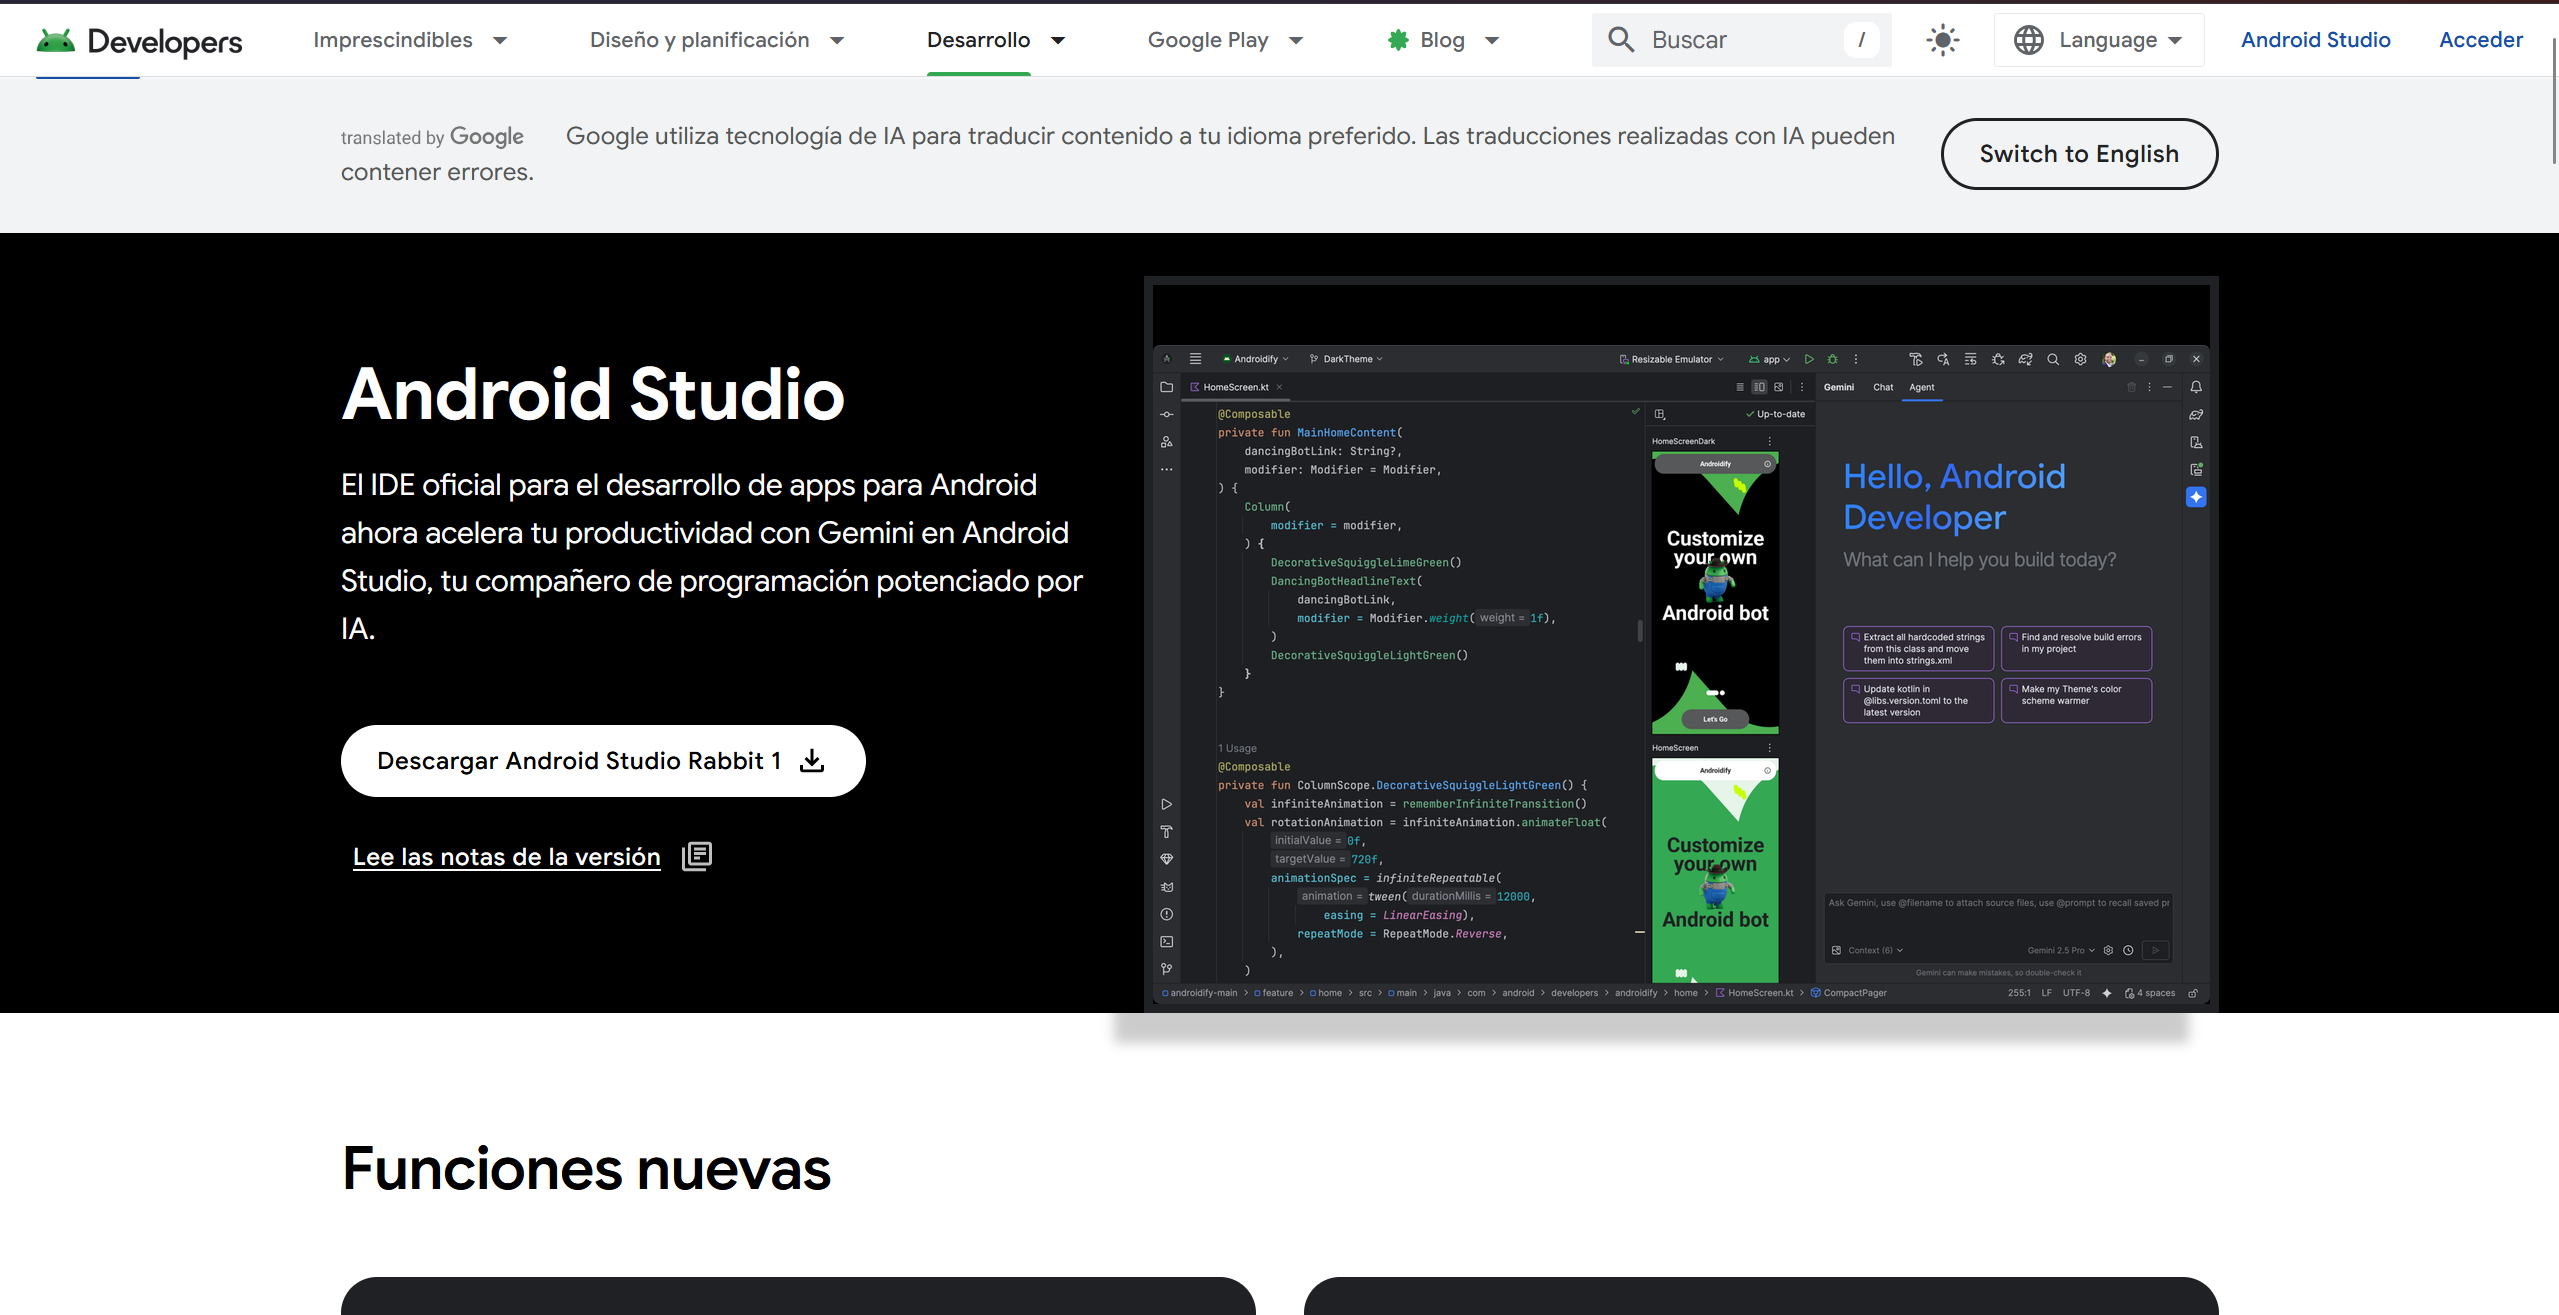
\includegraphics[width=1\linewidth]{figs/Descarga_AS_Rabbit1}}
	\caption{Instalador de Android Studio (Rabbit 1)}
	\label{fig:descargaasrabbit1}
\end{figure}
	\end{itemize}
	
	\campo{Paso 2 --- Ejecutar el instalador.}
	\begin{itemize}[leftmargin=*,itemsep=0.15em]
		\item \textbf{Windows}: doble clic en el \archivo{.exe} y seguir el asistente.
		\item \textbf{macOS}: abrir el \archivo{.dmg} y \textbf{arrastrar el icono a Aplicaciones}.
		\item \textbf{Linux}: descomprimir en \archivo{/opt/} y lanzar \archivo{android-studio/bin/studio}.
	\end{itemize}
	
	\begin{figure}[H]
		\centering
		\setlength{\fboxsep}{6pt}
		\setlength{\fboxrule}{1pt}
		\fbox{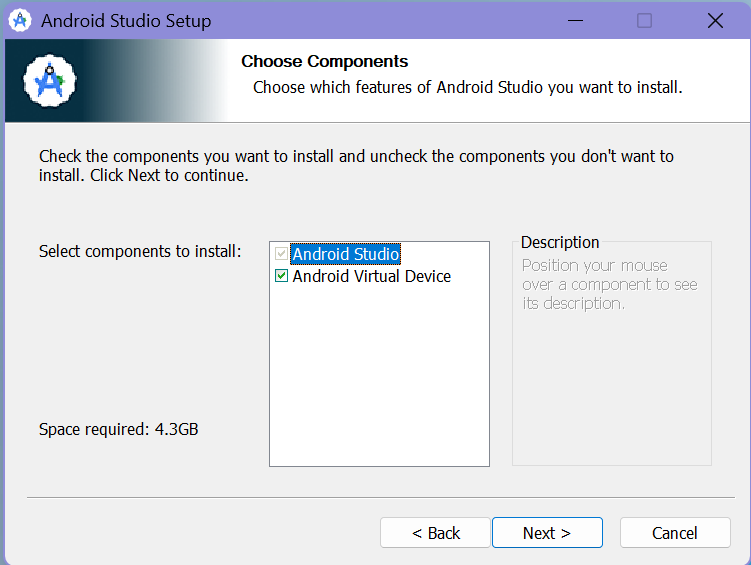
\includegraphics[width=0.65\linewidth]{figs/Instalacion_AS_1}}
		\caption{Instalador de Android Studio en Windows: pantalla \emph{Choose Components}, con \textbf{Android Studio} y \textbf{Android Virtual Device} marcados (4,3 GB de espacio necesario).}
		\label{fig:inst-componentes}
	\end{figure}

	\begin{figure}[H]
		\centering
		\setlength{\fboxsep}{6pt}
		\setlength{\fboxrule}{1pt}
		\fbox{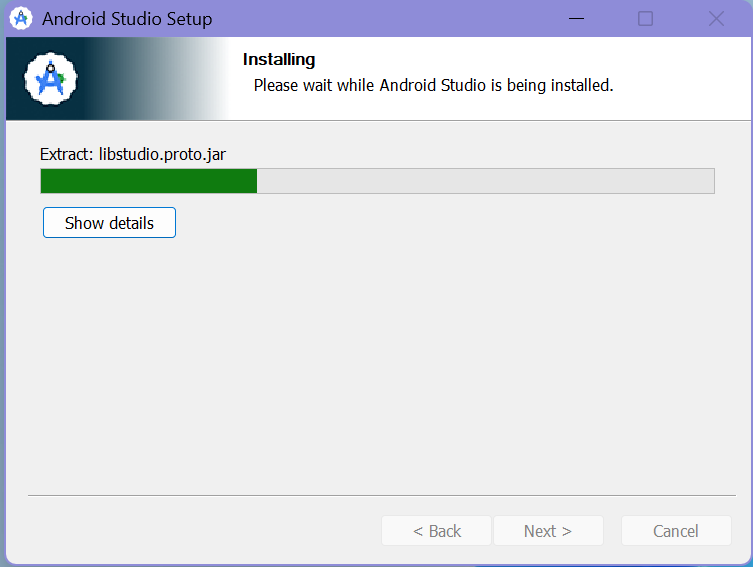
\includegraphics[width=0.65\linewidth]{figs/Instalacion_AS_2}}
		\caption{Instalador de Android Studio copiando los archivos (pantalla \emph{Installing}).}
		\label{fig:inst-progreso}
	\end{figure}

	\begin{figure}[H]
		\centering
		\setlength{\fboxsep}{6pt}
		\setlength{\fboxrule}{1pt}
		\fbox{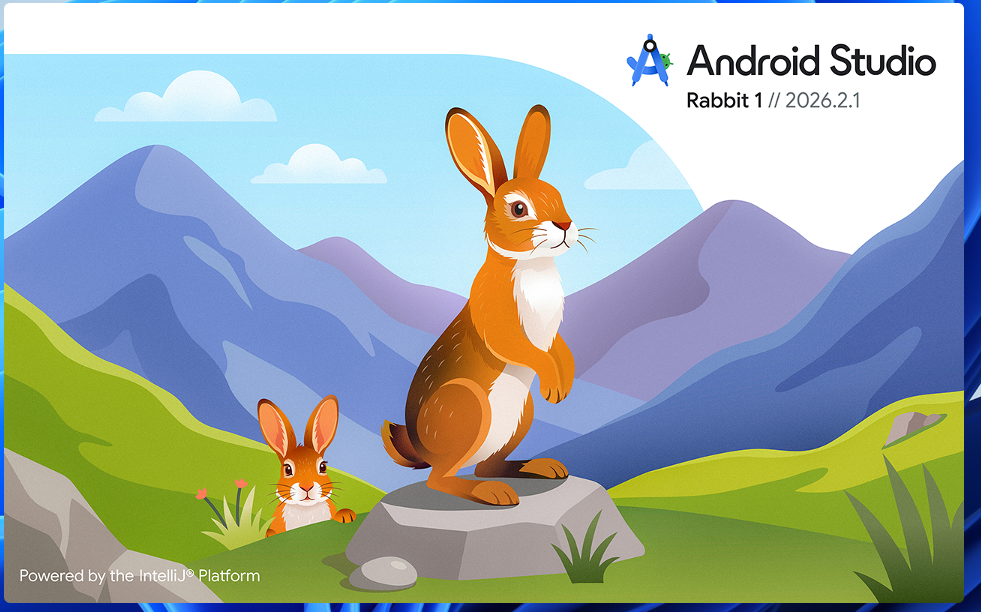
\includegraphics[width=0.8\linewidth]{figs/Instalacion_AS_3}}
		\caption{Pantalla de arranque de Android Studio Rabbit 1 (2026.2.1), que confirma la versión instalada.}
		\label{fig:arranque}
	\end{figure}

	\campo{Paso 3 --- El asistente de configuración inicial (Setup Wizard).}
	El asistente ofrece dos modos de instalación:
	\begin{itemize}[leftmargin=*,itemsep=0.15em]
		\item \textbf{Standard (estándard)}: instala automáticamente el conjunto recomendado.
		\item \textbf{Custom (personalizado)}: permite elegir componente a componente.
	\end{itemize}
	
	\begin{figure}[H]
		\centering
		\setlength{\fboxsep}{6pt}
		\setlength{\fboxrule}{1pt}
		\fbox{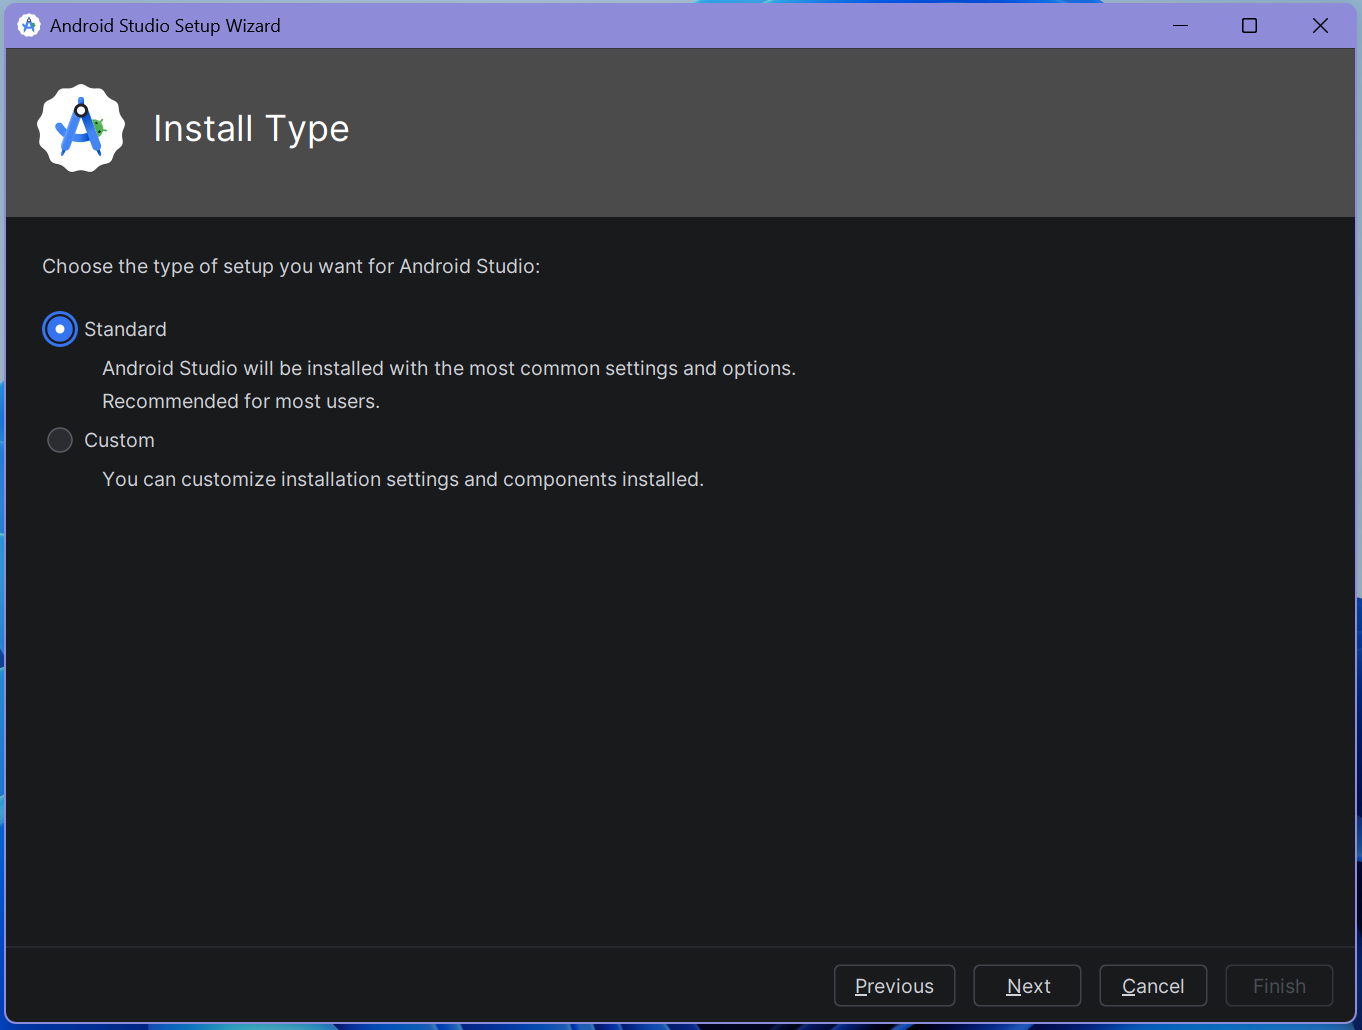
\includegraphics[width=1\linewidth]{figs/Instalacion_AS_4}}
		\caption{Asistente de configuración inicial (\emph{Setup Wizard}): pantalla \emph{Install Type} con el modo \textbf{Standard} seleccionado.}
		\label{fig:wizard-tipo}
	\end{figure}

	\begin{figure}[H]
		\centering
		\setlength{\fboxsep}{6pt}
		\setlength{\fboxrule}{1pt}
		\fbox{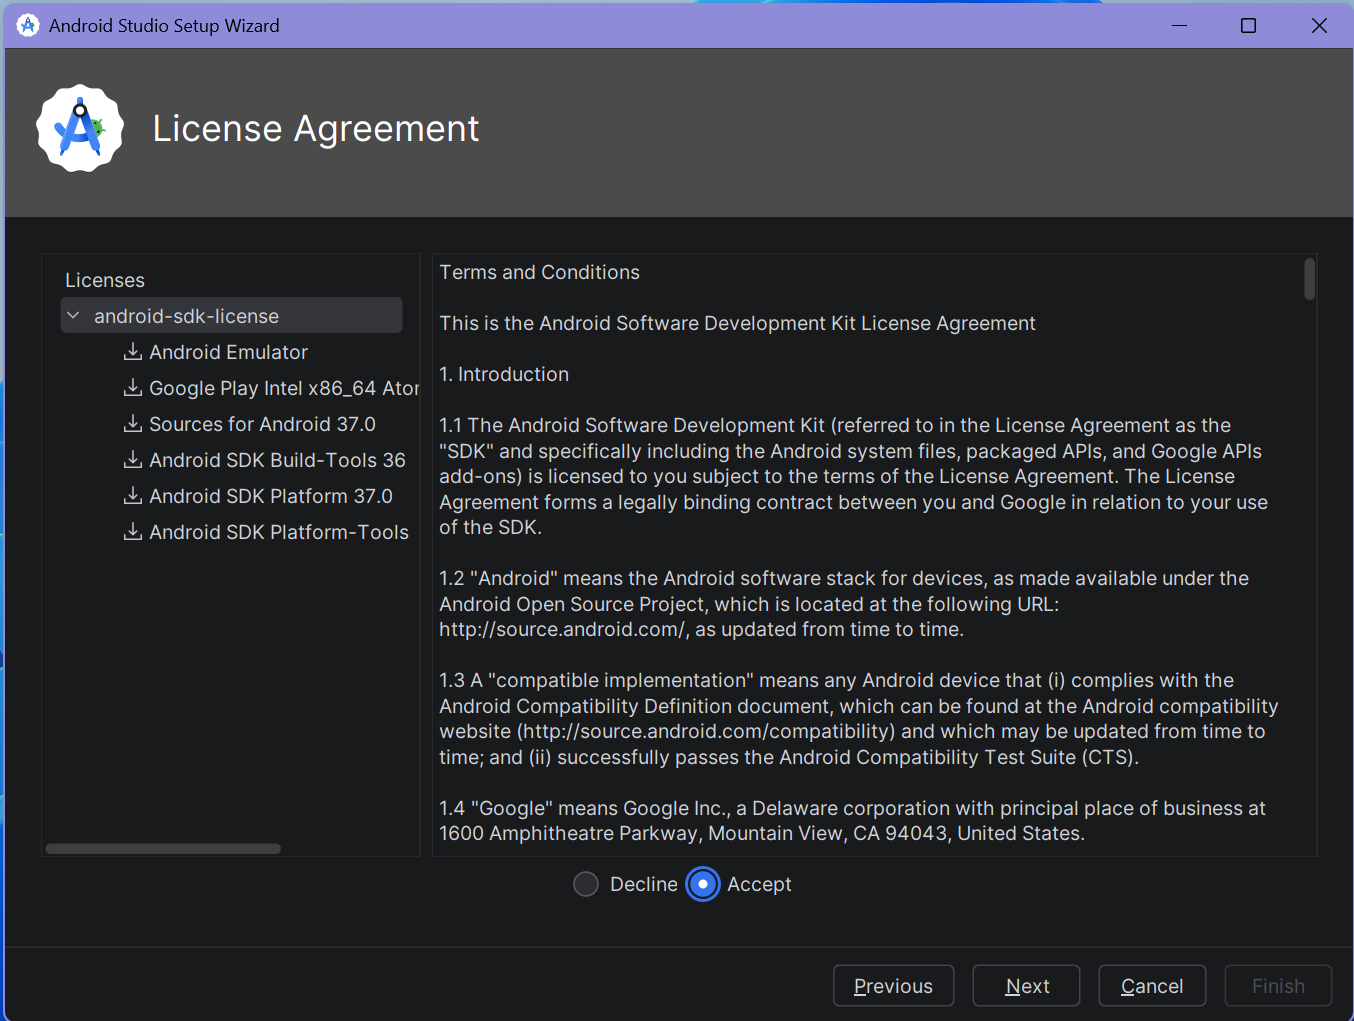
\includegraphics[width=1\linewidth]{figs/Instalacion_AS_5}}
		\caption{\emph{Setup Wizard}: aceptación de la licencia \texttt{android-sdk-license}, que cubre los componentes del SDK que se van a descargar (emulador, imagen del sistema, fuentes, \emph{Build-Tools}, \emph{Platform} y \emph{Platform-Tools}).}
		\label{fig:wizard-licencia}
	\end{figure}

	\begin{figure}[H]
		\centering
		\setlength{\fboxsep}{6pt}
		\setlength{\fboxrule}{1pt}
		\fbox{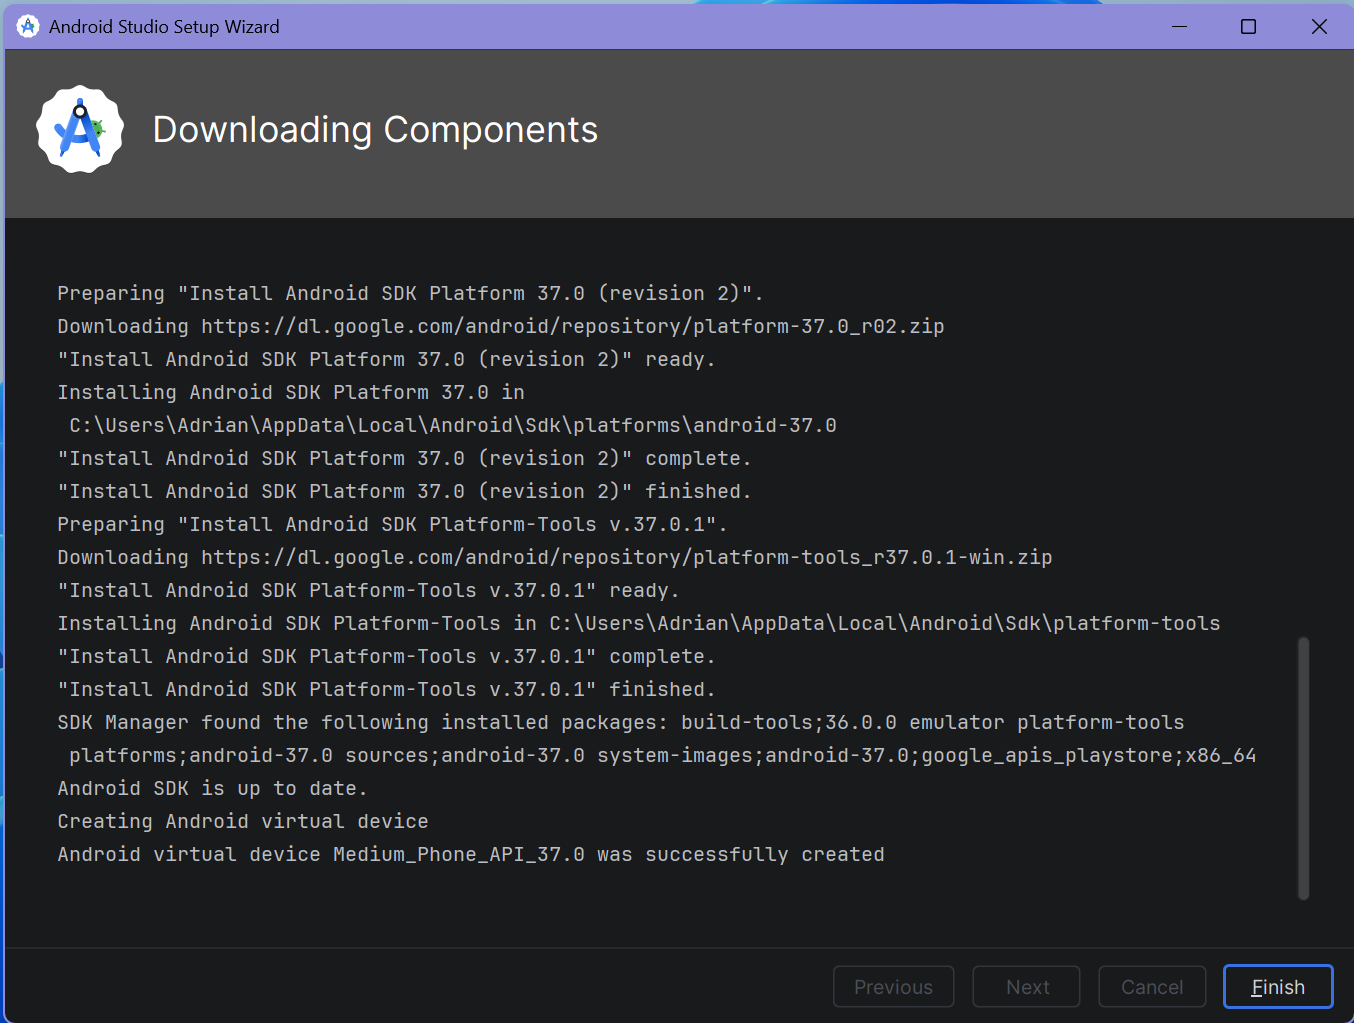
\includegraphics[width=1\linewidth]{figs/Instalacion_AS_6}}
		\caption{\emph{Setup Wizard}: descarga de componentes terminada. El registro indica que el SDK está actualizado y que se ha creado el dispositivo virtual \texttt{Medium\_Phone\_API\_37.0}.}
		\label{fig:wizard-descarga}
	\end{figure}

	
	\begin{figure}[H]
		\centering
		\setlength{\fboxsep}{6pt}
		\setlength{\fboxrule}{1pt}
		\fbox{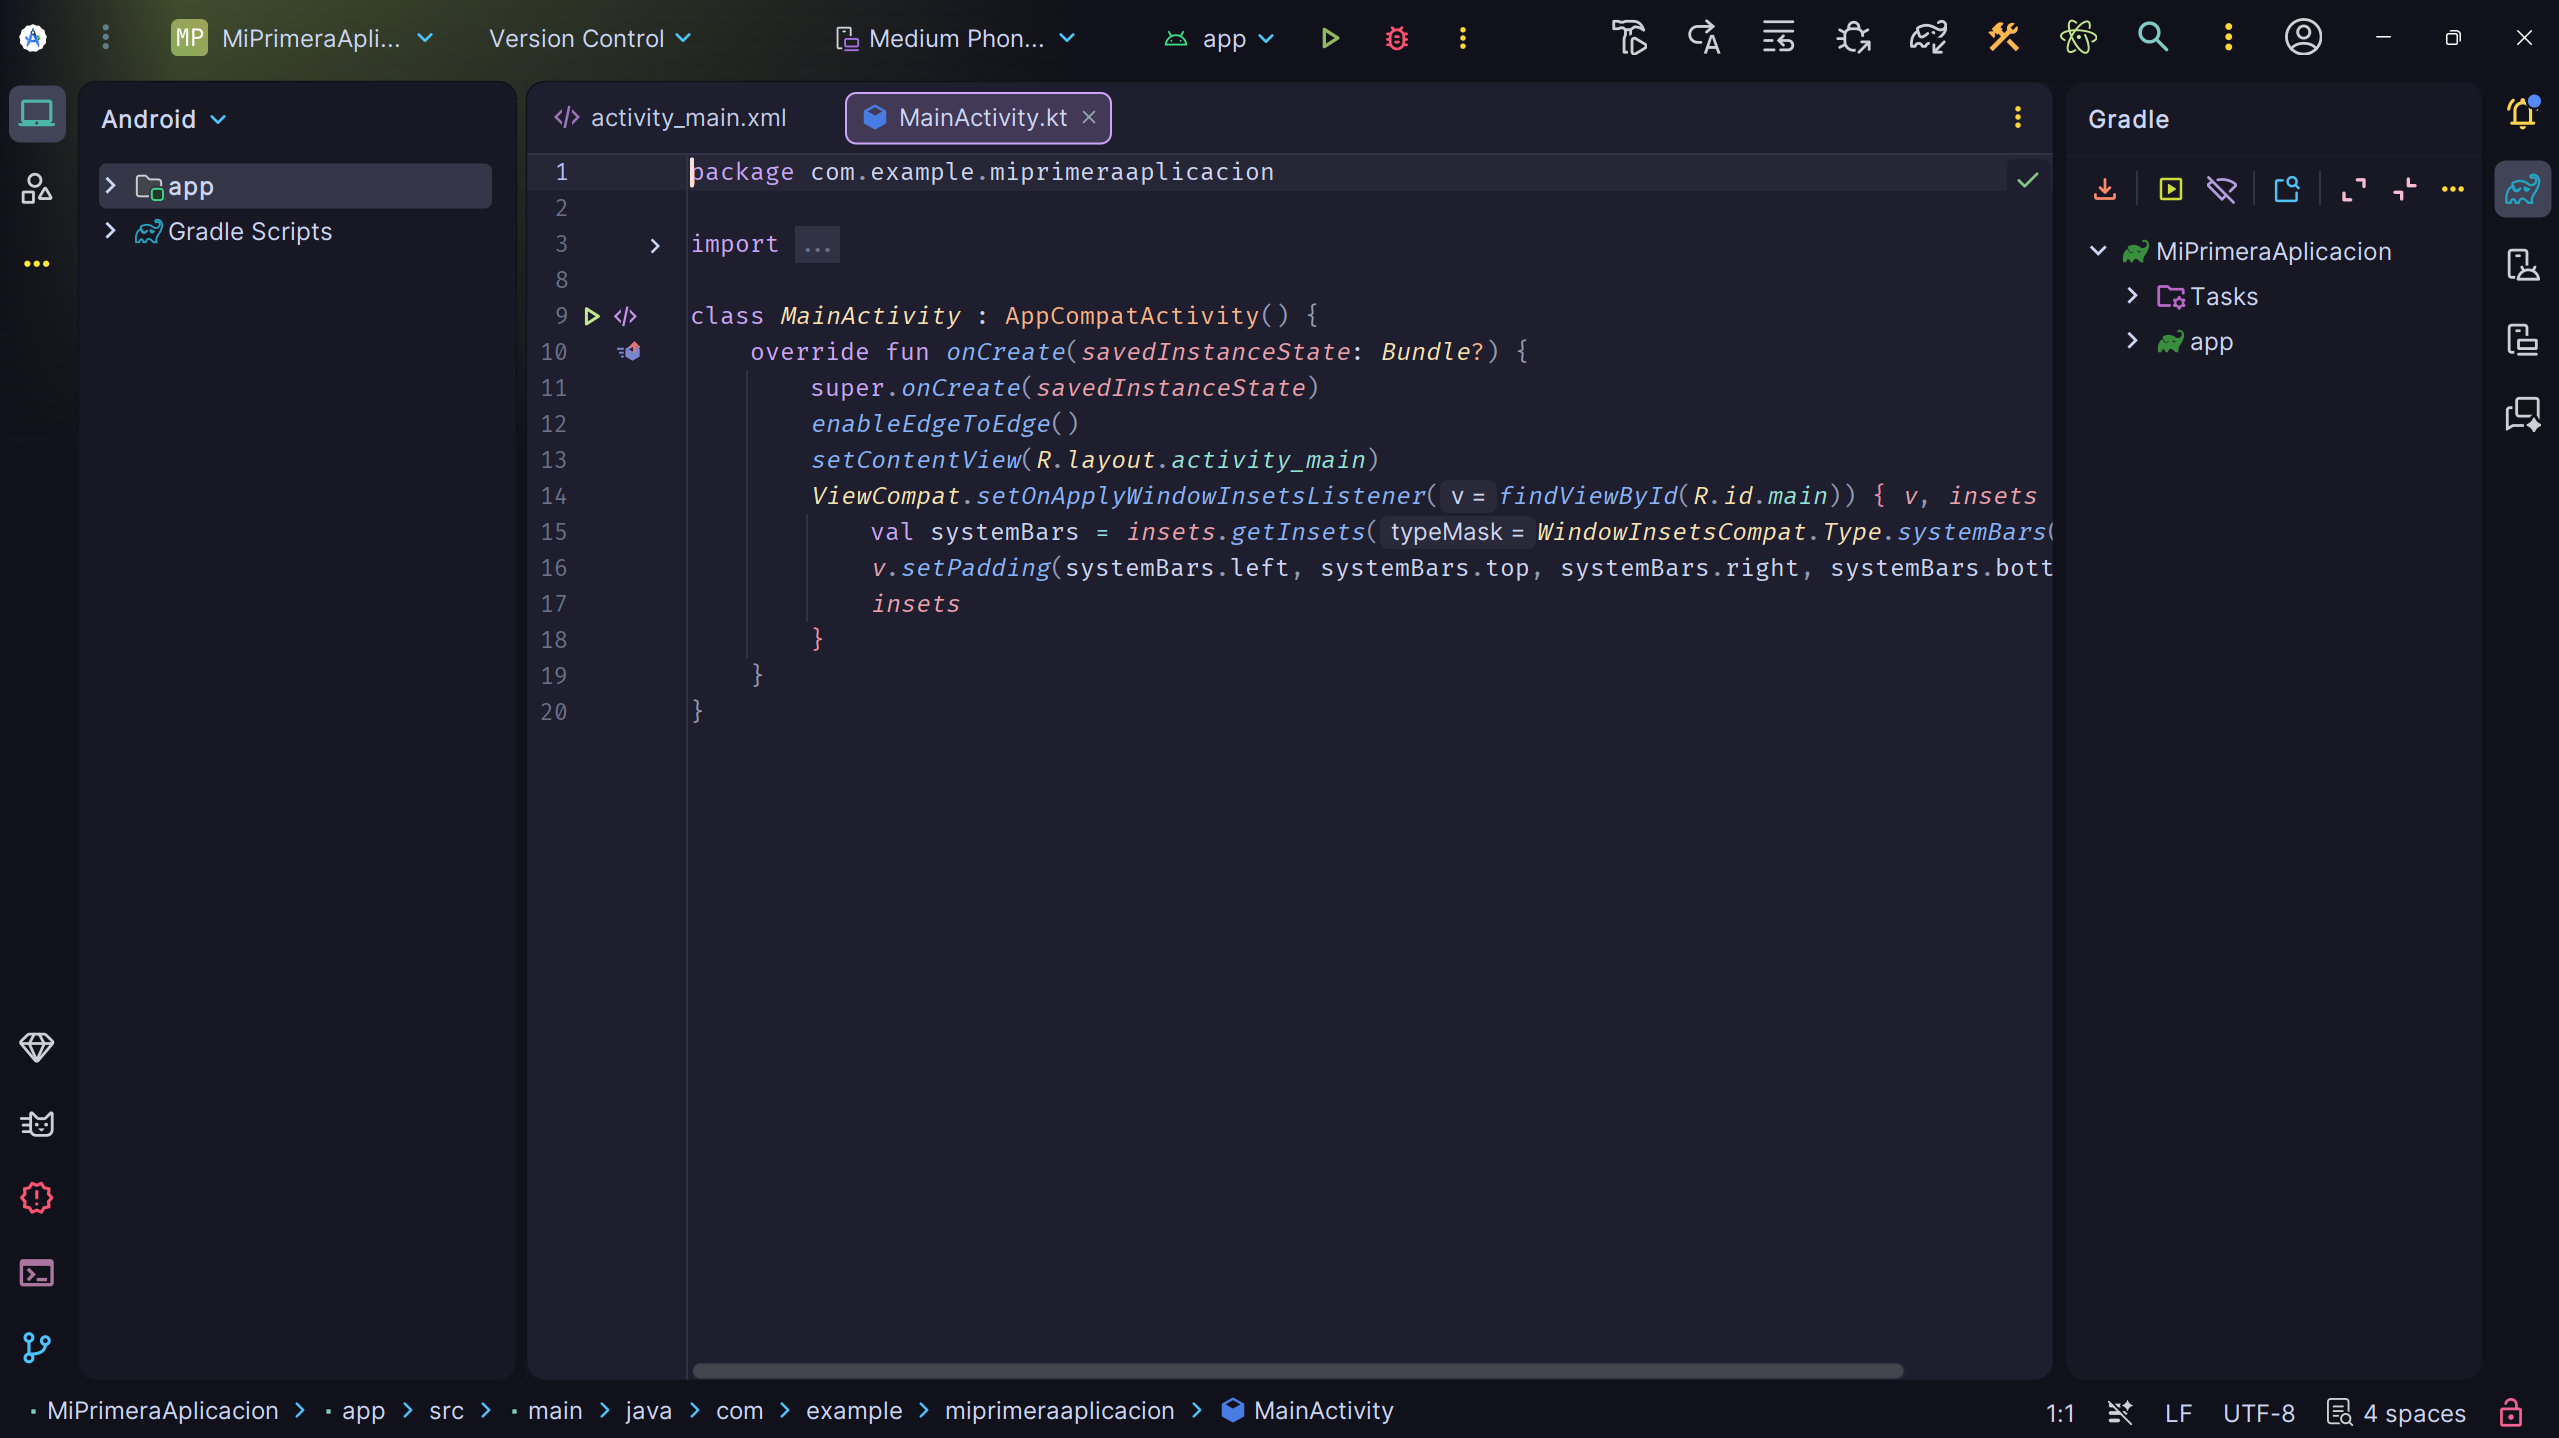
\includegraphics[width=1\linewidth]{figs/AndroidStudio_1}}
		\caption{Pantalla principal de Android Studio con el proyecto \texttt{MiPrimeraAplicacion} abierto: panel \emph{Project} a la izquierda, editor en el centro y panel de Gradle a la derecha.}
		\label{fig:pantalla-principal}
	\end{figure}

	
	\subsection{Creación de un proyecto de prueba}
	
	\campo{Paso 1 --- Abrir el asistente de nuevo proyecto.}
	Botón \textbf{New Project} en la pantalla de bienvenida, o \textbf{File > New > New Project}.
	
	\campo{Paso 2 --- Elegir la plantilla.}
	En el panel de plantillas, dentro de \textbf{Phone and Tablet}, hay que seleccionar \textbf{\texttt{Empty Views Activity}}.

	\begin{figure}[H]
		\centering
		\setlength{\fboxsep}{6pt}
		\setlength{\fboxrule}{1pt}
		\fbox{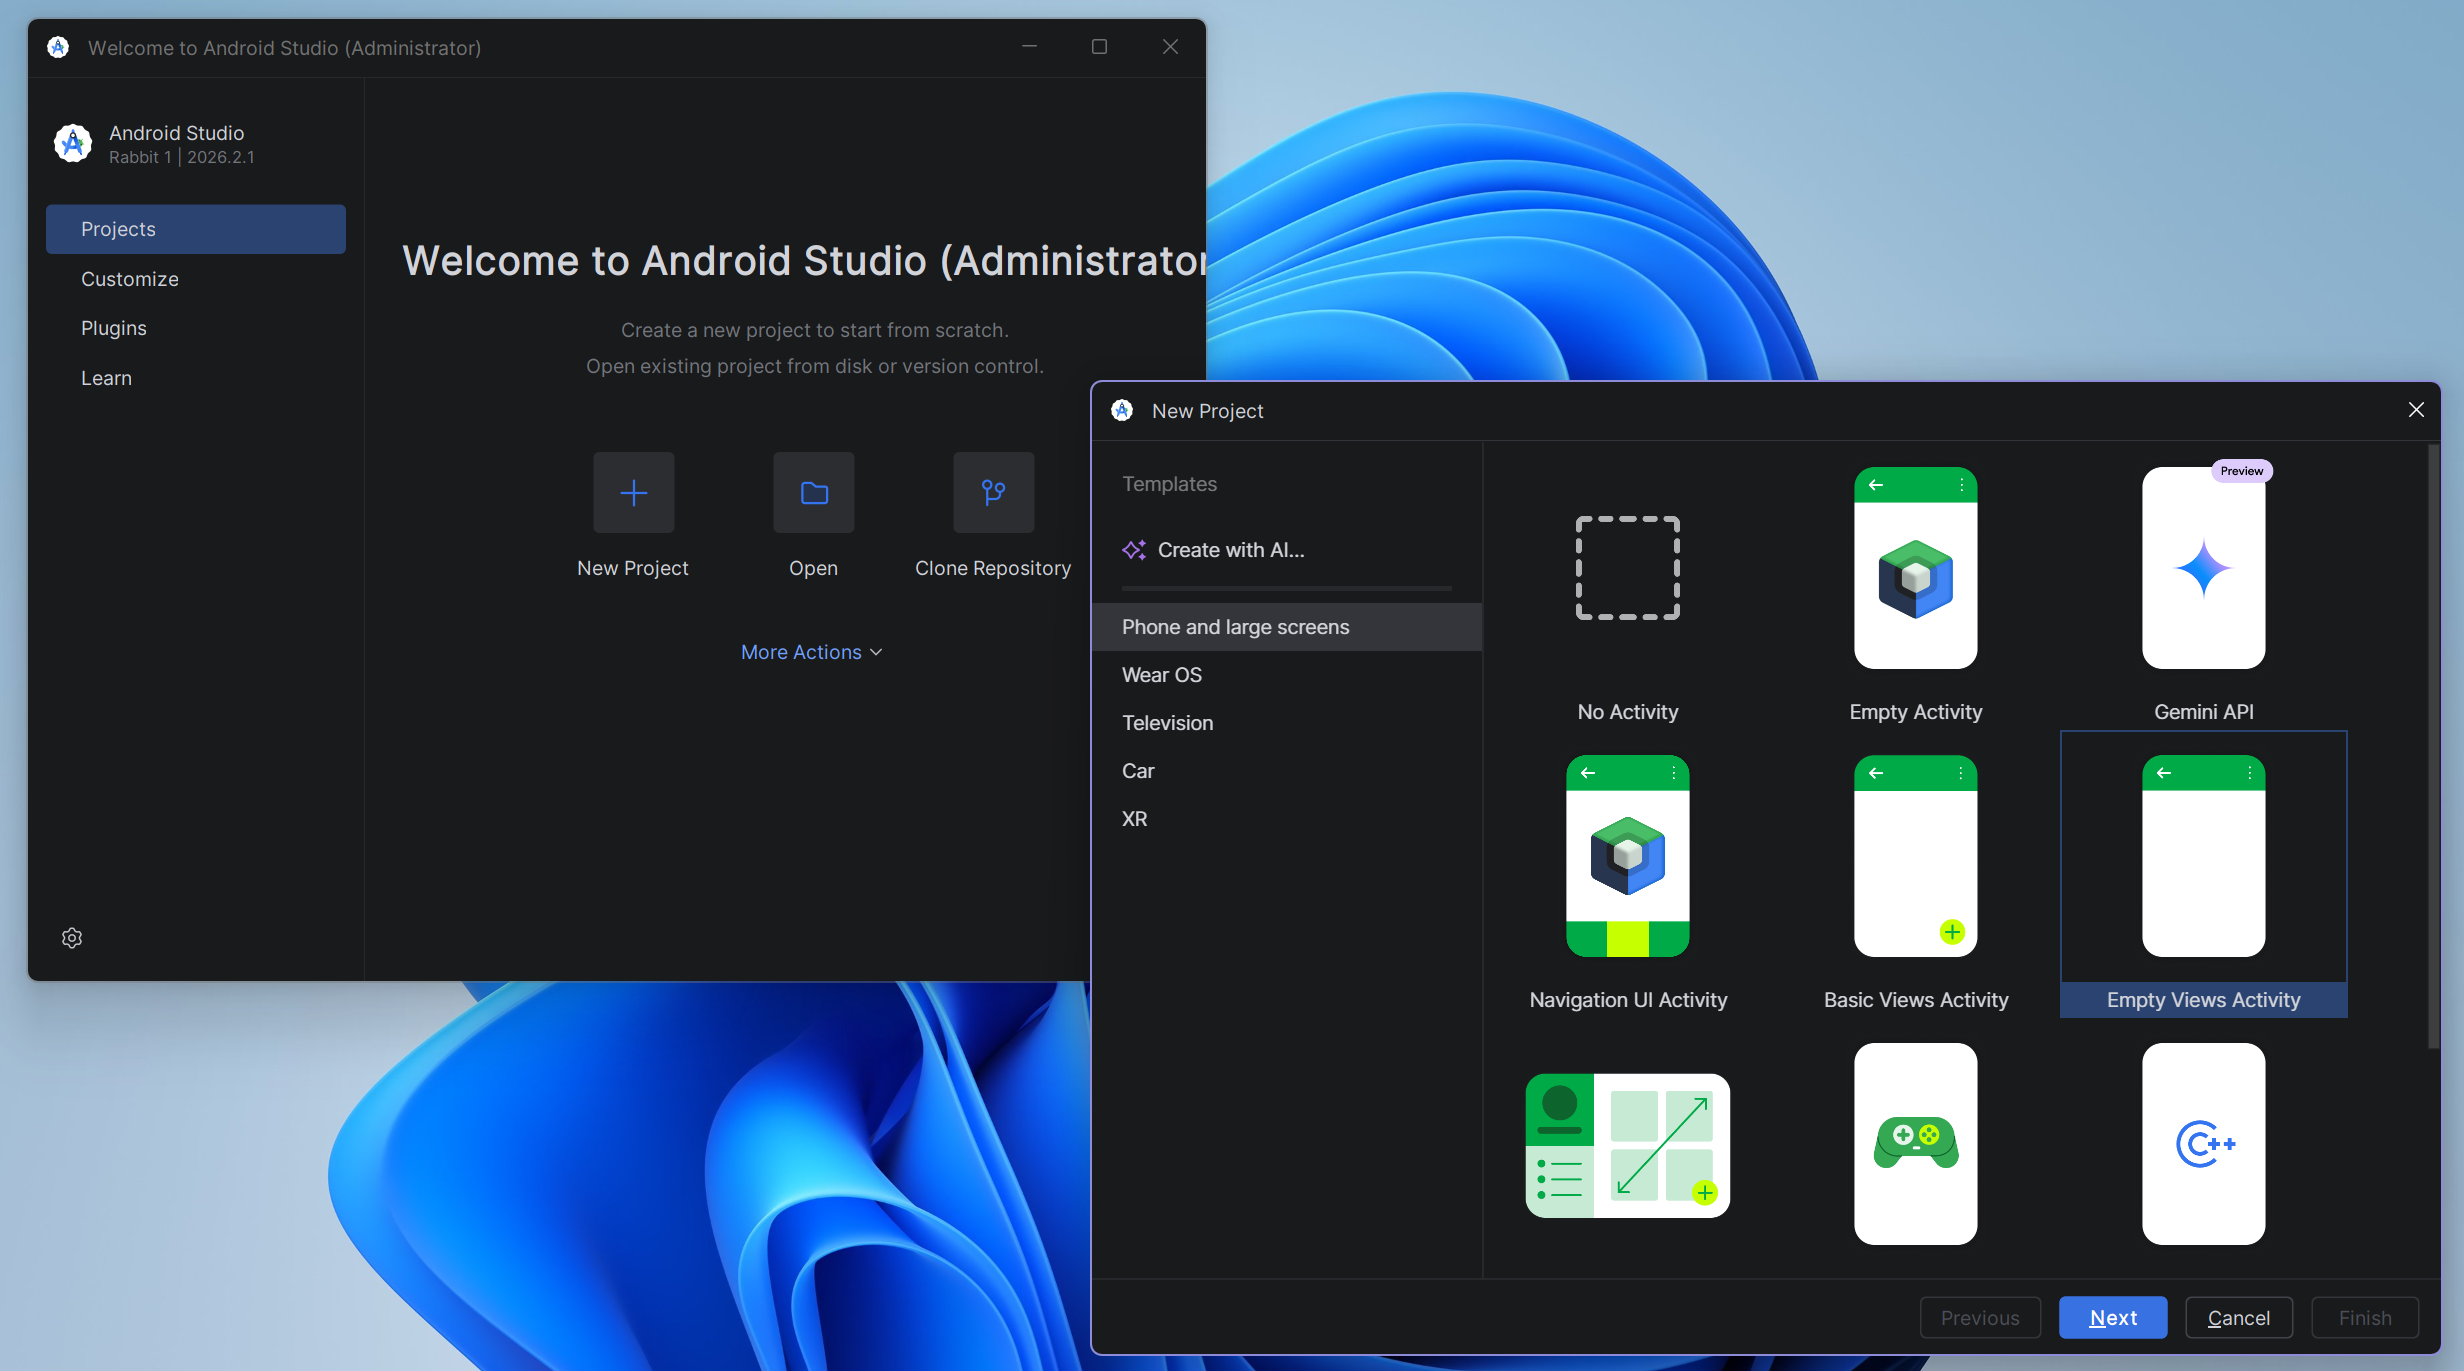
\includegraphics[width=1\linewidth]{figs/Creacion_PrimerProyecto_1}}
		\caption{Asistente \emph{New Project}: plantilla \textbf{Empty Views Activity} seleccionada en la categoría \emph{Phone and large screens}.}
		\label{fig:plantilla}
	\end{figure}

	
	\begin{warnbox}
		\textbf{\color{accent!80!black}\faExclamationTriangle\ \ Ojo con la plantilla.}
		En Android Studio conviven dos plantillas que se parecen mucho y elegir la equivocada cambia todo lo que viene después:
		\begin{itemize}[leftmargin=*,itemsep=0.15em]
			\item \textbf{\texttt{Empty Views Activity}} \flecha genera la interfaz con \textbf{vistas XML} en \archivo{res/layout/}.
			\item \textbf{\texttt{Empty Activity}} \flecha genera la interfaz con \textbf{Jetpack Compose}, sin ningún XML.
		\end{itemize}
		El enunciado pide la de vistas XML, así que esa es la que uso. Aun así, desde mayo de 2026 la posición oficial de Android Developers es que el desarrollo de interfaces en Android es \enquote{Compose-first}, así que el sistema de vistas que nos piden aquí ya está en mantenimiento.
	\end{warnbox}
	
	\campo{Paso 3 --- Configurar el proyecto.}
	
	\begin{table}[htbp]
		\centering
		\small
		\begin{tabularx}{\textwidth}{@{}>{\RaggedRight\arraybackslash}p{3cm} >{\RaggedRight\arraybackslash}p{5cm} >{\RaggedRight\arraybackslash}X@{}}
			\toprule
			\rowcolor{primary}
			\textcolor{white}{\sffamily\bfseries Campo} & \textcolor{white}{\sffamily\bfseries Valor a introducir} & \textcolor{white}{\sffamily\bfseries Por qué} \\
			\midrule
			\textbf{Name} & \archivo{PracticaEntornoMovil} & Nombre del proyecto y de la carpeta \\
			\rowcolor{soft}
			\textbf{Package name} & \archivo{com.ejemplo.practicaentornomovil} & Identificador único. No se puede cambiar después \\
			\textbf{Save location} & Carpeta con espacio & El proyecto + emulador se llevan bastante \\
			\rowcolor{soft}
			\textbf{Language} & \textbf{Kotlin} & El enunciado es explícito: debe ser Kotlin, no Java \\
			\textbf{Minimum API level} & \textbf{API 24 (Android 7.0 Nougat)} & Valor que usa el codelab oficial de Google \\
			\bottomrule
		\end{tabularx}
		\caption{Campos de configuración del nuevo proyecto}
	\end{table}
	
	\begin{warnbox}
		\textbf{\color{accent!80!black}\faExclamationTriangle\ \ Sobre una contradicción del enunciado.}
		En el punto 3.4 aparece \enquote{la selección de Java}, mientras que en el 3.2 se dice explícitamente que el proyecto debe ser en Kotlin, no en Java. Es una errata y lo dejo escrito aquí porque me parece que conviene subirlo. Yo me quedo con \textbf{Kotlin}, que además es el lenguaje oficial desde 2019, y por eso el archivo se llama \archivo{MainActivity.kt} y no \archivo{MainActivity.java}.
	\end{warnbox}
	
	\begin{figure}[H]
		\centering
		\setlength{\fboxsep}{6pt}
		\setlength{\fboxrule}{1pt}
		\fbox{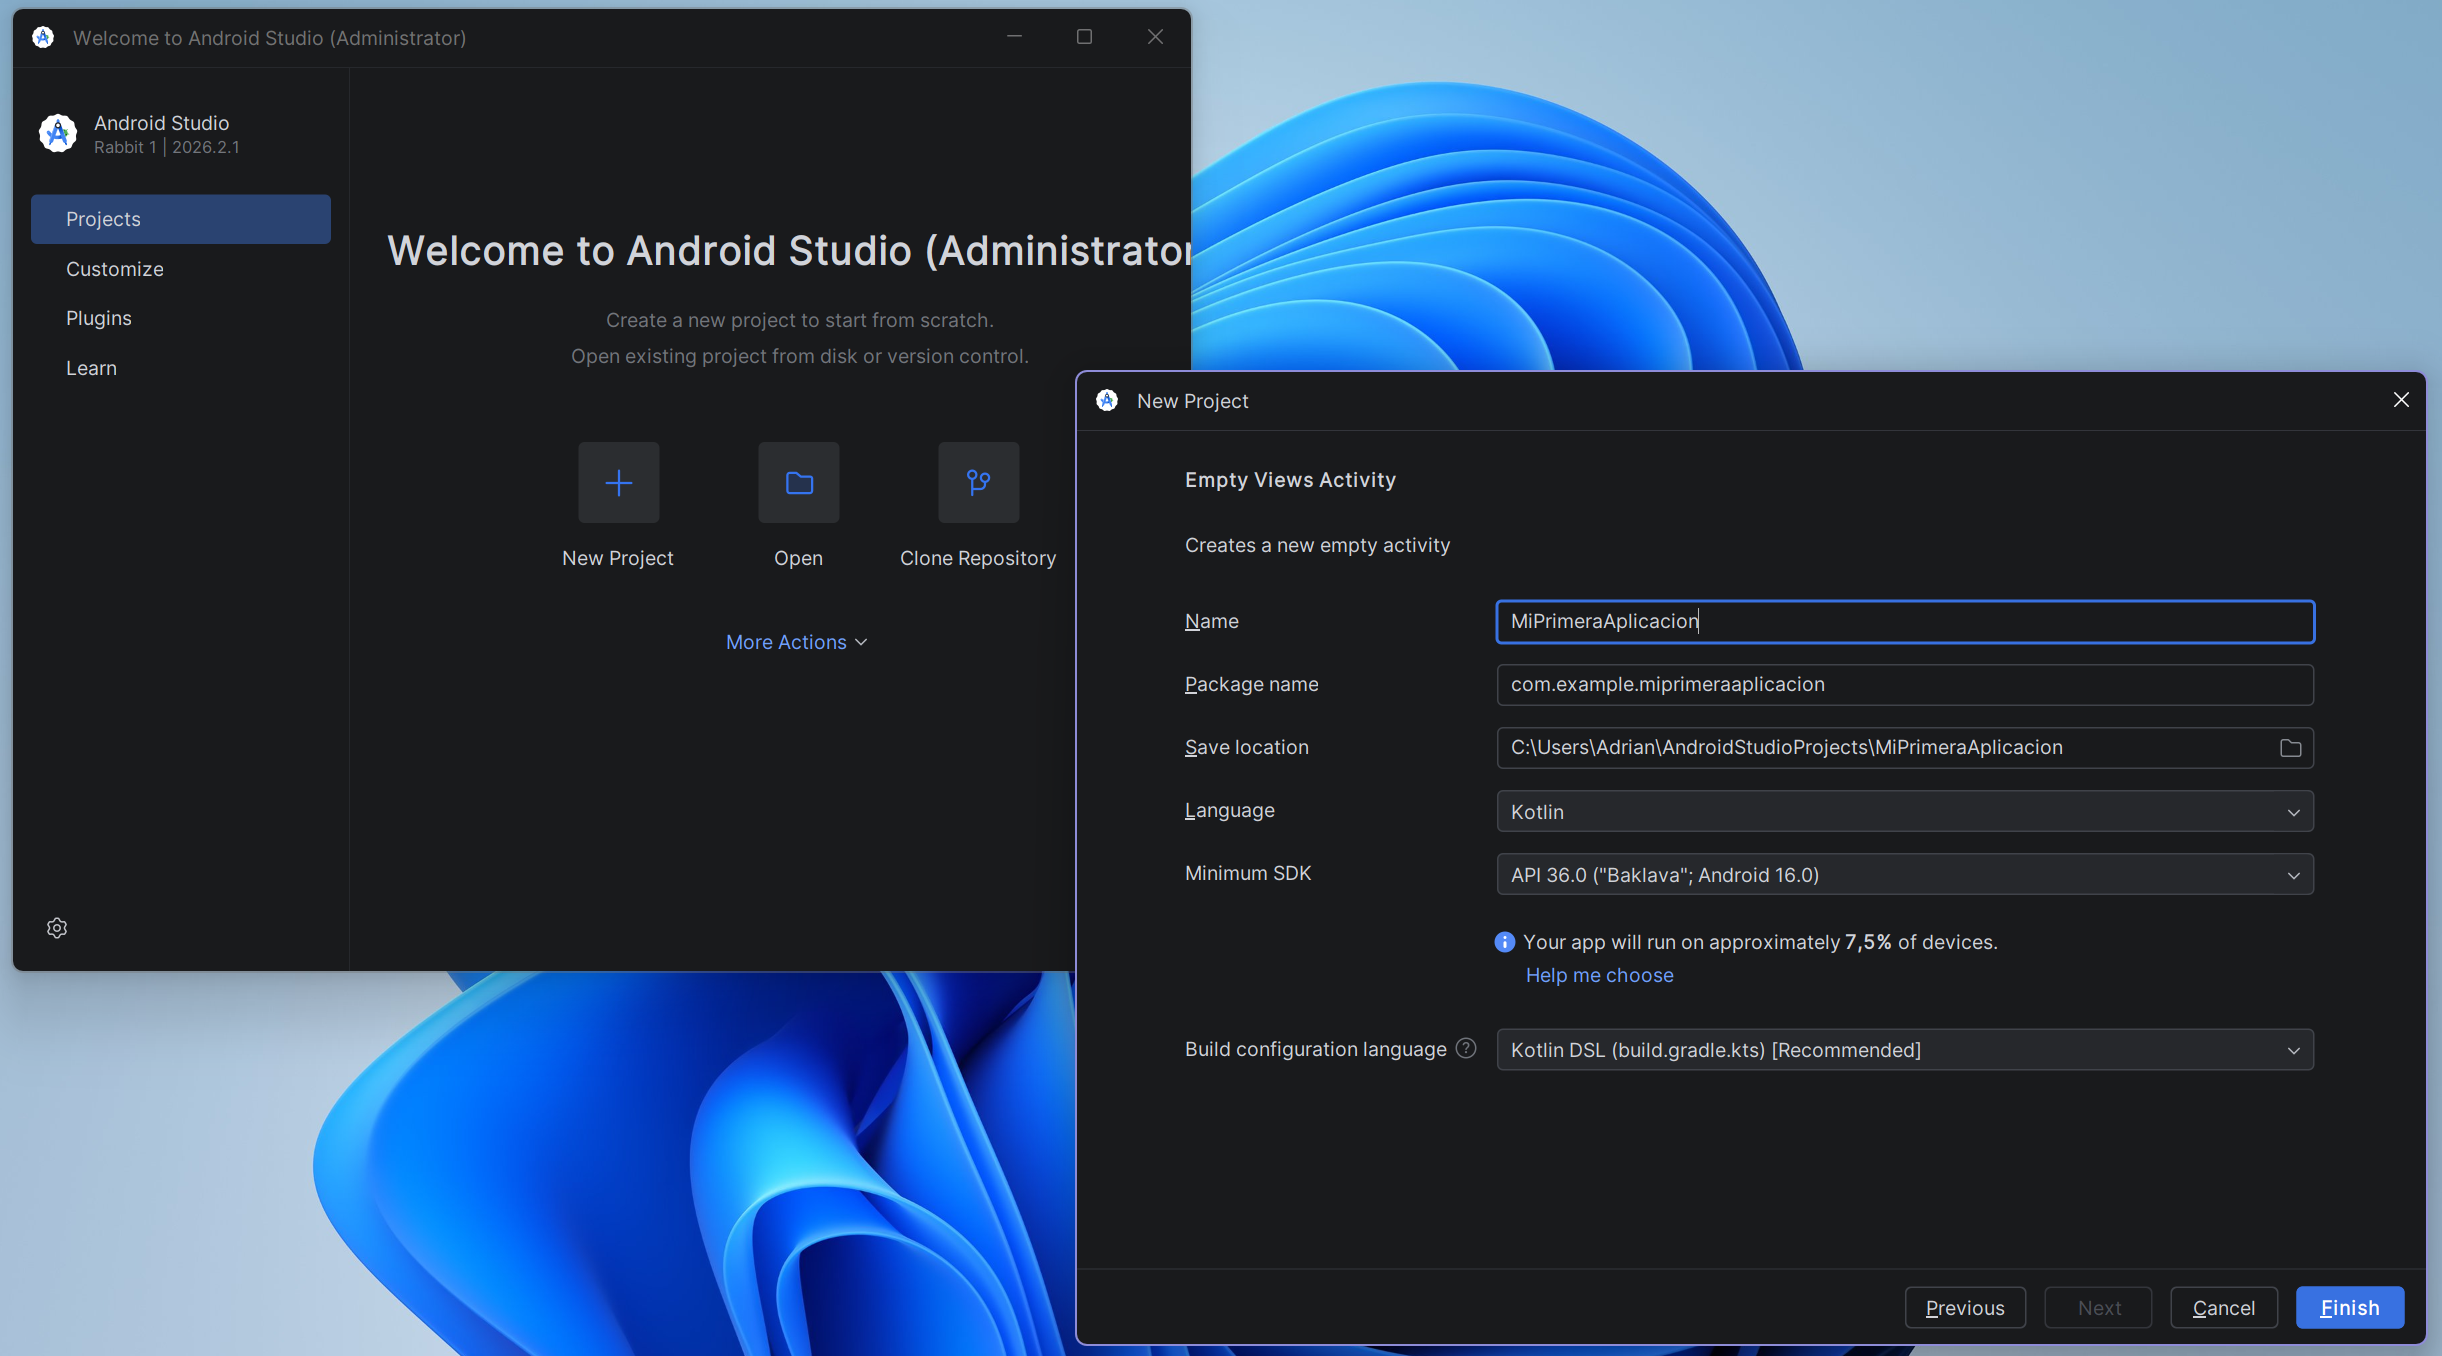
\includegraphics[width=1\linewidth]{figs/Creacion_PrimerProyecto_2}}
		\caption{Asistente \emph{New Project} con los campos rellenos: nombre \texttt{MiPrimeraAplicacion}, \textbf{Language = Kotlin} y SDK mínimo API 36.}
		\label{fig:nuevo-proyecto}
	\end{figure}

	
	\campo{Paso 4 --- Esperar a la sincronización.}
	Al pulsar \textbf{Finish}, Android Studio crea el proyecto y lanza una sincronización de Gradle en segundo plano. En la parte inferior se ve la barra de progreso, y conviene esperar a que termine antes de tocar nada más.
	
	\figpend{3.5}{Captura de la barra inferior de Android Studio con la tarea de Gradle en curso, o ya completada y sin errores en rojo.}
	
	\subsection{Comprobación del funcionamiento}
	
	\campo{Paso 1 --- Localizar la estructura del proyecto.}
	Nada más abrir el proyecto, lo primero que hago es mirar el árbol de archivos, que es donde se ve si Android Studio ha generado lo que se le ha pedido:
	
	\begin{verbatim}
		PracticaEntornoMovil/
		|-- app/
		|   |-- build.gradle.kts
		|   |-- proguard-rules.pro
		|   `-- src/main/
		|       |-- AndroidManifest.xml
		|       |-- java/com/ejemplo/practicaentornomovil/
		|       |   `-- MainActivity.kt            <-- ACTIVIDAD PRINCIPAL
		|       `-- res/
		|           |-- layout/
		|           |   `-- activity_main.xml      <-- DISEÑO DE LA INTERFAZ
		|           |-- mipmap-anydpi-v26/
		|           |-- values/
		|           `-- xml/
		|-- build.gradle.kts
		|-- gradle.properties
		`-- settings.gradle.kts
	\end{verbatim}
	
	\campo{Paso 2 --- Identificar la actividad principal y el diseño.}
	Son los dos archivos que tengo que enseñar como evidencia, porque son los que demuestran que el proyecto está bien creado:
	
	\begin{table}[htbp]
		\centering
		\small
		\begin{tabularx}{\textwidth}{@{}>{\RaggedRight\arraybackslash}p{3.5cm} >{\RaggedRight\arraybackslash}p{5.5cm} >{\RaggedRight\arraybackslash}X@{}}
			\toprule
			\rowcolor{primary}
			\textcolor{white}{\sffamily\bfseries Archivo} & \textcolor{white}{\sffamily\bfseries Ruta} & \textcolor{white}{\sffamily\bfseries Qué contiene} \\
			\midrule
			\textbf{Actividad principal} & \archivo{app/src/main/java/.../MainActivity.kt} & La clase \code{MainActivity} y su \code{onCreate}, que llama a \code{setContentView} \\
			\rowcolor{soft}
			\textbf{Diseño} & \archivo{app/src/main/res/layout/activity\_main.xml} & El XML con la jerarquía de vistas \\
			\bottomrule
		\end{tabularx}
		\caption{Archivos principales del proyecto}
	\end{table}

	\begin{figure}[H]
		\centering
		\setlength{\fboxsep}{6pt}
		\setlength{\fboxrule}{1pt}
		\fbox{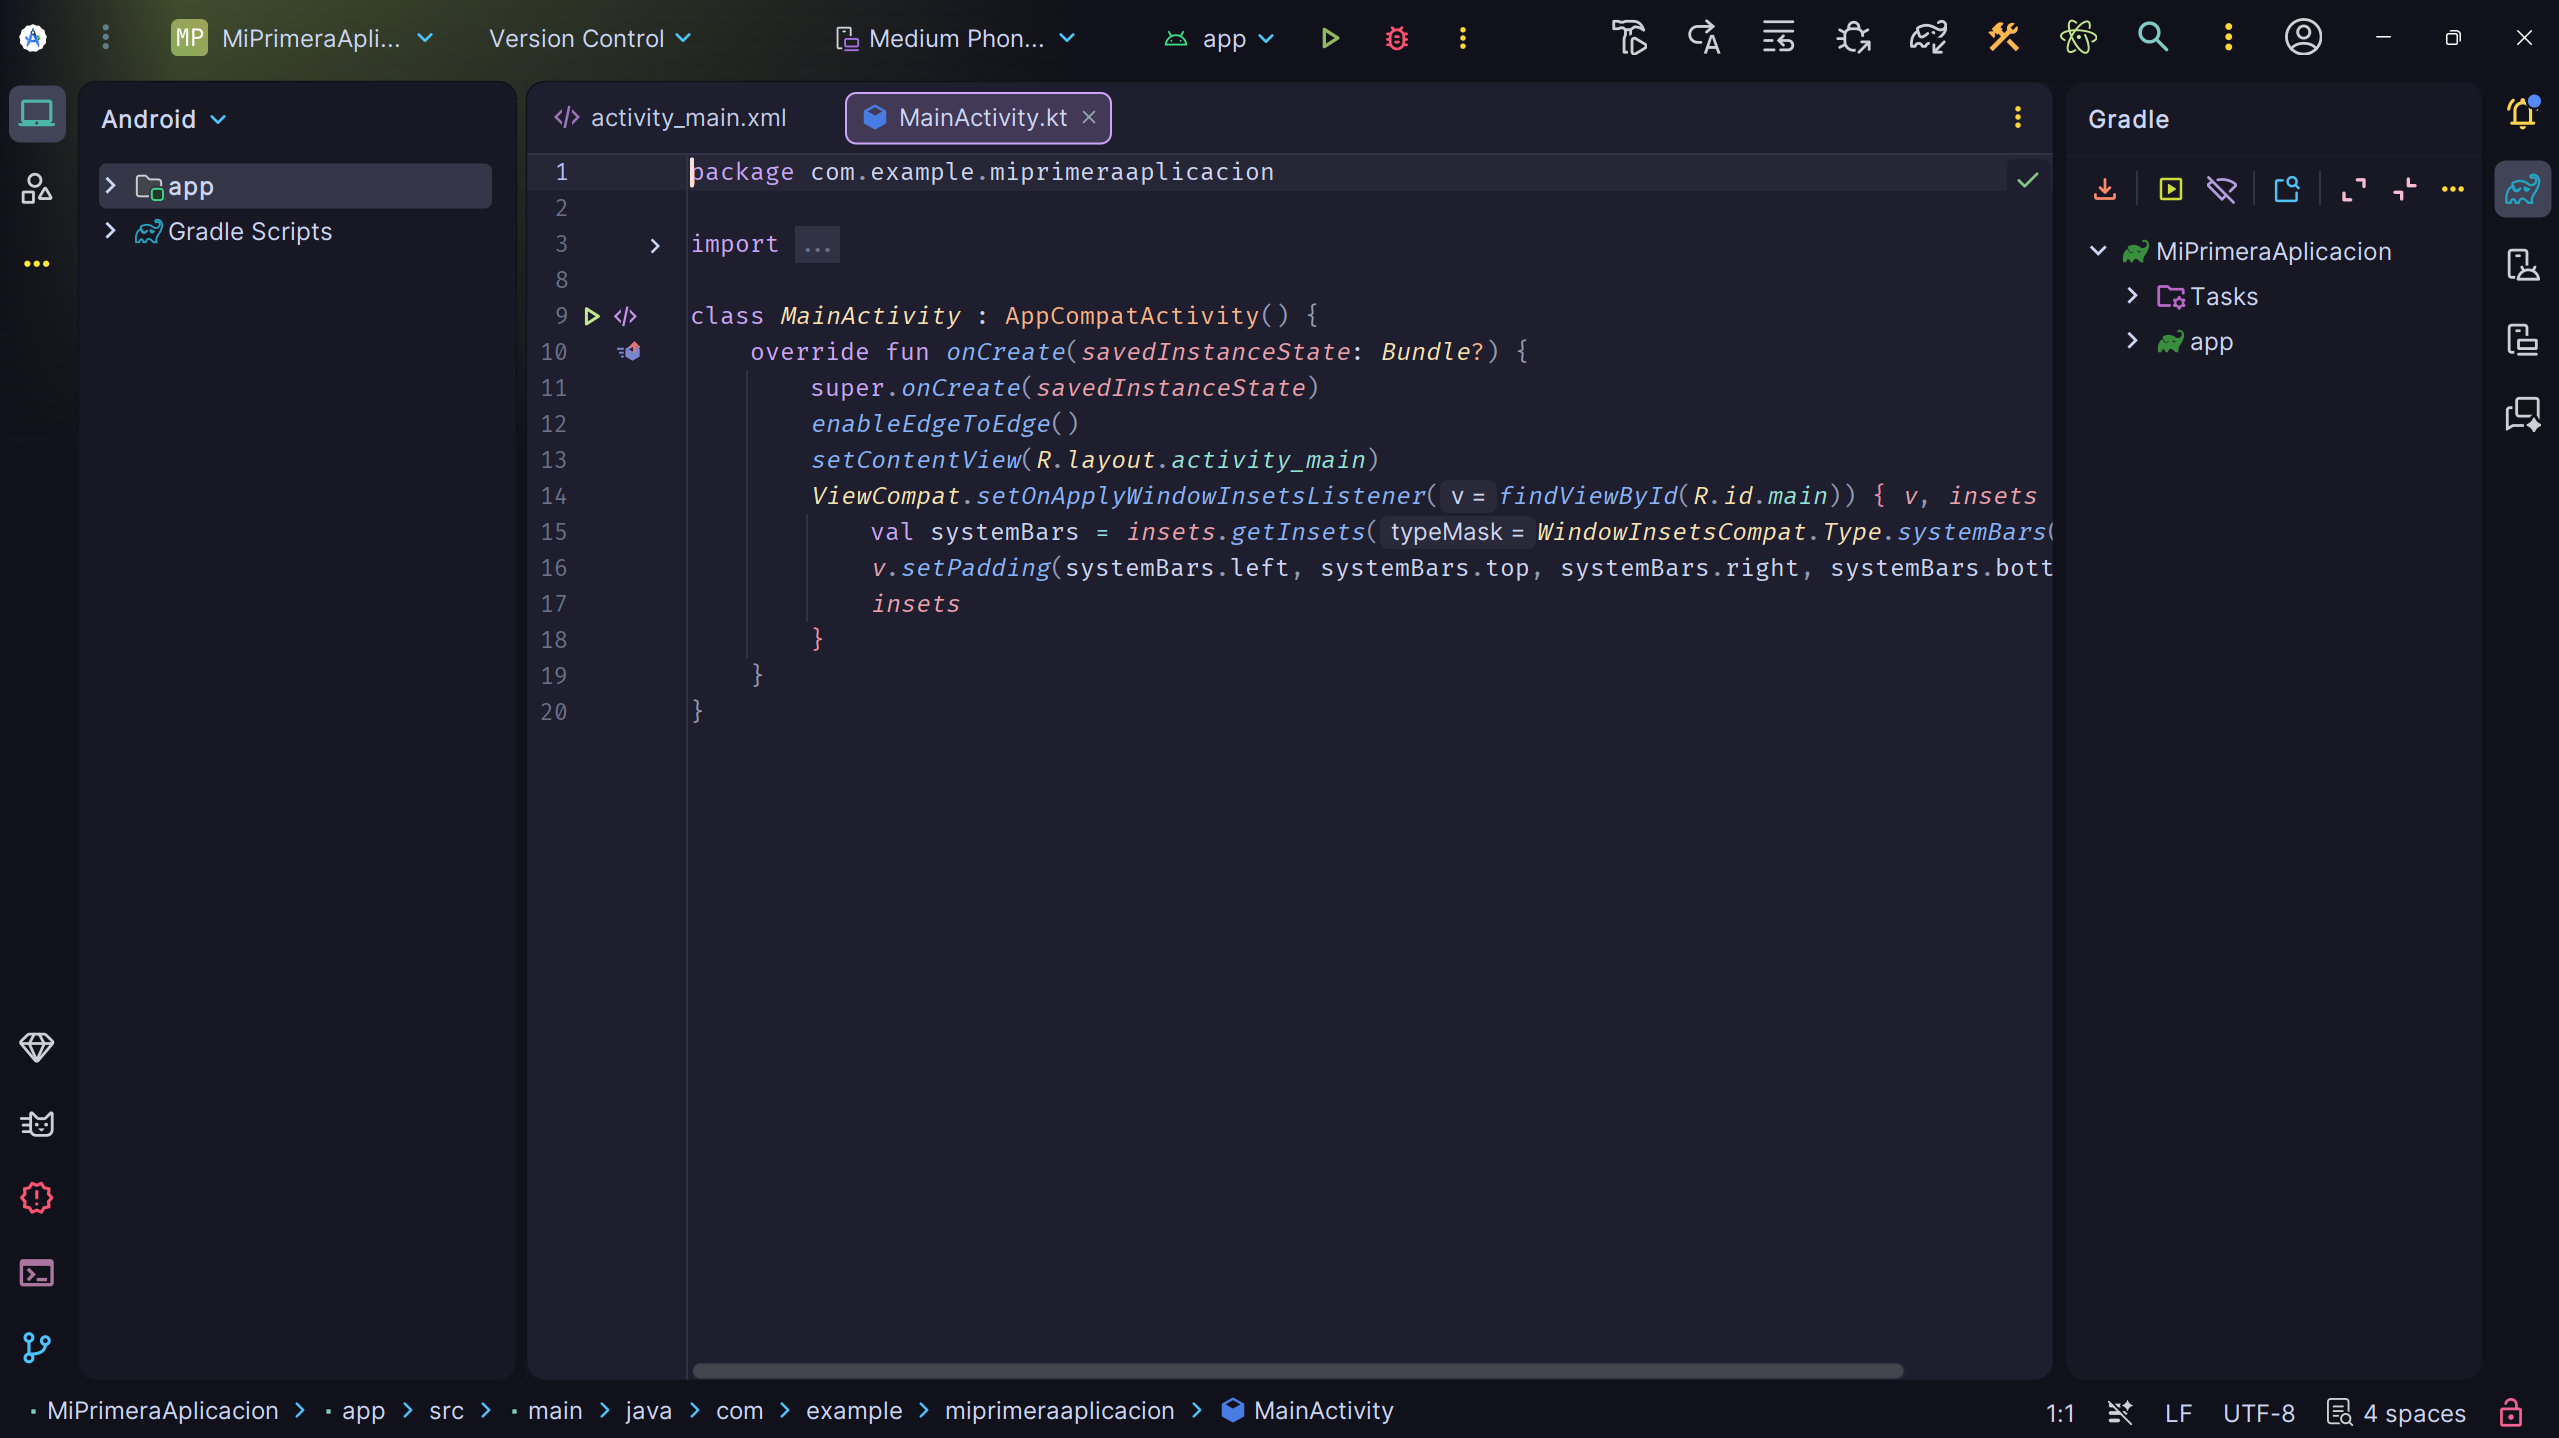
\includegraphics[width=1\linewidth]{figs/AndroidStudio_1}}
		\caption{Editor con el archivo \archivo{MainActivity.kt}: la extensión \archivo{.kt} y la declaración \code{class MainActivity : AppCompatActivity()} confirman que la actividad principal está escrita en Kotlin.}
		\label{fig:mainactivity}
	\end{figure}

	\figpend{3.7b}{Captura del archivo \archivo{activity\_main.xml} abierto (vista \emph{Code} o \emph{Split}), para que se vea la jerarquía de vistas de la interfaz.}
	
	\campo{Paso 3 --- Ejecutar en el emulador.}
	Antes de nada, confirmar que la \textbf{virtualización por hardware está activada en la BIOS}:
	\begin{verbatim}
		emulator -accel-check
	\end{verbatim}
	Los requisitos oficiales del emulador son \textbf{16 GB de RAM} y \textbf{16 GB de espacio en disco}, así que el equipo tiene que estar a la altura. Para crear el dispositivo virtual:
	\begin{enumerate}[leftmargin=*,itemsep=0.15em]
		\item Abrir \textbf{Device Manager}.
		\item Pulsar \textbf{+} y elegir \textbf{Create Virtual Device}.
		\item Elegir un perfil de \textbf{Pixel}.
		\item Elegir la \textbf{imagen de sistema}.
		\item Revisar la configuración y pulsar \textbf{Finish}.
	\end{enumerate}
	Para ejecutar: botón \textbf{Run} (o \textbf{Shift + F10}).
	
	\figpend{3.6}{Captura del panel izquierdo con la vista \textbf{Project} desplegada. Añadir una \textbf{imagen ampliada} de la zona del árbol, porque los nombres de archivo tienen que leerse con claridad.}
	
	
	\figpend{3.8}{Captura del emulador con la aplicación abierta. Si el emulador no funciona, pongo en su lugar la captura del \textbf{Device Manager} y explico el problema en el apartado 3.4.}
	
	\subsection{Problemas frecuentes y cómo solucionarlos}
	
	Estos son los que me he encontrado al montar el entorno, y los que creo que se le van a aparecer a cualquiera que lo monte por primera vez. Los pongo en tabla porque es más fácil buscarlos así.
	
	\begin{xltabular}{\textwidth}{@{}>{\RaggedRight\arraybackslash}p{3.3cm} >{\RaggedRight\arraybackslash}p{4.5cm} >{\RaggedRight\arraybackslash}X@{}}
		\caption{Problemas frecuentes durante la instalación y su solución}\label{tab:problemas}\\
		\toprule
		\rowcolor{primary}
		\textcolor{white}{\sffamily\bfseries Problema} & \textcolor{white}{\sffamily\bfseries Causa} & \textcolor{white}{\sffamily\bfseries Solución} \\
		\midrule
		\endfirsthead
		\toprule
		\rowcolor{primary}
		\textcolor{white}{\sffamily\bfseries Problema} & \textcolor{white}{\sffamily\bfseries Causa} & \textcolor{white}{\sffamily\bfseries Solución} \\
		\midrule
		\endhead
		\bottomrule
		\endlastfoot
		El emulador \textbf{no arranca} & No hay virtualización por hardware activada en la BIOS & Activar Intel VT-x o AMD-V en la BIOS y reiniciar. Comprobar con \code{emulator -accel-check} \\
		\rowcolor{soft}
		El emulador va \textbf{muy lento} o se cuelga & Funciona sin aceleración de VM & Con virtualización activada se multiplica la velocidad. Alternativa: \code{emulator -gpu software}, dispositivo físico por USB, o Android Device Streaming \\
		Error \enquote{Connection to the Internet denied} & Bloqueo de red al descargar dependencias de Gradle & Añadir a \archivo{gradle.properties}: \code{org.gradle.jvmargs=-Djava.net.preferIPv4Stack=true} y reiniciar \\
		\rowcolor{soft}
		\textbf{No arranca por falta de espacio} & El emulador no arranca con menos de 5 GB libres & Liberar espacio en disco \\
		Las apps de Google \textbf{fallan en API reciente} & Imagen de sistema sin el parche de certificación & Actualizar la imagen del sistema a la revisión 5 o posterior de la API 37 \\
		\rowcolor{soft}
		El \textbf{antivirus ralentiza} el emulador & El antivirus intercepta lecturas y escrituras & Añadir el emulador a la lista de aplicaciones de confianza \\
		La \textbf{multitáctil no funciona} & La ventana de herramientas no soporta multitáctil & Ejecutar el emulador en su propia ventana separada \\
		\rowcolor{soft}
		El emulador \textbf{no arranca anidado} en otra VM & Los emuladores con aceleración no pueden correr dentro de VirtualBox, VMware o Docker & Ejecutarlo en la máquina real, no en una VM \\
		El proyecto aparece con \textbf{errores en rojo} & Las dependencias aún no se han descargado & Esperar a la sincronización. Si persiste: \textbf{File > Invalidate Caches and Restart} \\
		\rowcolor{soft}
		La resolución DPI se detecta \textbf{mal} & Detección automática de DPI fallida & Añadir \code{hidpi=true} o \code{hidpi=false} en \archivo{gradle.properties} \\
	\end{xltabular}
	
	\begin{fuentesbox}
		\textbf{\color{muted}\faBook\ \ Fuentes del apartado 3:}
		\href{https://developer.android.com/studio}{Android Studio} ·
		\href{https://developer.android.com/studio/install}{Install Android Studio} ·
		\href{https://developer.android.com/studio/projects/create-project}{Create a new project} ·
		\href{https://developer.android.com/studio/projects/templates}{Project templates} ·
		\href{https://developer.android.com/guide/topics/manifest/uses-sdk-element}{uses-sdk element} ·
		\href{https://developer.android.com/studio/run/emulator}{Run the Android Emulator} ·
		\href{https://developer.android.com/studio/run/emulator-acceleration}{Hardware acceleration} ·
		\href{https://developer.android.com/studio/run/managing-avds}{Create and manage AVDs} ·
		\href{https://developer.android.com/studio/run/emulator-troubleshooting}{Emulator troubleshooting} ·
		\href{https://developer.android.com/studio/troubleshoot}{Android Studio troubleshooting}
	\end{fuentesbox}
	
	\newpage
	\section{Identificación de configuraciones de dispositivos móviles}
	
	En el Apartado 1 hablé de las limitaciones en abstracto y en el Apartado 2 de las herramientas. Este es el apartado que junta las dos cosas: qué datos concretos hay que mirar en un dispositivo para saber si una aplicación va a funcionar bien en él. Son cinco criterios, y voy en el mismo orden en el que un desarrollador acabaría preguntándoselos a un móvil: resolución y densidad, sistema operativo y versión, almacenamiento interno, memoria RAM y potencia de procesamiento, y conectividad.
	
	Un aviso sobre cómo está hecho este apartado: en lo que sigue separo lo que dice literalmente la documentación oficial de lo que es criterio mío. Cuando es mío, lo digo.
	
	\subsection{Resolución de pantalla y densidad}
	
	\campo{¿En qué consiste?}
	Una pantalla no se mide solo en píxeles. Se mide en \textbf{píxeles físicos}, en \textbf{densidad} y en \textbf{dp}. La cuenta oficial:
	\begin{center}\code{px = dp × (dpi / 160)}\end{center}
	La documentación lo dice así: \enquote{One dp is a virtual pixel unit that's roughly equal to one pixel on a medium-density screen (160 dpi, or the 'baseline' density)}.
	
	\begin{table}[htbp]
		\centering
		\small
		\begin{tabular}{@{}l l c c c@{}}
			\toprule
			\rowcolor{primary}
			\textcolor{white}{\sffamily\bfseries Grupo} & \textcolor{white}{\sffamily\bfseries Nombre} & \textcolor{white}{\sffamily\bfseries dpi aprox.} & \textcolor{white}{\sffamily\bfseries Factor} & \textcolor{white}{\sffamily\bfseries Icono 48dp} \\
			\midrule
			\code{ldpi} & Baja densidad & $\sim$120 & 0,75$\times$ & 36$\times$36 px \\
			\rowcolor{soft}
			\code{mdpi} & Densidad media (\textbf{ref.}) & $\sim$160 & 1,0$\times$ & 48$\times$48 px \\
			\code{hdpi} & Alta densidad & $\sim$240 & 1,5$\times$ & 72$\times$72 px \\
			\rowcolor{soft}
			\code{xhdpi} & Extra alta & $\sim$320 & 2,0$\times$ & 96$\times$96 px \\
			\code{xxhdpi} & Extra extra alta & $\sim$480 & 3,0$\times$ & 144$\times$144 px \\
			\rowcolor{soft}
			\code{xxxhdpi} & Extra extra extra alta & $\sim$640 & 4,0$\times$ & 192$\times$192 px \\
			\bottomrule
		\end{tabular}
		\caption{Grupos de densidad de Android}
	\end{table}
	
	\campo{¿Por qué afecta a una aplicación?}
	Porque \textbf{el mismo número de píxeles no significa lo mismo en dos teléfonos distintos}.
	
	\begin{table}[htbp]
		\centering
		\small
		\begin{tabularx}{\textwidth}{@{}>{\RaggedRight\arraybackslash}p{4cm} >{\RaggedRight\arraybackslash}X >{\RaggedRight\arraybackslash}X@{}}
			\toprule
			\rowcolor{primary}
			\textcolor{white}{\sffamily\bfseries} & \textcolor{white}{\sffamily\bfseries Móvil antiguo gama baja} & \textcolor{white}{\sffamily\bfseries Móvil gama alta actual} \\
			\midrule
			Resolución típica & 720 $\times$ 1440 px & 1344 $\times$ 2992 px \\
			\rowcolor{soft}
			Densidad típica & \code{xhdpi} ($\sim$320 dpi) $\to$ 2,0$\times$ & \code{xxxhdpi} ($\sim$640 dpi) $\to$ 4,0$\times$ \\
			\code{DisplayMetrics.density} & 2,0 & 4,0 \\
			\rowcolor{soft}
			Un icono de 48dp se dibuja en & 96 $\times$ 96 px & 192 $\times$ 192 px \\
			Consecuencia & Se ve correcto & Si falta la versión alta, \textbf{escala y se ve borroso} \\
			\bottomrule
		\end{tabularx}
		\caption{Comparación de un mismo icono en dos densidades}
	\end{table}
	
	\textbf{\color{primary}¿Cómo lo clasifico?}
	Android agrupa las pantallas por \textbf{tamaño en dp}:
	
	\begin{table}[htbp]
		\centering
		\small
		\begin{tabular}{@{}l l l@{}}
			\toprule
			\rowcolor{primary}
			\textcolor{white}{\sffamily\bfseries Constante} & \textcolor{white}{\sffamily\bfseries Etiqueta} & \textcolor{white}{\sffamily\bfseries Tamaño mínimo} \\
			\midrule
			\code{SCREENLAYOUT\_SIZE\_SMALL} & \code{small} & 320 $\times$ 426 dp \\
			\rowcolor{soft}
			\code{SCREENLAYOUT\_SIZE\_NORMAL} & \code{normal} & 320 $\times$ 470 dp \\
			\code{SCREENLAYOUT\_SIZE\_LARGE} & \code{large} & 480 $\times$ 640 dp \\
			\rowcolor{soft}
			\code{SCREENLAYOUT\_SIZE\_XLARGE} & \code{xlarge} & 720 $\times$ 960 dp \\
			\bottomrule
		\end{tabular}
		\caption{Tamaños de pantalla en Android}
	\end{table}
	
	Desde \textbf{Android 17 (API 37)} ya no se pueden declarar bloqueos de orientación o de redimensionado en pantallas grandes (\code{sw} $\geq$ 600dp).
	
	\campo{Conclusión del criterio.} La resolución por sí sola sirve poco; lo que hay que mirar es la \textbf{densidad} y el \textbf{tamaño en dp}.
	
	\begin{fuentesbox}
		\href{https://developer.android.com/training/multiscreen/screendensities}{Support different screen densities} ·
		\href{https://developer.android.com/reference/android/content/res/Configuration}{Configuration.screenLayout} ·
		\href{https://developer.android.com/training/multiscreen/screensizes}{Screen sizes} ·
		\href{https://developer.android.com/blog/posts/android-17-is-here}{Android 17 is here}
	\end{fuentesbox}
	
	\subsection{Sistema operativo y versión}
	
	\campo{¿En qué consiste?}
	El sistema operativo es lo primero que hay que mirar. En Android hay dos números distintos: \textbf{el nombre de la versión} y \textbf{el nivel de API}. La documentación avisa: \enquote{The API level is always a single integer. You can't derive the API level from its associated Android version number}.
	
	\begin{table}[htbp]
		\centering
		\small
		\begin{tabular}{@{}l c@{}}
			\toprule
			\rowcolor{primary}
			\textcolor{white}{\sffamily\bfseries Versión de Android} & \textcolor{white}{\sffamily\bfseries Nivel de API} \\
			\midrule
			Android 17 & \textbf{37} \\
			\rowcolor{soft}
			Android 16 & \textbf{36} \\
			Android 15 & \textbf{35} \\
			\rowcolor{soft}
			Android 14 & \textbf{34} \\
			Android 13 & \textbf{33} \\
			\rowcolor{soft}
			Android 12L / 12 & 32 / \textbf{31} \\
			Android 11 & \textbf{30} \\
			\rowcolor{soft}
			Android 10 & \textbf{29} \\
			Android 9 & \textbf{28} \\
			\rowcolor{soft}
			Android 8.1 / 8.0 & 27 / 26 \\
			Android 7.1 / 7.0 & 25 / 24 \\
			\bottomrule
		\end{tabular}
		\caption{Correspondencia versión de Android y nivel de API}
	\end{table}
	
	\campo{¿Por qué afecta a una aplicación?}
	Por tres cosas, y la primera es la que más duele si no la tienes en cuenta:
	\begin{enumerate}[leftmargin=*,itemsep=0.15em]
		\item \textbf{Si no subes el \code{targetSdkVersion}, Google Play te deja fuera.} Desde el \textbf{31 de agosto de 2026}, las aplicaciones nuevas y actualizaciones tienen que apuntar a Android 16 (API 36) o superior.
		\item \textbf{Las apps antiguas se vuelven invisibles.} Para seguir siendo visibles a usuarios nuevos: mínimo \textbf{Android 15 (API 35)}.
		\item \textbf{El sistema cambia de comportamiento sin avisar.}
	\end{enumerate}
	
	\begin{table}[htbp]
		\centering
		\small
		\begin{tabular}{@{}l l@{}}
			\toprule
			\rowcolor{primary}
			\textcolor{white}{\sffamily\bfseries Versión} & \textcolor{white}{\sffamily\bfseries Permiso necesario para fotos/vídeos} \\
			\midrule
			Android 10 (API 29) & \code{READ\_EXTERNAL\_STORAGE} / \code{WRITE\_EXTERNAL\_STORAGE} \\
			\rowcolor{soft}
			Android 11+ (API 30+) & \code{READ\_EXTERNAL\_STORAGE} (vía \code{MediaStore}) \\
			API $\leq$ 28 & Acceso directo a todos los archivos \\
			\bottomrule
		\end{tabular}
		\caption{Permisos cambiantes según versión}
	\end{table}
	
	\campo{¿Cómo lo clasifico?}
	Yo lo reparto en cuatro tramos, según lo que te esperas de un usuario de cada uno:
	
	\begin{table}[htbp]
		\centering
		\small
		\begin{tabularx}{\textwidth}{@{}>{\RaggedRight\arraybackslash}p{3.5cm} >{\RaggedRight\arraybackslash}p{4cm} >{\RaggedRight\arraybackslash}X@{}}
			\toprule
			\rowcolor{primary}
			\textcolor{white}{\sffamily\bfseries Tramo} & \textcolor{white}{\sffamily\bfseries Versión aproximada} & \textcolor{white}{\sffamily\bfseries Qué esperar} \\
			\midrule
			\textbf{Antiguo / mantenimiento} & Android 9-11 (API 28-30) & Mucha gente lo usa. Evitar APIs modernas sin \code{if} de compatibilidad \\
			\rowcolor{soft}
			\textbf{Estable / mayoritario} & Android 12-15 (API 31-35) & La base razonable de usuarios hoy \\
			\textbf{Reciente} & Android 16-17 (API 36-37) & Novedades, límites de memoria por RAM \\
			\rowcolor{soft}
			\textbf{Futuro / riesgo} & API $\geq$ 38 (sin publicar) & Leer \emph{behavior changes} en cuanto salga \\
			\bottomrule
		\end{tabularx}
		\caption{Tramos de antigüedad del SO}
	\end{table}
	
	En el proyecto de prueba me quedo con \textbf{\code{minSdk} = 24}, \textbf{\code{targetSdk} = el del SDK instalado} y \textbf{\code{compileSdk}} igual al \code{targetSdk}. El 24 es conservador a propósito: pierdes funciones modernas, pero a cambio la app abre en muchísimos más móviles.
	
	\begin{fuentesbox}
		\href{https://developer.android.com/tools/releases/platforms}{Android API levels} ·
		\href{https://developer.android.com/about/versions/17/release-notes}{Android 17 release notes} ·
		\href{https://developer.android.com/about/versions/17/behavior-changes-all}{Behavior changes} ·
		\href{https://developer.android.com/guide/topics/manifest/uses-sdk-element}{uses-sdk} ·
		\href{https://support.google.com/googleplay/android-developer/answer/11926878}{Target API requirements} ·
		\href{https://support.apple.com/en-us/148282}{Apple Security Releases}
	\end{fuentesbox}
	
	\subsection{Almacenamiento interno}
	
	\campo{¿En qué consiste?}
	El almacenamiento interno es el espacio del teléfono donde van las apps y sus datos. Hay que distinguir \textbf{la capacidad del dispositivo} y \textbf{el espacio disponible para una aplicación concreta}. Android no publica tabla oficial de \enquote{gamas de almacenamiento}, así que las franjas son \textbf{convención de mercado}.
	
	\begin{table}[htbp]
		\centering
		\small
		\begin{tabularx}{\textwidth}{@{}l l l >{\RaggedRight\arraybackslash}X@{}}
			\toprule
			\rowcolor{primary}
			\textcolor{white}{\sffamily\bfseries Gama} & \textcolor{white}{\sffamily\bfseries Total} & \textcolor{white}{\sffamily\bfseries Útil} & \textcolor{white}{\sffamily\bfseries Perfil típico} \\
			\midrule
			\textbf{Baja} & 16-32 GB & 8-10 GB & Móvil antiguo o de entrada \\
			\rowcolor{soft}
			\textbf{Media} & 64-128 GB & 40-70 GB & La gama mayoritaria \\
			\textbf{Alta} & 256 GB - 1 TB & 200 GB+ & Gama alta \\
			\bottomrule
		\end{tabularx}
		\caption{Gamas de almacenamiento (convención)}
	\end{table}
	
	La documentación oficial avisa: \enquote{Internal storage has limited space for app-specific data. Use other types of storage if you need to save a substantial amount of data}.
	
	\begin{table}[htbp]
		\centering
		\footnotesize
		\begin{tabularx}{\textwidth}{@{}>{\RaggedRight\arraybackslash}p{2.8cm} >{\RaggedRight\arraybackslash}p{3cm} >{\RaggedRight\arraybackslash}p{3cm} c c@{}}
			\toprule
			\rowcolor{primary}
			\textcolor{white}{\sffamily\bfseries Contenido} & \textcolor{white}{\sffamily\bfseries Acceso} & \textcolor{white}{\sffamily\bfseries Permisos} & \textcolor{white}{\sffamily\bfseries ¿Otras apps?} & \textcolor{white}{\sffamily\bfseries ¿Se borra?} \\
			\midrule
			Archivos propios & \code{getFilesDir()}, \code{getCacheDir()} & Nunca & No & \textbf{Sí} \\
			\rowcolor{soft}
			Multimedia & API \code{MediaStore} & \code{READ\_EXTERNAL\_STORAGE} & Sí, con permiso & \textbf{No} \\
			Documentos & Storage Access Framework & Ninguno & Sí, vía selector & No \\
			\rowcolor{soft}
			Preferencias & Jetpack Preferences & Ninguno & No & Sí \\
			Bases de datos & Room & Ninguno & No & Sí \\
			\bottomrule
		\end{tabularx}
		\caption{Tipos de almacenamiento y comportamiento}
	\end{table}
	
	\campo{¿Cómo lo clasifico?} Por el tamaño del APK/AAB. Aquí los números son míos, no salen de la documentación:
	
	\begin{table}[htbp]
		\centering
		\small
		\begin{tabularx}{\textwidth}{@{}l l >{\RaggedRight\arraybackslash}X@{}}
			\toprule
			\rowcolor{primary}
			\textcolor{white}{\sffamily\bfseries Gama} & \textcolor{white}{\sffamily\bfseries Tamaño aceptable} & \textcolor{white}{\sffamily\bfseries Estrategia} \\
			\midrule
			\textbf{Baja} & Máx. $\sim$100 MB & Todo lo pesado descargado bajo demanda \\
			\rowcolor{soft}
			\textbf{Media} & Hasta $\sim$500 MB & Descarga bajo demanda + AAB \\
			\textbf{Alta} & Limitado por red, no disco & Más contenido local permitido \\
			\bottomrule
		\end{tabularx}
		\caption{Estrategia de tamaño por gama}
	\end{table}
	
	\begin{fuentesbox}
		\href{https://developer.android.com/training/data-storage}{Storage overview} ·
		\href{https://developer.android.com/studio/debug/apk-analyzer}{APK Analyzer} ·
		\href{https://developer.android.com/guide/app-bundle/dynamic-delivery}{App Bundles} ·
		\href{https://developer.android.com/studio/install}{Install Android Studio} ·
		\href{https://developer.android.com/studio/run/emulator-troubleshooting}{Emulator troubleshooting}
	\end{fuentesbox}
	
	\subsection{Memoria RAM y potencia de procesamiento}
	
	\campo{¿En qué consiste?}
	La RAM es el espacio donde se ejecutan los procesos. Android tiene una \textbf{tabla oficial de umbrales de \enquote{mal comportamiento} según la gama de RAM}.
	
	\begin{table}[htbp]
		\centering
		\small
		\begin{tabular}{@{}c c c c@{}}
			\toprule
			\rowcolor{primary}
			\textcolor{white}{\sffamily\bfseries RAM física} & \textcolor{white}{\sffamily\bfseries Primer plano} & \textcolor{white}{\sffamily\bfseries Servicios visibles} & \textcolor{white}{\sffamily\bfseries Segundo plano} \\
			\midrule
			4 GB & \textbf{2,00 GB} & 1,00 GB & 1,00 GB \\
			\rowcolor{soft}
			6 GB & \textbf{2,25 GB} & 1,25 GB & 1,25 GB \\
			8 GB & \textbf{2,25 GB} & 1,50 GB & 1,50 GB \\
			\rowcolor{soft}
			12 GB & \textbf{3,25 GB} & 1,75 GB & 1,75 GB \\
			16 GB & \textbf{4,25 GB} & 2,00 GB & 2,00 GB \\
			\bottomrule
		\end{tabular}
		\caption{Umbrales de \emph{Android vitals} para apps}
	\end{table}
	
	Y un dato que me parecía importante y ya no lo es tanto: \textbf{los límites de memoria para imágenes (\emph{bitmaps}) no varían con la gama de RAM}. Son 200 MB en servicios y segundo plano, y 400 MB en caché, \textbf{siempre}.
	
	\campo{¿Por qué afecta a una aplicación?}
	Android da las herramientas para preguntarle al dispositivo cómo es. Yo lo agrupo en cuatro tramos, y en la tabla siguiente pongo a qué API toca cada uno y qué haría con esa memoria.
	
	\begin{table}[htbp]
		\centering
		\small
		\begin{tabularx}{\textwidth}{@{}>{\RaggedRight\arraybackslash}p{6cm} >{\RaggedRight\arraybackslash}X@{}}
			\toprule
			\rowcolor{primary}
			\textcolor{white}{\sffamily\bfseries API} & \textcolor{white}{\sffamily\bfseries Qué te dice} \\
			\midrule
			\code{ActivityManager.getMemoryClass()} & \enquote{Return the approximate per-application memory class of the current device} \\
			\rowcolor{soft}
			\code{ActivityManager.getLargeMemoryClass()} & El límite si declaras \code{android:largeHeap="true"} \\
			\code{ActivityManager.isLowRamDevice()} & Si el dispositivo es de poca memoria \\
			\rowcolor{soft}
			\code{ActivityManager.getMemoryInfo(outInfo)} & Estado general de la memoria del sistema \\
			\bottomrule
		\end{tabularx}
		\caption{APIs de Android para consultar la memoria}
	\end{table}
	
	\campo{¿Cómo lo clasifico?}
	El criterio que uso es el que devuelve \code{isLowRamDevice()}, porque es el que de verdad decide cómo tengo que comportarme:
	
	\begin{table}[htbp]
		\centering
		\small
		\begin{tabularx}{\textwidth}{@{}l l l >{\RaggedRight\arraybackslash}X@{}}
			\toprule
			\rowcolor{primary}
			\textcolor{white}{\sffamily\bfseries Tramo} & \textcolor{white}{\sffamily\bfseries RAM física} & \textcolor{white}{\sffamily\bfseries \code{isLowRamDevice()}} & \textcolor{white}{\sffamily\bfseries Qué hacer} \\
			\midrule
			\textbf{Crítico} & $\leq$ 2 GB & \code{true} & Cachés mínimos, sin \code{largeHeap}, una imagen cada vez \\
			\rowcolor{soft}
			\textbf{Bajo} & 3-4 GB & \code{true} & Imágenes reducidas, paginación, 2 hilos máx. \\
			\textbf{Medio} & 6-8 GB & \code{false} & Comportamiento estándar \\
			\rowcolor{soft}
			\textbf{Alto} & 12 GB+ & \code{false} & Todo con margen para más trabajo concurrente \\
			\bottomrule
		\end{tabularx}
		\caption{Clasificación por gama de RAM}
	\end{table}
	
	\begin{fuentesbox}
		\href{https://developer.android.com/topic/performance/vitals}{Android vitals} ·
		\href{https://developer.android.com/reference/android/app/ActivityManager}{ActivityManager} ·
		\href{https://developer.android.com/about/versions/17/behavior-changes-all}{Behavior changes Android 17} ·
		\href{https://developer.android.com/topic/libraries/architecture}{Guide to Android app architecture} ·
		\href{https://developer.android.com/studio/install}{Install Android Studio}
	\end{fuentesbox}
	
	\subsection{Conectividad}
	
	\campo{¿En qué consiste?}
	La conectividad es, con diferencia, \textbf{el recurso más variable de los cinco}. Hay cuatro familias: \textbf{datos móviles}, \textbf{Wi-Fi}, \textbf{Bluetooth} (dos variantes) y \textbf{NFC}. Y un quinto factor transversal: \textbf{el hecho de que la red sea \enquote{medida} (\emph{metered})}.
	
	\textbf{\color{primary}¿Por qué afecta a una aplicación?}
	
	\textbf{Red de datos.} Android soporta 5G desde Android 10:
	
	\begin{table}[htbp]
		\centering
		\small
		\begin{tabularx}{\textwidth}{@{}>{\RaggedRight\arraybackslash}p{4.5cm} >{\RaggedRight\arraybackslash}X@{}}
			\toprule
			\rowcolor{primary}
			\textcolor{white}{\sffamily\bfseries Caso de uso oficial} & \textcolor{white}{\sffamily\bfseries Qué implica para la app} \\
			\midrule
			\emph{Indoor $\to$ Outdoor} & Videollamada en movimiento, descargas bajo demanda \\
			\rowcolor{soft}
			\emph{Photo AR} & Pasar de foto a vídeo o RA sin salir de la app \\
			\emph{Prefetch} & \enquote{Use increased bandwidth to prefetch content --- delight rather than buffer} \\
			\rowcolor{soft}
			\emph{Niche $\to$ mainstream} & El streaming deja de ser el caso raro \\
			\bottomrule
		\end{tabularx}
		\caption{Casos de uso oficiales del 5G}
	\end{table}
	
	Los tres \enquote{trabajos} oficiales: \textbf{comprobar si la red es medida} (\code{isActiveNetworkMetered()}), \textbf{detectar 5G} y \textbf{estimar el ancho de banda}.
	
	\textbf{Bluetooth.} Dos cosas: \textbf{clásico} (streaming, archivos) y \textbf{Bluetooth Low Energy (BLE)} (sensores, beacons, wearables). Modelo de emparejamiento: descubrible $\to$ descubrimiento de servicios $\to$ \emph{bonding}.
	
	\textbf{Bluetooth LE Audio (LEA)} está en Android 13 (API 33): códec \textbf{LC3}, audio compartido, \textbf{Auracast}, \textbf{Hearing Aid Profile} y \textbf{EATT}.
	
	\textbf{Wi-Fi.}
	
	\begin{table}[htbp]
		\centering
		\small
		\begin{tabular}{@{}l l l l@{}}
			\toprule
			\rowcolor{primary}
			\textcolor{white}{\sffamily\bfseries Estándar} & \textcolor{white}{\sffamily\bfseries Norma IEEE} & \textcolor{white}{\sffamily\bfseries Desde} & \textcolor{white}{\sffamily\bfseries API} \\
			\midrule
			Wi-Fi 6 & 802.11ax & Android 9+ & \code{ScanResults.WIFI\_STANDARD\_11AX} \\
			\rowcolor{soft}
			Wi-Fi 6E & 802.11ax (6 GHz) & Compatibles & \code{WifiManager.is6GHzBandSupported()} \\
			Wi-Fi 7 & 802.11be & Android 13+ & \code{ScanResults.WIFI\_STANDARD\_11BE} \\
			\bottomrule
		\end{tabular}
		\caption{Estándares Wi-Fi en Android}
	\end{table}
	
	\textbf{NFC.} \enquote{A set of short-range wireless technologies, typically requiring a distance of 4 cm or less}. Tres modos: lector/escritor, emulación de tarjeta e interoperabilidad entre dispositivos.
	
	\campo{¿Cómo lo clasifico?} Como tabla de decisiones, que es como de verdad lo usaría en un proyecto:
	
	\begin{table}[htbp]
		\centering
		\small
		\begin{tabularx}{\textwidth}{@{}>{\RaggedRight\arraybackslash}p{5cm} >{\RaggedRight\arraybackslash}X@{}}
			\toprule
			\rowcolor{primary}
			\textcolor{white}{\sffamily\bfseries Situación} & \textcolor{white}{\sffamily\bfseries Decisión de diseño} \\
			\midrule
			Solo datos móviles medidos & No descargar nada grande sin preguntar. \code{isActiveNetworkMetered()} \\
			\rowcolor{soft}
			Wi-Fi sin coste & Permitir descargas pesadas y \emph{prefetch} \\
			Ancho de banda bajo & Bajar la calidad del vídeo automáticamente \\
			\rowcolor{soft}
			Bluetooth clásico & Reproducción de audio de alta calidad \\
			Solo BLE & Sensores y beacons; nada de audio alta fidelidad \\
			\rowcolor{soft}
			LE Audio (API 33+) & Ofrecer Auracast y perfil de audífonos \\
			NFC disponible & Pagos contactless y lectura de etiquetas \\
			\rowcolor{soft}
			Sin conexión & Diseño \emph{offline-first} \\
			Android 17+ & Migrar de \code{usesCleartextTraffic} a config. de seguridad de red \\
			\bottomrule
		\end{tabularx}
		\caption{Tabla de decisiones según la conectividad}
	\end{table}
	
	\begin{fuentesbox}
		\href{https://developer.android.com/develop/connectivity/5g}{5G} ·
		\href{https://developer.android.com/develop/connectivity/bluetooth}{Bluetooth} ·
		\href{https://developer.android.com/develop/connectivity/bluetooth/ble-audio/overview}{Bluetooth LE Audio} ·
		\href{https://developer.android.com/develop/connectivity/nfc}{NFC} ·
		\href{https://developer.android.com/develop/connectivity/wifi}{Wi-Fi} ·
		\href{https://source.android.com/docs/core/connect/wifi-7}{Wi-Fi 7}
	\end{fuentesbox}
	
	\subsection{Tabla resumen de los cinco criterios}
	
	{\footnotesize
		\begin{xltabular}{\textwidth}{@{}c >{\RaggedRight\arraybackslash}p{2.2cm} >{\RaggedRight\arraybackslash}p{3.3cm} >{\RaggedRight\arraybackslash}p{3.5cm} >{\RaggedRight\arraybackslash}X@{}}
			\caption{Resumen de los cinco criterios}\label{tab:resumen}\\
			\toprule
			\rowcolor{primary}
			\textcolor{white}{\sffamily\bfseries \#} & \textcolor{white}{\sffamily\bfseries Criterio} & \textcolor{white}{\sffamily\bfseries Dato a mirar} & \textcolor{white}{\sffamily\bfseries Umbral / referencia} & \textcolor{white}{\sffamily\bfseries Si falla, síntoma} \\
			\midrule
			\endfirsthead
			\toprule
			\rowcolor{primary}
			\textcolor{white}{\sffamily\bfseries \#} & \textcolor{white}{\sffamily\bfseries Criterio} & \textcolor{white}{\sffamily\bfseries Dato a mirar} & \textcolor{white}{\sffamily\bfseries Umbral / referencia} & \textcolor{white}{\sffamily\bfseries Si falla, síntoma} \\
			\midrule
			\endhead
			\bottomrule
			\endlastfoot
			1 & \textbf{Resolución y densidad} & Densidad, tamaño en \code{dp} & \code{small} 320$\times$426, \code{normal} 320$\times$470, \code{large} 480$\times$640, \code{xlarge} 720$\times$960 & Imágenes borrosas o desproporcionadas; texto ilegible \\
			\rowcolor{soft}
			2 & \textbf{SO y versión} & API del dispositivo, \code{minSdk}, \code{targetSdk} & Play exige \code{targetSdk} $\geq$ 36 desde 31/08/2026; $\geq$ 35 visible & La app no aparece en Play o no se ve en teléfonos nuevos \\
			3 & \textbf{Almacenamiento} & Espacio libre, tamaño AAB & Emulador: mín. 5 GB libres. Studio: 8 GB (16 GB con emulador) & Fallo al instalar; pérdida de datos al desinstalar \\
			\rowcolor{soft}
			4 & \textbf{RAM y CPU} & Gama de RAM, \code{getMemoryClass()}, \code{isLowRamDevice()} & Vitals (primer plano): 2,00 GB en 4 GB $\to$ 4,25 GB en 16 GB. Imágenes: 200/400 MB fijos & Cierre automático, interfaz a saltos, \code{OutOfMemoryError} \\
			5 & \textbf{Conectividad} & 4G/5G, Wi-Fi, BT, NFC, si es medida & Wi-Fi 7 desde Android 13; LE Audio desde Android 13; NFC $\leq$ 4 cm & Buffers, descargas que consumen datos, funciones inservibles \\
		\end{xltabular}
	}
	
	\begin{ideabox}
		\textbf{\color{mint!70!black}\faLightbulb\ \ Una sola regla.}
		\textbf{Todos estos criterios se pueden consultar en tiempo de ejecución.} \code{DisplayMetrics} para la pantalla, \code{Build.VERSION.SDK\_INT} para la versión, \code{StatFs} para el espacio, \code{ActivityManager} para la memoria, \code{ConnectivityManager} para la red. Una aplicación bien hecha \textbf{pregunta al dispositivo}, no asume.
	\end{ideabox}
	
	\begin{fuentesbox}
		\textbf{\color{muted}\faBook\ \ Fuentes del apartado 4:}
		\href{https://developer.android.com/training/multiscreen/screendensities}{Screen densities} ·
		\href{https://developer.android.com/training/multiscreen/screensizes}{Screen sizes} ·
		\href{https://developer.android.com/reference/android/content/res/Configuration}{Configuration.screenLayout} ·
		\href{https://developer.android.com/blog/posts/android-17-is-here}{Android 17 is here} ·
		\href{https://developer.android.com/tools/releases/platforms}{API levels} ·
		\href{https://developer.android.com/about/versions/17/behavior-changes-all}{Behavior changes} ·
		\href{https://developer.android.com/guide/topics/manifest/uses-sdk-element}{uses-sdk} ·
		\href{https://support.google.com/googleplay/android-developer/answer/11926878}{Target API requirements} ·
		\href{https://developer.android.com/training/data-storage}{Storage overview} ·
		\href{https://developer.android.com/studio/debug/apk-analyzer}{APK Analyzer} ·
		\href{https://developer.android.com/guide/app-bundle/dynamic-delivery}{App Bundles} ·
		\href{https://developer.android.com/topic/performance/vitals}{Android vitals} ·
		\href{https://developer.android.com/reference/android/app/ActivityManager}{ActivityManager} ·
		\href{https://developer.android.com/develop/connectivity/5g}{5G} ·
		\href{https://developer.android.com/develop/connectivity/bluetooth}{Bluetooth} ·
		\href{https://developer.android.com/develop/connectivity/bluetooth/ble-audio/overview}{Bluetooth LE Audio} ·
		\href{https://developer.android.com/develop/connectivity/nfc}{NFC} ·
		\href{https://developer.android.com/develop/connectivity/wifi}{Wi-Fi} ·
		\href{https://source.android.com/docs/core/connect/wifi-7}{Wi-Fi 7}
	\end{fuentesbox}
	
	\subsection{Conclusión del apartado 4}
	
	Si me quedo con cuatro ideas de todo este apartado, son estas:
	
	\textbf{Primera: el número grande no sirve, la medida correcta sí.}
	
	\textbf{Segunda: los límites de Android no son los mismos para todos, pero algunos sí.} Los límites de memoria \emph{totales} suben con la gama de RAM (de 2,00 GB a 4,25 GB), pero \textbf{los límites de memoria para imágenes son idénticos en todos los dispositivos: 200 MB y 400 MB}. Consecuencia práctica: \textbf{optimizar el consumo de \emph{bitmaps} es la optimización que mejora a todos los usuarios a la vez}.
	
	\textbf{Tercera: hay fechas, y las fechas mandan.} El 31 de agosto de 2026 Google Play exige \code{targetSdk} $\geq$ 36.
	
	\textbf{Cuarta: el mejor diseño es el que pregunta.} Ninguno de estos cinco criterios obliga a hacer una apuesta: todos se pueden consultar en tiempo de ejecución.
	
	Con esto ya sé \textbf{qué mirar del dispositivo}. Falta la otra mitad: \textbf{para quién se programa}.
	
	%=====================================================================
	%  APARTADO 5
	%=====================================================================
	\newpage
	\section{Establecimiento de perfiles de usuario}
	
	Este es el apartado donde todo lo anterior se cruza. Hasta aquí he hablado de dispositivos: cuántos gigabytes, qué versión, cuántos píxeles. Pero un móvil no lo usa una persona, lo usa \textbf{alguien}, y ese alguien tiene necesidades que no aparecen en ninguna ficha técnica.
	
	\campo{¿En qué consiste un perfil de usuario?}
	Para mí un perfil de usuario es, simplemente, una descripción de quién va a usar la aplicación y en qué condiciones. Y lo que hace útil un perfil es que \textbf{obliga a tomar decisiones concretas de diseño}, no solo a Describe un público.
	
	Los seis perfiles que he definido se combinan con los cinco criterios del Apartado 4, y esto es lo que más me costó hacer entrar. Un perfil no dice \enquote{persona de 67 años} y punto, sino persona de 67 años \emph{con} un móvil de gama media de hace tres años, con conectividad intermitente y de coste alto. Si separas a la persona del dispositivo te quedan dos listas de supuestos que no se hablan, y luego el diseño falla.
	
	\subsection{Tabla de perfiles}
	
	{\footnotesize
		\begin{xltabular}{\textwidth}{@{}c >{\RaggedRight\arraybackslash}p{2.4cm} >{\RaggedRight\arraybackslash}p{2.5cm} >{\RaggedRight\arraybackslash}p{2.7cm} >{\RaggedRight\arraybackslash}p{2.7cm} >{\RaggedRight\arraybackslash}X@{}}
			\caption{Tabla de perfiles de usuario}\label{tab:perfiles}\\
			\toprule
			\rowcolor{primary}
			\textcolor{white}{\sffamily\bfseries \#} & \textcolor{white}{\sffamily\bfseries Perfil} & \textcolor{white}{\sffamily\bfseries Contexto} & \textcolor{white}{\sffamily\bfseries Dispositivo esperado} & \textcolor{white}{\sffamily\bfseries Accesibilidad} & \textcolor{white}{\sffamily\bfseries Decisiones} \\
			\midrule
			\endfirsthead
			\toprule
			\rowcolor{primary}
			\textcolor{white}{\sffamily\bfseries \#} & \textcolor{white}{\sffamily\bfseries Perfil} & \textcolor{white}{\sffamily\bfseries Contexto} & \textcolor{white}{\sffamily\bfseries Dispositivo} & \textcolor{white}{\sffamily\bfseries Accesibilidad} & \textcolor{white}{\sffamily\bfseries Decisiones} \\
			\midrule
			\endhead
			\bottomrule
			\endlastfoot
			\textbf{P1} & \textbf{Usuario general} & Uso diario de redes, banca, compras, mensajería & Gama media o alta. Android 12+. 64 GB+, 6 GB RAM & Ninguna especial & Diseño base. Descargas bajo demanda en Wi-Fi, caché razonable, \code{targetSdk} al día \\
			\rowcolor{soft}
			\textbf{P2} & \textbf{Usuario gama baja / antiguo} & Uso básico: WhatsApp, cámara, alguna app sencilla & Android 9-11. 32 GB, 3 GB RAM, 4G intermitente, \code{hdpi} & Baja agudeza visual por edad o pantalla pequeña & Imágenes comprimidas; sin \code{largeHeap}; paginación; mín. 2 hilos; textos en \code{sp} \\
			\textbf{P3} & \textbf{Persona mayor} & Llamadas, turnos médicos, calculadora, banco & Gama media, a veces baja. Android 11+ & \textbf{Tamaño de fuente grande, contraste alto, botón de emergencia} & Objetivos táctiles 48$\times$48dp; tipografía grande; contraste $\geq$ 4,5:1; sin gestos complejos \\
			\rowcolor{soft}
			\textbf{P4} & \textbf{Usuario con discapacidad visual} & Cualquiera, con lector de pantalla activo & Gama alta normalmente (no necesariamente) & \textbf{TalkBack, VoiceOver, Braille, Switch Access} & Etiquetas en todos los elementos; orden lógico; no depender solo del color; audio y vídeo descritos \\
			\textbf{P5} & \textbf{Usuario con discapacidad auditiva} & Llamadas, vídeo, videollamadas & Cualquiera & \textbf{Subtítulos, Auracast, HAP, vibración} & Subtítulos/transcripción; compatibilidad LEA desde Android 13; avisar por vibración \\
			\rowcolor{soft}
			\textbf{P6} & \textbf{Usuario en movilidad} & Tren, ascensor, sótano, viaje & Cualquiera & Compartir ubicación & Diseño \emph{offline-first}; caché local; reintentos; \code{isActiveNetworkMetered()} \\
		\end{xltabular}
	}
	
	Un apunte sobre la tabla anterior, que me parece importante: los perfiles \textbf{P2 y P6} son los que más se relacionan con los cinco criterios técnicos. Un móvil de gama baja (criterio 4.4) es, casi siempre, un móvil con poco almacenamiento (4.3), versión antigua (4.2) y pantalla \code{hdpi} (4.1). Los perfiles no son categorías de personas, sino \textbf{combinaciones de persona + dispositivo + contexto}.
	
	\subsection{Perfil de accesibilidad y diseño: los números concretos}
	
	De los seis perfiles, el \textbf{P4 (baja visión o ceguera)} se lleva un apartado propio, porque es el que tiene los números más concretos de todos y donde más se me puede exigir precisión. Estos son los cinco parámetros que hay que cumplir:
	
	\subsubsection*{1. Tamaño del objetivo táctil: 48dp $\times$ 48dp mínimo}
	
	\enquote{For touch interfaces, we recommend that each interactive UI element have a focusable area, or touch target size, of at least 48dp $\times$ 48dp. Larger is even better.}
	
	Un matiz que conviene no pasar por alto: \textbf{el área táctil no es lo que se ve}. Un icono puede aparecer como 24$\times$24dp pero el \emph{padding} alrededor completa el objetivo de 48$\times$48dp. Se recomienda además \textbf{8dp o más de separación} entre objetivos.
	
	\begin{table}[htbp]
		\centering
		\small
		\begin{tabular}{@{}l l@{}}
			\toprule
			\rowcolor{primary}
			\textcolor{white}{\sffamily\bfseries Guía} & \textcolor{white}{\sffamily\bfseries Tamaño mínimo del objetivo} \\
			\midrule
			\textbf{Android / Material Design} & \textbf{48 $\times$ 48 dp} \\
			\rowcolor{soft}
			\textbf{WCAG 2.2 (W3C), criterio 2.5.8} & 24 $\times$ 24 píxeles CSS \\
			\textbf{iOS (HIG)} & 44 $\times$ 44 dp \\
			\bottomrule
		\end{tabular}
		\caption{Tamaños mínimos de objetivo entre guías}
	\end{table}
	
	\subsubsection*{2. Contraste de color: 4,5:1 en texto pequeño y 3:1 en texto grande}
	
	\begin{table}[htbp]
		\centering
		\small
		\begin{tabularx}{\textwidth}{@{}>{\RaggedRight\arraybackslash}p{6cm} >{\RaggedRight\arraybackslash}X@{}}
			\toprule
			\rowcolor{primary}
			\textcolor{white}{\sffamily\bfseries Tipo de texto} & \textcolor{white}{\sffamily\bfseries Contraste mínimo} \\
			\midrule
			Texto \textbf{menor de 18sp}, o negrita \textbf{menor de 14sp} & \textbf{$\geq$ 4,5 : 1} \\
			\rowcolor{soft}
			Texto grande ($\geq$ 18sp, o $\geq$ 14sp en negrita) y gráficos & \textbf{$\geq$ 3 : 1} \\
			Elementos no textuales (marco de botón) frente al fondo & \textbf{$\geq$ 3 : 1} \\
			\bottomrule
		\end{tabularx}
		\caption{Requisitos de contraste (WCAG 2.2 / Material)}
	\end{table}
	
	\subsubsection*{3. El texto tiene que poder crecer hasta el 200\,\%}
	
	WCAG 2.2, criterio \textbf{1.4.4 Resize Text (AA)}: el texto se puede ampliar \enquote{without assistive technology up to 200 percent without loss of content or functionality}. En Android es el ajuste \textbf{Tamaño de fuente}. Para que crezca sin romper el diseño hay que escribirlo en \textbf{\code{sp}}, nunca en \code{dp} ni en \code{px}.
	
	\subsubsection*{4. Etiquetas en todo, y TalkBack tiene que poder describirlo}
	
	\begin{table}[htbp]
		\centering
		\small
		\begin{tabularx}{\textwidth}{@{}>{\RaggedRight\arraybackslash}p{5cm} >{\RaggedRight\arraybackslash}X@{}}
			\toprule
			\rowcolor{primary}
			\textcolor{white}{\sffamily\bfseries Principios oficiales} & \textcolor{white}{\sffamily\bfseries Qué significa en código} \\
			\midrule
			\textbf{Etiquetar los elementos} & \enquote{Screen readers such as TalkBack can announce these labels to users}. \code{semantics} en Compose; \code{contentDescription} en Views \\
			\rowcolor{soft}
			\textbf{Añadir acciones de accesibilidad} & \enquote{By adding accessibility actions, you can enable users of accessibility services to complete critical user flows} \\
			\textbf{Usar las funciones ya incorporadas} & \enquote{Compose offers many accessibility behaviors by default} \\
			\rowcolor{soft}
			\textbf{Usar señales además del color} & \enquote{use patterns and position, along with color, to express these differences} \\
			\textbf{Hacer el contenido multimedia accesible} & Describir audio y vídeo para que los usuarios no dependan solo de señales visuales o sonoras \\
			\bottomrule
		\end{tabularx}
		\caption{Principios oficiales de accesibilidad}
	\end{table}
	
	\begin{table}[htbp]
		\centering
		\small
		\begin{tabularx}{\textwidth}{@{}>{\RaggedRight\arraybackslash}p{3cm} >{\RaggedRight\arraybackslash}X@{}}
			\toprule
			\rowcolor{primary}
			\textcolor{white}{\sffamily\bfseries Aspecto} & \textcolor{white}{\sffamily\bfseries Comportamiento oficial de TalkBack} \\
			\midrule
			Qué es & Lector de pantalla del sistema: \enquote{announces content through a synthesized voice and performs actions on an app in response to user gestures} \\
			\rowcolor{soft}
			Cómo se activa & \emph{Ajustes > Accesibilidad > TalkBack}; o pulsando los dos botones de volumen \\
			Gestos & Toque = seleccionar; doble toque = abrir; deslizar derecha = siguiente; dos dedos arriba/abajo = desplazarse \\
			\rowcolor{soft}
			Braille & Teclado Braille de 6 puntos incluido en TalkBack \\
			Servicio complementario & \textbf{Switch Access}, para \enquote{people who have motor disabilities\ldots{} controlling the device using only one or two buttons} \\
			\bottomrule
		\end{tabularx}
		\caption{Comportamiento de TalkBack}
	\end{table}
	
	\subsubsection*{5. Detalle para P5 (discapacidad auditiva)}
	
	\textbf{Bluetooth LE Audio (LEA)} está integrado en Android desde la versión 13:
	
	\begin{table}[htbp]
		\centering
		\small
		\begin{tabularx}{\textwidth}{@{}>{\RaggedRight\arraybackslash}p{4cm} >{\RaggedRight\arraybackslash}X@{}}
			\toprule
			\rowcolor{primary}
			\textcolor{white}{\sffamily\bfseries Función} & \textcolor{white}{\sffamily\bfseries Qué aporta} \\
			\midrule
			Códec \textbf{LC3} & Más calidad con menos batería que el SBC \\
			\rowcolor{soft}
			\textbf{Auracast / Broadcast Audio} & Difundir audio a audífonos, personas cercanas y terminales públicos \\
			\textbf{Hearing Aid Profile (HAP)} & \enquote{Greater accessibility and usage than previous ASHA protocols}: audífonos usables en llamadas y VoIP \\
			\rowcolor{soft}
			\textbf{EATT} & Permite enviar varios comandos a la vez a los audífonos \\
			Comprobación en código & \code{isLeAudioSupported()} y \code{isLeAudioBroadcastSourceSupported()} \\
			\bottomrule
		\end{tabularx}
		\caption{Bluetooth LE Audio y accesibilidad auditiva}
	\end{table}
	
	\begin{fuentesbox}
		\textbf{\color{muted}\faBook\ \ Fuentes del apartado 5.2:}
		\href{https://developer.android.com/guide/topics/ui/accessibility/apps}{Make your app more accessible} ·
		\href{https://developer.android.com/guide/topics/ui/accessibility/principles}{Principles for improving app accessibility} ·
		\href{https://developer.android.com/develop/ui/compose/accessibility}{Accessibility in Jetpack Compose} ·
		\href{https://support.google.com/accessibility/android/answer/6006564}{Accessibility on your Android device} ·
		\href{https://support.google.com/accessibility/android/answer/11183305}{Change font size and display size} ·
		\href{https://support.google.com/accessibility/android/answer/6007100}{Use TalkBack} ·
		\href{https://support.google.com/accessibility/android/answer/16323943}{Use braille with TalkBack} ·
		\href{https://developer.android.com/develop/connectivity/bluetooth/ble-audio/overview}{Bluetooth LE Audio} ·
		\href{https://www.w3.org/TR/WCAG22/}{WCAG 2.2 (W3C)} ·
		\href{https://m3.material.io/foundations/designing/color-contrast}{Material Design 3: color contrast} ·
		\href{https://m3.material.io/foundations/designing/structure}{Material Design 3: structure}
	\end{fuentesbox}
	
	\subsection{Reflexión final: por qué perfiles y dispositivo van juntos}
	
	La idea que más me quiero llevar de este apartado: \textbf{el dispositivo y la persona no se analizan por separado.}
	
	\begin{table}[htbp]
		\centering
		\begin{tabularx}{\textwidth}{@{}>{\RaggedRight\arraybackslash}p{3.3cm} >{\RaggedRight\arraybackslash}X >{\RaggedRight\arraybackslash}X@{}}
			\toprule
			\rowcolor{primary}
			\textcolor{white}{\sffamily\bfseries} & \textcolor{white}{\sffamily\bfseries Gama baja (P2)} & \textcolor{white}{\sffamily\bfseries Gama alta (P1)} \\
			\midrule
			\textbf{Sin necesidades especiales (P1/P6)} & El caso mayoritario, y el que casi siempre se olvida en las pruebas & El caso que todo el mundo prueba \\
			\rowcolor{soft}
			\textbf{Con necesidades de accesibilidad (P3/P4/P5)} & \textbf{El más difícil de todos}: dispositivo antiguo + TalkBack + fuente al 200\,\% & Necesidades de accesibilidad sobre un buen dispositivo: se resuelve bien casi siempre \\
			\bottomrule
		\end{tabularx}
		\caption{Matriz de combinaciones dispositivo $\times$ perfil}
	\end{table}
	
	La casilla de abajo a la izquierda resume el problema entero. Piénsate en un usuario con baja visión en un móvil antiguo:
	\begin{itemize}[leftmargin=*,itemsep=0.15em]
		\item su móvil tiene \textbf{3 GB de RAM}: la app tiene que funcionar con la mitad de caché;
		\item su pantalla es \code{hdpi}: los recursos tienen que estar bien optimizados;
		\item lleva \textbf{Android 10}: los permisos son los antiguos;
		\item tiene el \textbf{texto al 180\,\%}: todo debe estar en \code{sp} y con layouts flexibles;
		\item y usa \textbf{TalkBack}: cada elemento necesita etiqueta y el orden de lectura importa.
	\end{itemize}
	
	De la misma matriz saco una segunda idea: \textbf{la accesibilidad no es un extra que se añade al final, es la versión más restrictiva del diseño responsive}. Si tu interfaz aguanta a la casilla de abajo a la izquierda, aguanta en todas las demás.
	
	Y una tercera, que es la que más me ayuda en el día a día: \textbf{casi todo se puede preguntar en tiempo de ejecución}. \code{DisplayMetrics}, \code{Build.VERSION.SDK\_INT}, \code{StatFs}, \code{ActivityManager}, \code{ConnectivityManager}, \code{isLeAudioSupported()}, \code{isLowRamDevice()}, \code{isActiveNetworkMetered()}. No hace falta adivinar: se pregunta.
	
	%=====================================================================
	%  CONCLUSIONES
	%=====================================================================
	\newpage
	\section*{Conclusiones finales}
	\addcontentsline{toc}{section}{Conclusiones finales}
	\markboth{Conclusiones finales}{Conclusiones finales}
	
	Me quedan cinco cosas después de todo esto.
	
	\textbf{1. Las limitaciones del móvil se pueden resumir en una frase y resolver en veinte decisiones.} La frase es: recursos finitos y compartidos, energía finita y conexión intermitente. Y las veinte decisiones son las que he ido comentando: tamaños en \code{dp} y texto en \code{sp}, recursos por densidad, gráficos vectoriales, \code{minSdk} conservador y \code{targetSdk} actualizado, App Bundle en vez de un APK gigante, contenido pesado descargado bajo demanda, caché de bitmaps acotada, \code{isLowRamDevice()} como interruptor, paginación en lugar de listas interminables, \emph{offline-first}, \code{isActiveNetworkMetered()} como puerta de las descargas, objetivos de 48 dp, contraste de 4,5:1, texto ampliable al 200\,\%, etiquetas para TalkBack, alternativas a los gestos y subtítulos. Ninguna de las limitaciones es un motivo para no hacer una app; son una lista de requisitos.
	
	\textbf{2. Elegir tecnología es elegir qué problemas quieres tener.} Entre Java, Kotlin, Flutter, React Native, .NET MAUI y Swift la decisión no es \enquote{cuál es mejor}, porque esa respuesta no existe, sino \enquote{qué estoy dispuesto a aceptar}. Ninguna opción es la correcta: cada una mueve el coste a un sitio distinto.
	
	\textbf{3. El entorno de desarrollo también es una decisión de diseño.} Instalar Android Studio, fijar \code{minSdk} = 24, elegir Kotlin, comprobar que el emulador arranca con aceleración por hardware y capturar la evidencia: eso no es \enquote{preparar la máquina}, es decidir contra qué se va a desarrollar. En el enunciado además hay una contradicción (Java o Kotlin) y me quedo con Kotlin, que es el lenguaje oficial recomendado por Google desde 2019.
	
	\textbf{4. Lo que no se mide en el dispositivo se mide en la persona.} Esta es la conclusión del Apartado 5 y la que más me ha cambiado el planteamiento. Repartir el trabajo en un 20\,\% para densidad, API, RAM y conectividad, y el otro 80\,\% en pensar para quién se programa (edad, baja visión, movilidad, conectividad intermitente) es lo que separa una app funcional de una app buena.
	
	\textbf{5. Lo que más me llevo: preguntar en vez de suponer.} Cada apartado termina con la misma idea desde un ángulo distinto. Android vitals publica umbrales de memoria en función de la RAM del dispositivo, para que no tengas que adivinar cuánto puede usar tu app. El sistema expone \code{isLowRamDevice()}, \code{getMemoryClass()}, \code{isActiveNetworkMetered()} y \code{isLeAudioSupported()} para lo mismo. TalkBack existe para probar tu app sin vista. El Accessibility Scanner existe para encontrar contraste bajo y objetivos táctiles demasiado pequeños automáticamente. Y el emulador existe para crear un dispositivo de gama baja en tu ordenador. Ninguna de estas herramientas sustituye a pensar; todas evitan tener que adivinar, y eso es lo que me llevo de esta actividad.
	
	%--- Referencias: cabecera + nota de fechas ---
	\newpage
	\section*{Referencias bibliográficas}
	\addcontentsline{toc}{section}{Referencias bibliográficas}
	\markboth{Referencias bibliográficas}{Referencias bibliográficas}
	
	Todas las fuentes que aparecen en este trabajo son \textbf{documentación oficial del fabricante o de la plataforma} (Android Developers, Google Play Console, Apple, Material Design, W3C, Bluetooth SIG).
	
	\begin{warnbox}
		\textbf{\color{accent!80!black}\faExclamationTriangle\ \ Las fechas de esta parte hay que revisarlas.}
		Los datos de versiones que aparecen en el trabajo (niveles de API, políticas de Google Play,
		requisitos de Android Studio, umbrales de memoria) cambian con frecuencia. Las páginas que cito
		están consultadas a fecha de \textbf{\texttt{FECHA DE CONSULTA}}, y antes de entregar las vuelvo
		a abrir para que las cifras del apartado 1 y del apartado 4 sigan siendo correctas. Las cuatro que
		más se mueven son estas:
		\begin{itemize}[leftmargin=*,itemsep=0.15em,topsep=0.2em]
			\item \href{https://developer.android.com/tools/releases/platforms}{\emph{Android API levels}}
			\item \href{https://support.google.com/googleplay/android-developer/answer/11926878}{\emph{Target API level requirements} (Google Play)}
			\item \href{https://developer.android.com/studio}{\emph{Android Studio} (versión y requisitos)}
			\item \href{https://developer.android.com/topic/performance/vitals}{\emph{Android vitals} (umbrales de memoria)}
		\end{itemize}
	\end{warnbox}
	
	\subsection*{Fuentes de Android Developers (documentación técnica)}
	{\small
		\begin{itemize}[leftmargin=*,itemsep=0.1em,label={}]
			\item Android Developers. (2026). \emph{Android vitals}. \url{https://developer.android.com/topic/performance/vitals}
			\item Android Developers. (2026). \emph{Support different screen densities}. \url{https://developer.android.com/training/multiscreen/screendensities}
			\item Android Developers. (2026). \emph{Screen sizes}. \url{https://developer.android.com/training/multiscreen/screensizes}
			\item Android Developers. (2026). \emph{Configuration.screenLayout}. \url{https://developer.android.com/reference/android/content/res/Configuration}
			\item Android Developers. (2026). \emph{Android API levels}. \url{https://developer.android.com/tools/releases/platforms}
			\item Android Developers. (2026). \emph{uses-sdk element}. \url{https://developer.android.com/guide/topics/manifest/uses-sdk-element}
			\item Android Developers. (2026). \emph{Android 17 is here}. \url{https://developer.android.com/blog/posts/android-17-is-here}
			\item Android Developers. (2026). \emph{Behavior changes: all apps}. \url{https://developer.android.com/about/versions/17/behavior-changes-all}
			\item Android Developers. (2026). \emph{Android 17 release notes}. \url{https://developer.android.com/about/versions/17/release-notes}
			\item Android Developers. (2026). \emph{Storage overview}. \url{https://developer.android.com/training/data-storage}
			\item Android Developers. (2026). \emph{APK Analyzer}. \url{https://developer.android.com/studio/debug/apk-analyzer}
			\item Android Developers. (2026). \emph{Android App Bundles}. \url{https://developer.android.com/guide/app-bundle/dynamic-delivery}
			\item Android Developers. (2026). \emph{ActivityManager}. \url{https://developer.android.com/reference/android/app/ActivityManager}
			\item Android Developers. (2026). \emph{Guide to Android app architecture}. \url{https://developer.android.com/topic/libraries/architecture}
			\item Android Developers. (2026). \emph{5G}. \url{https://developer.android.com/develop/connectivity/5g}
			\item Android Developers. (2026). \emph{Bluetooth}. \url{https://developer.android.com/develop/connectivity/bluetooth}
			\item Android Developers. (2026). \emph{Bluetooth LE Audio overview}. \url{https://developer.android.com/develop/connectivity/bluetooth/ble-audio/overview}
			\item Android Developers. (2026). \emph{Near Field Communication}. \url{https://developer.android.com/develop/connectivity/nfc}
			\item Android Developers. (2026). \emph{Wi-Fi}. \url{https://developer.android.com/develop/connectivity/wifi}
			\item Android Studio Community. (2026). \emph{Wi-Fi 7}. \url{https://source.android.com/docs/core/connect/wifi-7}
		\end{itemize}
	}
	
	\subsection*{Fuentes de Android Studio (Apartado 3)}
	{\small
		\begin{itemize}[leftmargin=*,itemsep=0.1em,label={}]
			\item Android Developers. (2026). \emph{Android Studio}. \url{https://developer.android.com/studio}
			\item Android Developers. (2026). \emph{Install Android Studio}. \url{https://developer.android.com/studio/install}
			\item Android Developers. (2026). \emph{Create a new Android Studio project}. \url{https://developer.android.com/studio/projects/create-project}
			\item Android Developers. (2026). \emph{Android Studio project templates}. \url{https://developer.android.com/studio/projects/templates}
			\item Android Developers. (2026). \emph{Run the Android Emulator}. \url{https://developer.android.com/studio/run/emulator}
			\item Android Developers. (2026). \emph{Configure hardware acceleration}. \url{https://developer.android.com/studio/run/emulator-acceleration}
			\item Android Developers. (2026). \emph{Create and manage Android virtual devices}. \url{https://developer.android.com/studio/run/managing-avds}
			\item Android Developers. (2026). \emph{Android Emulator troubleshooting}. \url{https://developer.android.com/studio/run/emulator-troubleshooting}
			\item Android Developers. (2026). \emph{Android Studio troubleshooting}. \url{https://developer.android.com/studio/troubleshoot}
			\item Android Developers. (2026). \emph{Android UI development is Compose-first} [blog, 19/05/2026]. \url{https://developer.android.com/blog/posts/android-ui-development-is-compose-first}
		\end{itemize}
	}
	
	\subsection*{Fuentes de accesibilidad y diseño}
	{\small
		\begin{itemize}[leftmargin=*,itemsep=0.1em,label={}]
			\item Android Developers. (2026). \emph{Make your app more accessible}. \url{https://developer.android.com/guide/topics/ui/accessibility/apps}
			\item Android Developers. (2026). \emph{Principles for improving app accessibility}. \url{https://developer.android.com/guide/topics/ui/accessibility/principles}
			\item Android Developers. (2026). \emph{Accessibility in Jetpack Compose}. \url{https://developer.android.com/develop/ui/compose/accessibility}
			\item Android Developers. (2026). \emph{TalkBack y accesibilidad en Android}. \url{https://support.google.com/accessibility/android/answer/6006564}
			\item Android Developers. (2026). \emph{Use TalkBack}. \url{https://support.google.com/accessibility/android/answer/6007100}
			\item Android Developers. (2026). \emph{Use braille with TalkBack}. \url{https://support.google.com/accessibility/android/answer/16323943}
			\item Android Developers. (2026). \emph{Change font size and display size}. \url{https://support.google.com/accessibility/android/answer/11183305}
			\item Google. (2026). \emph{Target API level requirements}. \url{https://support.google.com/googleplay/android-developer/answer/11926878}
		\end{itemize}
	}
	
	\subsection*{Fuentes de estándares de diseño y accesibilidad}
	{\small
		\begin{itemize}[leftmargin=*,itemsep=0.1em,label={}]
			\item World Wide Web Consortium (W3C). (2023). \emph{Web Content Accessibility Guidelines (WCAG) 2.2}. \url{https://www.w3.org/TR/WCAG22/}
			\item Material Design 3. (2026). \emph{Color contrast}. \url{https://m3.material.io/foundations/designing/color-contrast}
			\item Material Design 3. (2026). \emph{Structure}. \url{https://m3.material.io/foundations/designing/structure}
			\item Material Design 3. (2026). \emph{Grids and spacing}. \url{https://m3.material.io/foundations/layout/grids-spacing/density}
		\end{itemize}
	}
	
	\subsection*{Fuentes de fabricantes}
	{\small
		\begin{itemize}[leftmargin=*,itemsep=0.1em,label={}]
			\item Samsung Electronics. (2026). \emph{Galaxy S26 Ultra --- Especificaciones técnicas}. \url{https://www.samsung.com/}
			\item Google. (2026). \emph{Pixel 10 Pro XL --- Especificaciones técnicas}. \url{https://store.google.com/}
			\item OnePlus. (2026). \emph{OnePlus 13 --- Especificaciones}. \url{https://www.oneplus.com/}
			\item Apple Inc. (2026). \emph{iPhone 17 Pro Max --- Especificaciones técnicas}. \url{https://www.apple.com/iphone-17-pro-max/technical-specs/}
			\item Motorola. (2026). \emph{moto g47 --- Especificaciones técnicas}. \url{https://www.motorola.com/}
			\item Apple Inc. (2026). \emph{Apple Security Releases}. \url{https://support.apple.com/en-us/148282}
		\end{itemize}
	}
	
	\subsection*{Fuentes de lenguajes y frameworks del Apartado 2}
	{\small
		\begin{itemize}[leftmargin=*,itemsep=0.1em,label={}]
			\item Kotlin Foundation. (2026). \emph{Kotlin documentation}. \url{https://kotlinlang.org/docs/home.html}
			\item Oracle. (2026). \emph{Java Documentation}. \url{https://docs.oracle.com/en/java/}
			\item Flutter. (2026). \emph{Flutter documentation}. \url{https://docs.flutter.dev/}
			\item Meta Open Source. (2026). \emph{React Native documentation}. \url{https://reactnative.dev/docs/getting-started}
			\item Microsoft. (2026). \emph{Build mobile apps with .NET MAUI}. \url{https://learn.microsoft.com/dotnet/maui/}
			\item Apple Inc. (2026). \emph{Swift Documentation}. \url{https://developer.apple.com/documentation/swift/}
		\end{itemize}
	}
	
	\subsection*{Mapa de fuentes por apartado}
	
	{\small
		\begin{table}[htbp]
			\centering
			\begin{tabularx}{\textwidth}{@{}>{\RaggedRight\arraybackslash}p{3.5cm} >{\RaggedRight\arraybackslash}X@{}}
				\toprule
				\rowcolor{primary}
				\textcolor{white}{\sffamily\bfseries Apartado} & \textcolor{white}{\sffamily\bfseries Fuentes principales} \\
				\midrule
				\textbf{1. Limitaciones} & Android vitals · \emph{Guide to Android app architecture} · Bluetooth LE Audio · fichas técnicas de los cinco fabricantes \\
				\rowcolor{soft}
				\textbf{2. Tecnologías} & Documentación de Kotlin, Oracle, Flutter, React Native, Microsoft y Apple · blog Compose (19/05/2026) \\
				\textbf{3. Entorno} & Android Studio · Install · Create project · Emulator · Hardware acceleration · AVDs · Troubleshooting · uses-sdk \\
				\rowcolor{soft}
				\textbf{4. Config. dispositivos} & Screen densities · Screen sizes · Configuration.screenLayout · API levels · Target API · Storage · App Bundles · APK Analyzer · vitals · ActivityManager · 5G · Bluetooth · NFC · Wi-Fi · Wi-Fi 7 · Behavior changes \\
				\textbf{5. Perfiles} & Make your app more accessible · Principles · Accessibility in Compose · TalkBack · WCAG 2.2 · Material Design 3 · Bluetooth LE Audio \\
				\bottomrule
			\end{tabularx}
			\caption{Mapa de fuentes por apartado}
		\end{table}
	}
	
\end{document}
